\documentclass[a4paper,11pt]{scrartcl} 
%\usepackage[warn]{mathtext}
\usepackage[T2A]{fontenc}
%\usepackage[koi8-r]{inputenc}
\usepackage[utf8]{inputenc}
\usepackage[english]{babel}
\usepackage{indentfirst}%first paragraph indent
\usepackage{cmap}
\usepackage[unicode=true]{hyperref}
\usepackage{graphicx}
\usepackage{amssymb}
\usepackage{amsmath}
\usepackage{srcltx}
\usepackage{textcomp}
\usepackage{floatflt}
\usepackage{wrapfig}
\usepackage{afterpage}
\usepackage{ccaption}
\captiondelim{. }
\usepackage{xspace}
\usepackage{wasysym}
\usepackage[noae]{Sweave}
\usepackage{underscore}

\deffootnote[2.5em]{1.5em}{1em}{\textsuperscript{\thefootnotemark}}
\setkomafont{sectioning}{\bfseries}
\setkomafont{descriptionlabel}{\bfseries}


%backslash
\newcommand{\bs}{\symbol{'134}}
%degree
\newcommand{\grad}{\ensuremath{{}^{\circ}}\xspace}
\newcommand{\R}{{\sffamily\bfseries R}\xspace}

\title{\R \\ and how to work with them}

\date{ November 2011}
\begin{document}
\maketitle

\tableofcontents
\bigskip

\section{Introdution}
\label{sec:intro}



When looking from point of view of statistic, the data can be divided into types based on how close they can be represented by the well-known metaphor of the number line. For example, a person's age can be easily presented in such a way, except that it can not be negative. Similar presentation of shoe size will be more difficult because numbers here usually have not intermediate values while any two different numbers have an intermediate one between them. On the other hand we can place those sizes in increasing or decreasing order but a person sex cannot be presented this way because we have only two values and an intermediate is out of sense. Sure, we can set female as one and male as zero (or two) but those numbers will not carry any numerical meaning and we will not be able even to sort them. There are also other special data types, for example angles, geographical coordinates and  etc. But all of them can be presented as numerical data. Thus the must principal difference between data types is possibility of their presentation using numbers. If this presentation is not possible the data in question are traditionally named as categorical. Statistical laws and subsequently statistical programs work with this data only of their type was declared beforehand. Remaining data types can be named differently: numerical, countable, sequenced or non-categorical. Let’s name them as numerical to be simple.

\section{Numeric vectors}
\label{sec:vectors}


Suppose we have data on seven employees’ height in a small company. That's how you can create a simple vector using this data:

\begin{Schunk}
\begin{Sinput}
> x <- c(174, 162, 188, 192, 165, 168, 172)
\end{Sinput}
\begin{Soutput}
[1] 174 162 188 192 165 168 172
\end{Soutput}
\end{Schunk}


\(x\) is a name of object R,

\(<-\) — the operator of assignment,

\(c()\) — function of creation of a vector (from English «concatenate» to collect).

Actually, R, and works mainly with objects and functions. An object can have its own structure:

\begin{Schunk}
\begin{Sinput}
> str(x)
\end{Sinput}
\begin{Soutput}
 num [1:7] 174 162 188 192 165 168 172
NULL
\end{Soutput}
\end{Schunk}
here x  is a numeric (num, numerical) vector. In programming languages, there are also scalars, but no scalars in R. Single objects are treated as vectors consisting of a single element.
That's how you can check whether the vector is before us:


\begin{Schunk}
\begin{Sinput}
> is.vector(x)
\end{Sinput}
\begin{Soutput}
[1] TRUE
\end{Soutput}
\end{Schunk}


%Some rules which should be remembered:

%1) Use for variables names only Latin letters, figures and a point (names of objects shouldn't begin with a point or figure);

%2)Remember that R it is sensitive to the register, X and x are different names;

%3) not to give to objects the names already occupied with widespread functions
%(Type c ()), and also keywords (especially T, F, NA, NaN, Inf).
%The operator is very useful to creation of "artificial" vectors «:», and also
%Functions seq () and rep ().


Generally speaking, R has many functions like is.smth() for a similar verification, and there are also functions like as.smth(), which will be used hereinafter. One can call objects in principle anyhow, but better follow some simple rules:

1) Use for the names of Latin letters, digits and a point (object names should not begin with a dot or a digit);

2) Remember that R is case-sensitive, X, and x are different names;

3) Do not give the names of objects, already occupied by the common functions (such as c()), as well as key words (especially T, F, NA, NaN, Inf).

To create artificial vectors “:”is a very useful operator, and also functions seq() and rep().

\newpage
\section{Factors}
\label{sec:factors}
%For a designation of the categorial data in R there are some ways. First, it is possible to create text (character) a vector:
To refer to categorical data R has several ways of different grades of “correctness”. First, you can create a text (character) vector:

%Text (character) a vector (a sex of employees)::

\begin{Schunk}
\begin{Sinput}
> sex <- c("male", "female", "male", "male", "female", "male", 
+     "male")
\end{Sinput}
\begin{Soutput}
[1] "male"   "female" "male"   "male"   "female" "male"   "male"  
\end{Soutput}
\begin{Sinput}
> is.character(sex)
\end{Sinput}
\begin{Soutput}
[1] TRUE
\end{Soutput}
\begin{Sinput}
> is.vector(sex)
\end{Sinput}
\begin{Soutput}
[1] TRUE
\end{Soutput}
\begin{Sinput}
> str(sex)
\end{Sinput}
\begin{Soutput}
 chr [1:7] "male" "female" "male" "male" "female" "male" ...
NULL
\end{Soutput}
\end{Schunk}
Let us assume that sex is the description of sex workers in a small organization. 
That's how R displays this vector content:
\begin{Schunk}
\begin{Sinput}
> sex
\end{Sinput}
\begin{Soutput}
[1] "male"   "female" "male"   "male"   "female" "male"   "male"  
\end{Soutput}
\end{Schunk}
By the way, it's time to uncover the mystery of the number in the square brackets. It is simply number of element in the vector. Here's the way how to use it (Yes, yes, the square brackets is also a command. You can check this by typing Help? "[".):
\begin{Schunk}
\begin{Sinput}
> sex[1]
\end{Sinput}
\begin{Soutput}
[1] "male"
\end{Soutput}
\end{Schunk}


%Smart and object-focused of command and functions R something understand about object «sex», for example, a command table ():
“Smart”, or object-oriented commands in R understand something about the object “sex”, for example, the command table():

\begin{Schunk}
\begin{Sinput}
> sex
\end{Sinput}
\begin{Soutput}
[1] "male"   "female" "male"   "male"   "female" "male"   "male"  
\end{Soutput}
\begin{Sinput}
> sex[1]
\end{Sinput}
\begin{Soutput}
[1] "male"
\end{Soutput}
\begin{Sinput}
> table(sex)
\end{Sinput}
\begin{Soutput}
sex
female   male 
     2      5 
\end{Soutput}
\end{Schunk}

But the command plot(), sorry, cannot do anything good with the vector like this. In it is, in general, correct, because the program does not know anything about the properties of a human sex. In such cases, the user must inform R, that it should be treated as categorical data type. 
Do it this way:

%And  the command plot (), isn't able anything good to make with such vector. And it, in general, correctly because the program knows nothing about properties of a sex of person. In such cases the user himself should inform R that it should be considered as categorial type of the data. It becomes so:

\begin{Schunk}
\begin{Sinput}
> sex.f <- factor(sex)
\end{Sinput}
\begin{Soutput}
[1] male   female male   male   female male   male  
Levels: female male
\end{Soutput}
\begin{Sinput}
> sex.f
\end{Sinput}
\begin{Soutput}
[1] male   female male   male   female male   male  
Levels: female male
\end{Soutput}
\end{Schunk}
And now the command plot () already understands that it should do:
\begin{Schunk}
\begin{Sinput}
> plot(sex.f)
\end{Sinput}
\begin{Soutput}
     [,1]
[1,]  0.7
[2,]  1.9
\end{Soutput}
\end{Schunk}
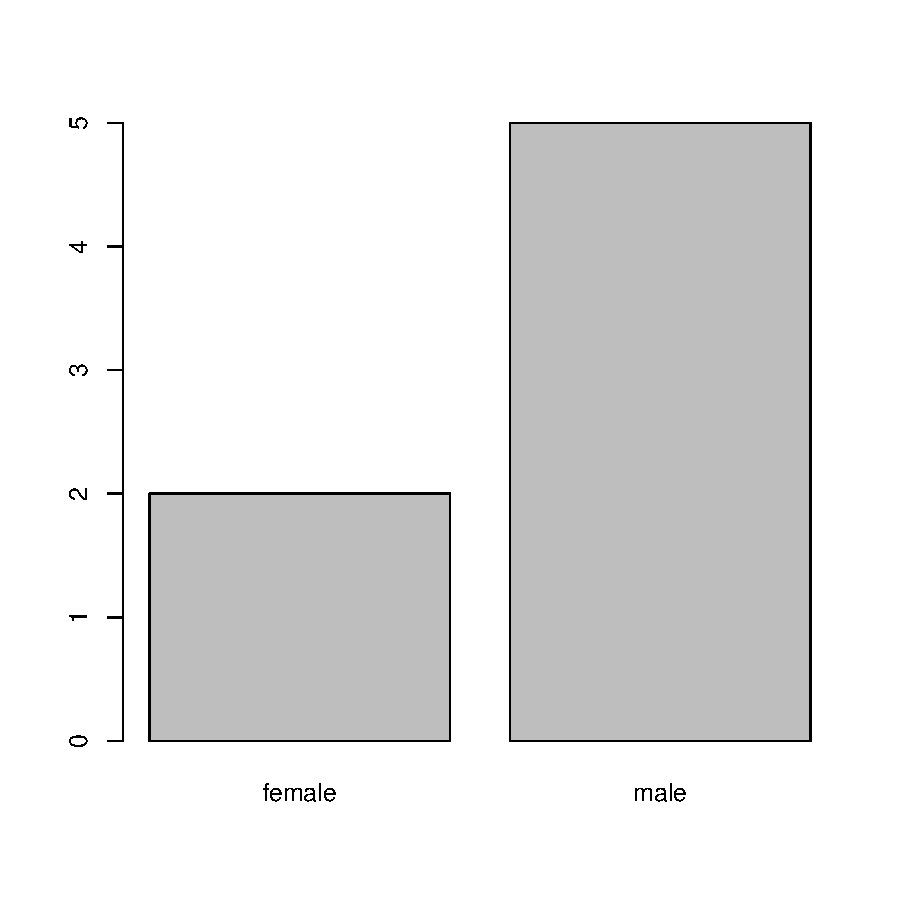
\includegraphics{r3-009}
Because we face a special type of object intended for categorical data - a factor with two levels (levels):

\begin{Schunk}
\begin{Sinput}
> is.factor(sex.f)
\end{Sinput}
\begin{Soutput}
[1] TRUE
\end{Soutput}
\begin{Sinput}
> is.character(sex.f)
\end{Sinput}
\begin{Soutput}
[1] FALSE
\end{Soutput}
\begin{Sinput}
> str(sex.f)
\end{Sinput}
\begin{Soutput}
 Factor w/ 2 levels "female","male": 2 1 2 2 1 2 2
NULL
\end{Soutput}
\end{Schunk}
Factor w / 2 levels "female", "male": 2 1 2 2 1 2 2

Very many of the functions in R (for example, the same plot()) prefer factors instead of text vectors. Additionally some are able to convert text into vector factors, and some are not, therefore, one has to be careful.
There are several other important properties of the factors that one needs to know in advance. First, a subset of factors is a factor with the same number of levels, even if they are not left in the subset:

\begin{Schunk}
\begin{Sinput}
> sex.f[5:6]
\end{Sinput}
\begin{Soutput}
[1] female male  
Levels: female male
\end{Soutput}
\begin{Sinput}
> sex.f[6:7]
\end{Sinput}
\begin{Soutput}
[1] male male
Levels: female male
\end{Soutput}
\end{Schunk}

One can get rid of an excess level only applying a special argument or by performing data conversion “to and back”:
\begin{Schunk}
\begin{Sinput}
> sex.f[6:7, drop = TRUE]
\end{Sinput}
\begin{Soutput}
[1] male male
Levels: male
\end{Soutput}
\begin{Sinput}
> factor(as.character(sex.f[6:7]))
\end{Sinput}
\begin{Soutput}
[1] male male
Levels: male
\end{Soutput}
\end{Schunk}
The factors as opposed to text vectors can be easily converted into the numerical values:
\begin{Schunk}
\begin{Sinput}
> as.numeric(sex.f)
\end{Sinput}
\begin{Soutput}
[1] 2 1 2 2 1 2 2
\end{Soutput}
\end{Schunk}

To understand why one have do it becomes clear if we consider here is an example: Suppose besides a height, we also have data on employees weight and we want to draw graph in which at the same time height, weight and gender will be displayed. Here is how to do that:

\begin{Schunk}
\begin{Sinput}
> w <- c(69, 68, 93, 87, 59, 82, 72)
\end{Sinput}
\begin{Soutput}
[1] 69 68 93 87 59 82 72
\end{Soutput}
\end{Schunk}
\begin{Schunk}
\begin{Sinput}
> plot(x, w, pch = as.numeric(sex.f), col = as.numeric(sex.f))
\end{Sinput}
\begin{Soutput}
NULL
\end{Soutput}
\begin{Sinput}
> legend("topleft", pch = 1:2, col = 1:2, legend = levels(sex.f))
\end{Sinput}
\begin{Soutput}
$rect
$rect$w
[1] 4.894687

$rect$h
[1] 4.269767

$rect$left
[1] 160.8

$rect$top
[1] 94.36


$text
$text$x
[1] 162.4875 162.4875

$text$y
[1] 92.93674 91.51349
\end{Soutput}
\end{Schunk}
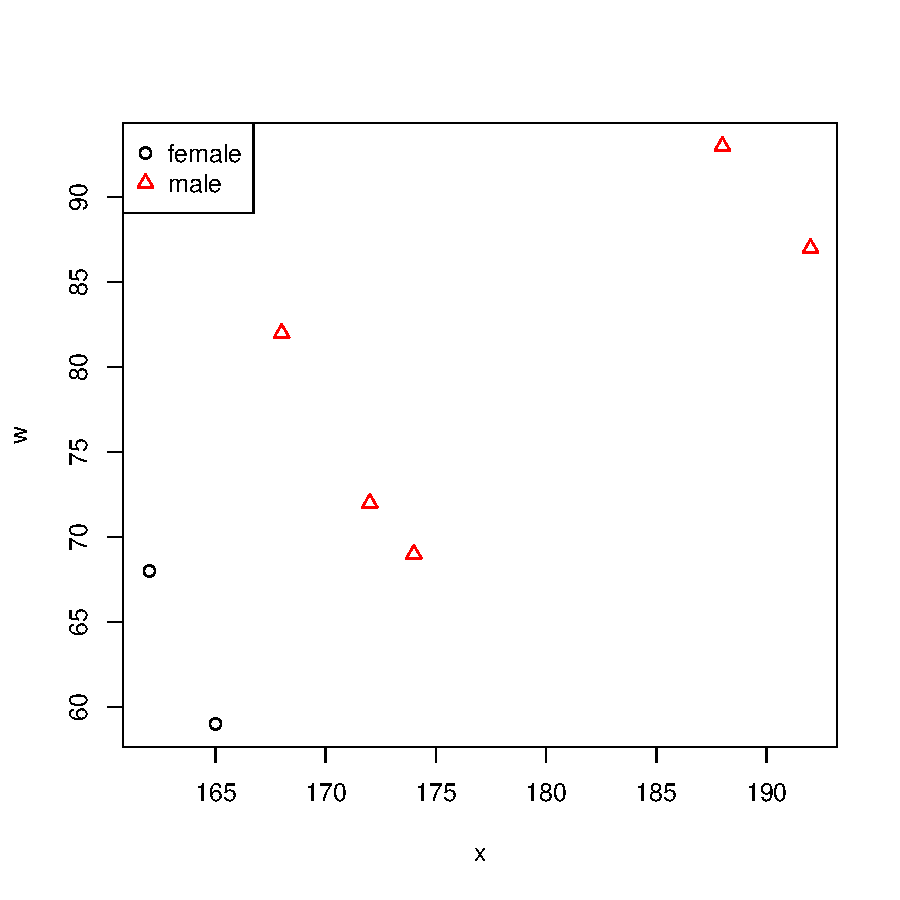
\includegraphics{r3-015}

Here, of course, some explanations are needed: pch and col are parameters which were assigned respectively to determine the icon types and their colors on the graph. Thus, depending on which sex this point belongs to, it will be displayed as a circle or a triangle, and black or red color respectively. It is required, of course, that all three vectors correspond each other. Yet it must be noted that the display of sex, using icon and color together is excessive, for a “normal” graph one method is enough.

Third, the factors can be sorted to convert them into some numerical data similarity. Let’s insert a fourth variable: T-shirts size for the same hypothetical eight employees:

\begin{Schunk}
\begin{Sinput}
> m <- c("L", "S", "XL", "XXL", "S", "M", "L")
\end{Sinput}
\begin{Soutput}
[1] "L"   "S"   "XL"  "XXL" "S"   "M"   "L"  
\end{Soutput}
\begin{Sinput}
> m.f <- factor(m)
\end{Sinput}
\begin{Soutput}
[1] L   S   XL  XXL S   M   L  
Levels: L M S XL XXL
\end{Soutput}
\begin{Sinput}
> m.f
\end{Sinput}
\begin{Soutput}
[1] L   S   XL  XXL S   M   L  
Levels: L M S XL XXL
\end{Soutput}
\end{Schunk}

As you can see, the levels are sorted in alphabetical order but we need to "S" (small) to come first. Furthermore, we must somehow inform R that we have not simple categorical data but orderable categorical data. One should do that as follows:
\begin{Schunk}
\begin{Sinput}
> m.o <- ordered(m.f, levels = c("S", "M", "L", "XL", "XXL"))
\end{Sinput}
\begin{Soutput}
[1] L   S   XL  XXL S   M   L  
Levels: S < M < L < XL < XXL
\end{Soutput}
\begin{Sinput}
> m.o
\end{Sinput}
\begin{Soutput}
[1] L   S   XL  XXL S   M   L  
Levels: S < M < L < XL < XXL
\end{Soutput}
\end{Schunk}

\section{Missing data}
\label{sec:missdata}

In addition to the vectors of numbers and text vectors, R supports also logical vectors, as well as special data types that can be very important for statistical calculations. First of all, it's skipped or missing data, which are denoted as NA. Such data are often arising in the real field and laboratory studies, surveys, polls, tests etc. It should be aware that the presence of missing data does not mean that the data are generally of poor quality. On the other hand, statistical programs must somehow work with that data also. Let us consider the following example: suppose that we have the result of a survey of the same seven employees. They were asked how many hours they averagely sleep but one of the respondents refused to answer, another said “I do not know” and the third one was out of the office at the moment of in the survey. Than was how missing data were aroused:
\begin{Schunk}
\begin{Sinput}
> h <- c(8, 10, NA, NA, 8, NA, 8)
\end{Sinput}
\begin{Soutput}
[1]  8 10 NA NA  8 NA  8
\end{Soutput}
\begin{Sinput}
> h
\end{Sinput}
\begin{Soutput}
[1]  8 10 NA NA  8 NA  8
\end{Soutput}
\end{Schunk}

This example shows that NA should be entered without quotation marks, and R is not in the least embarrassed that among the numbers some kind of text arrives. Note that the missing data are often as diverse as in our example. However, they are coded in the same way, and this must not be forgotten. Now, about how to work with the obtained vector h. If we just try to calculate the mean value (function mean()), we obtain:
\begin{Schunk}
\begin{Sinput}
> mean(h)
\end{Sinput}
\begin{Soutput}
[1] NA
\end{Soutput}
\end{Schunk}
And it is “ideologically correct” because the function may differently process NA, and by default, it simply indicates that something is wrong with the data. To calculate the average of “not missed” part of the vector one can use one of two ways:
\begin{Schunk}
\begin{Sinput}
> mean(h, na.rm = TRUE)
\end{Sinput}
\begin{Soutput}
[1] 8.5
\end{Soutput}
\begin{Sinput}
> mean(na.omit(h))
\end{Sinput}
\begin{Soutput}
[1] 8.5
\end{Soutput}
\end{Schunk}

Which way is better depends on the situation. One problem more often arrives: how to make a substitution of missing data, for example, replace all NA with the average for the sample. A common solution is like the following:

\begin{Schunk}
\begin{Sinput}
> h[is.na(h)] <- mean(h, na.rm = TRUE)
\end{Sinput}
\begin{Soutput}
[1] 8.5
\end{Soutput}
\begin{Sinput}
> h
\end{Sinput}
\begin{Soutput}
[1]  8.0 10.0  8.5  8.5  8.0  8.5  8.0
\end{Soutput}
\end{Schunk}
On the left side of the first expression indexing is on the run, it is selection of values in h to replace missing numbers (is.na ()). After the expression execution "old" values disappear forever.

\section{Matrixes}
\label{sec:matrix}

A matrix is extremely widespread form of data representation presented in a form of table. Concerning matrixes R one must generally know two important things: first, that they may be of different dimensions, and secondly, that there are really no matrixes R.
Let's start with the last. Matrix in R is simply a special type of vector which possesses some additional properties (“attributes”), allowing to interpret it as a set of rows and columns. Suppose we want to create a simple \(2\times2\). To start with let’s create it from a numerical vector:
\begin{Schunk}
\begin{Sinput}
> m <- 1:4
\end{Sinput}
\begin{Soutput}
[1] 1 2 3 4
\end{Soutput}
\begin{Sinput}
> m
\end{Sinput}
\begin{Soutput}
[1] 1 2 3 4
\end{Soutput}
\begin{Sinput}
> ma <- matrix(m, ncol = 2, byrow = TRUE)
\end{Sinput}
\begin{Soutput}
     [,1] [,2]
[1,]    1    2
[2,]    3    4
\end{Soutput}
\begin{Sinput}
> ma
\end{Sinput}
\begin{Soutput}
     [,1] [,2]
[1,]    1    2
[2,]    3    4
\end{Soutput}
\begin{Sinput}
> str(ma)
\end{Sinput}
\begin{Soutput}
 int [1:2, 1:2] 1 3 2 4
NULL
\end{Soutput}
\begin{Sinput}
> str(m)
\end{Sinput}
\begin{Soutput}
 int [1:4] 1 2 3 4
NULL
\end{Soutput}
\end{Schunk}

This example shows that the structure of the object m and ma are not too different. The only difference is in their screen display. Even more obvious unity between vectors and matrices can be traced if you create a matrix in a different way:
\begin{Schunk}
\begin{Sinput}
> mb <- m
\end{Sinput}
\begin{Soutput}
[1] 1 2 3 4
\end{Soutput}
\begin{Sinput}
> mb
\end{Sinput}
\begin{Soutput}
[1] 1 2 3 4
\end{Soutput}
\begin{Sinput}
> attr(mb, "dim") <- c(2, 2)
\end{Sinput}
\begin{Soutput}
[1] 2 2
\end{Soutput}
\begin{Sinput}
> mb
\end{Sinput}
\begin{Soutput}
     [,1] [,2]
[1,]    1    3
[2,]    2    4
\end{Soutput}
\end{Schunk}
It looks like a trick. However, everything is simple: we assign a vector mb an attribute dim (from the word dimension) and set the value of this attribute in c(2,2), there are two rows and two columns. A reader is expected to guess why mb matrix is different from ma one (the answer at end of the article). 
We showed only two ways to create matrices, but in reality there are much more. It is very popular, for example, to make the matrices of vector-columns or rows using commands cbind() and rbind (). If the result must be turned in 90 degrees, use the command t().
The most common are matrices with two dimensions but nobody prevents to make a multi-dimensional matrix:
 \(2\times2\times2\):
\begin{Schunk}
\begin{Sinput}
> m3 <- 1:8
\end{Sinput}
\begin{Soutput}
[1] 1 2 3 4 5 6 7 8
\end{Soutput}
\begin{Sinput}
> dim(m3) <- c(2, 2, 2)
\end{Sinput}
\begin{Soutput}
[1] 2 2 2
\end{Soutput}
\begin{Sinput}
> m3
\end{Sinput}
\begin{Soutput}
, , 1

     [,1] [,2]
[1,]    1    3
[2,]    2    4

, , 2

     [,1] [,2]
[1,]    5    7
[2,]    6    8
\end{Soutput}
\end{Schunk}
m3 is a three-dimensional matrix. Naturally one is not able to show it as a table, therefore R displays it on the screen as a series of tables. Similarly one can create also four-dimensional matrix (like built-in Titanic data from the previous article). Multi-dimensional matrices in R are called arrays.

\section{Lists}
\label{sec:lists}

Lists are another very important type of data representation. Their creation, especially at first, probably will not be necessary, but one needs to know their characters. It is needed mainly because very many functions in R return the very lists. At the very beginning of acquaintance let’s create a list just for a practice:

\begin{Schunk}
\begin{Sinput}
> l <- list("R", 1:3, TRUE, NA, list("r", 4))
\end{Sinput}
\begin{Soutput}
[[1]]
[1] "R"

[[2]]
[1] 1 2 3

[[3]]
[1] TRUE

[[4]]
[1] NA

[[5]]
[[5]][[1]]
[1] "r"

[[5]][[2]]
[1] 4
\end{Soutput}
\begin{Sinput}
> l
\end{Sinput}
\begin{Soutput}
[[1]]
[1] "R"

[[2]]
[1] 1 2 3

[[3]]
[1] TRUE

[[4]]
[1] NA

[[5]]
[[5]][[1]]
[1] "r"

[[5]][[2]]
[1] 4
\end{Soutput}
\end{Schunk}

We see that the list some kind of assortment. A vector and, accordingly, a matrix may consist only of elements of the same type, but a list can consist of anything. In particular, as one can see from the example, a list may include other lists. Now let's talk about indexing or selecting list items. Elements of the vector are selected by means of the square brackets function:

\begin{Schunk}
\begin{Sinput}
> l[3]
\end{Sinput}
\begin{Soutput}
[[1]]
[1] TRUE
\end{Soutput}
\end{Schunk}
The matrix elements can be chosen the same way, only several arguments are in use (for two-dimensional matrix it is the row number and the column number, in this order):
\begin{Schunk}
\begin{Sinput}
> ma[2, 1]
\end{Sinput}
\begin{Soutput}
[1] 3
\end{Soutput}
\end{Schunk}
But the list items are selected by three different methods. First, you can use square brackets:
\begin{Schunk}
\begin{Sinput}
> l[1]
\end{Sinput}
\begin{Soutput}
[[1]]
[1] "R"
\end{Soutput}
\begin{Sinput}
> str(l[1])
\end{Sinput}
\begin{Soutput}
List of 1
 $ : chr "R"
NULL
\end{Soutput}
\end{Schunk}
It is very important here that the resulting object will be also list. Secondly double square brackets can be used:
\begin{Schunk}
\begin{Sinput}
> l[[1]]
\end{Sinput}
\begin{Soutput}
[1] "R"
\end{Soutput}
\begin{Sinput}
> str(l[[1]])
\end{Sinput}
\begin{Soutput}
 chr "R"
NULL
\end{Soutput}
\end{Schunk}

In this case, the resulting object will be of the same type as it would be before to the unification to the list (and therefore the first object is a text vector and a fifth is a list). Third, you can use the list names. But t first you must assign them:
\begin{Schunk}
\begin{Sinput}
> names(l) <- c("first", "second", "third", "fourth", "fifth")
\end{Sinput}
\begin{Soutput}
[1] "first"  "second" "third"  "fourth" "fifth" 
\end{Soutput}
\begin{Sinput}
> str(l$first)
\end{Sinput}
\begin{Soutput}
 chr "R"
NULL
\end{Soutput}
\end{Schunk}

To select by a name the dollar sign is used, and the resulting object will be the same as using double square brackets. In fact, the names in R can have vector elements and matrix rows and columns:

\begin{Schunk}
\begin{Sinput}
> names(w) <- c("Nic", "John", "Piter", "Alex", "Cat", "Bob", "Gorge")
\end{Sinput}
\begin{Soutput}
[1] "Nic"   "John"  "Piter" "Alex"  "Cat"   "Bob"   "Gorge"
\end{Soutput}
\begin{Sinput}
> w
\end{Sinput}
\begin{Soutput}
  Nic  John Piter  Alex   Cat   Bob Gorge 
   69    68    93    87    59    82    72 
\end{Soutput}
\begin{Sinput}
> w["John"]
\end{Sinput}
\begin{Soutput}
John 
  68 
\end{Soutput}
\begin{Sinput}
> rownames(ma) <- c("a1", "a2")
\end{Sinput}
\begin{Soutput}
[1] "a1" "a2"
\end{Soutput}
\begin{Sinput}
> colnames(ma) <- c("b1", "b2")
\end{Sinput}
\begin{Soutput}
[1] "b1" "b2"
\end{Soutput}
\begin{Sinput}
> ma
\end{Sinput}
\begin{Soutput}
   b1 b2
a1  1  2
a2  3  4
\end{Soutput}
\end{Schunk}

\section{Data Tables}
\label{sec:tables}

Finally we came to the most important type of data - data tables (data frames). Those very data tables are the most similar to Excel spreadsheets and their analogues, and therefore are in the most often use. It is especially true for R beginners. Data tables are hybrid type of same length vectors representation, a one-dimensional list of vectors of the same length. Thus, each data table is a list of columns and within the same column, all data must be of one type. We illustrate this by an example concerning vectors created in this article before:

\begin{Schunk}
\begin{Sinput}
> d <- data.frame(weight = w, height = x, size = m.o, sex = sex.f)
\end{Sinput}
\begin{Soutput}
      weight height size    sex
Nic       69    174    L   male
John      68    162    S female
Piter     93    188   XL   male
Alex      87    192  XXL   male
Cat       59    165    S female
Bob       82    168    M   male
Gorge     72    172    L   male
\end{Soutput}
\begin{Sinput}
> d
\end{Sinput}
\begin{Soutput}
      weight height size    sex
Nic       69    174    L   male
John      68    162    S female
Piter     93    188   XL   male
Alex      87    192  XXL   male
Cat       59    165    S female
Bob       82    168    M   male
Gorge     72    172    L   male
\end{Soutput}
\begin{Sinput}
> str(d)
\end{Sinput}
\begin{Soutput}
'data.frame':	7 obs. of  4 variables:
 $ weight: num  69 68 93 87 59 82 72
 $ height: num  174 162 188 192 165 168 172
 $ size  : Ord.factor w/ 5 levels "S"<"M"<"L"<"XL"<..: 3 1 4 5 1 2 3
 $ sex   : Factor w/ 2 levels "female","male": 2 1 2 2 1 2 2
NULL
\end{Soutput}
\end{Schunk}



Because the data table is a list, list indexing methods are applicable to it. Furthermore, data tables can be indexed as a two-dimensional matrix. Here are some examples:

\begin{Schunk}
\begin{Sinput}
> d$weight
\end{Sinput}
\begin{Soutput}
[1] 69 68 93 87 59 82 72
\end{Soutput}
\begin{Sinput}
> d[[1]]
\end{Sinput}
\begin{Soutput}
[1] 69 68 93 87 59 82 72
\end{Soutput}
\begin{Sinput}
> d[, 1]
\end{Sinput}
\begin{Soutput}
[1] 69 68 93 87 59 82 72
\end{Soutput}
\begin{Sinput}
> d[, "weight"]
\end{Sinput}
\begin{Soutput}
[1] 69 68 93 87 59 82 72
\end{Soutput}
\end{Schunk}

It is often necessary to select a few specific columns. This can be done but in different ways (exclude the column weight):
\begin{Schunk}
\begin{Sinput}
> d[, 2:4]
\end{Sinput}
\begin{Soutput}
      height size    sex
Nic      174    L   male
John     162    S female
Piter    188   XL   male
Alex     192  XXL   male
Cat      165    S female
Bob      168    M   male
Gorge    172    L   male
\end{Soutput}
\begin{Sinput}
> d[, -1]
\end{Sinput}
\begin{Soutput}
      height size    sex
Nic      174    L   male
John     162    S female
Piter    188   XL   male
Alex     192  XXL   male
Cat      165    S female
Bob      168    M   male
Gorge    172    L   male
\end{Soutput}
\end{Schunk}

The second method (negative indexing) in some cases is practically unreplacable. Indexing is directly connected to one more R data type – logical vectors. For example, how can we select from our table the data related to women only? Here's one way:
\begin{Schunk}
\begin{Sinput}
> d$sex == "female"
\end{Sinput}
\begin{Soutput}
[1] FALSE  TRUE FALSE FALSE  TRUE FALSE FALSE
\end{Soutput}
\begin{Sinput}
> d[d$sex == "female", ]
\end{Sinput}
\begin{Soutput}
     weight height size    sex
John     68    162    S female
Cat      59    165    S female
\end{Soutput}
\end{Schunk}

Thus, after the selection “processing”, the data in the table contains only those rows that correspond to "TRUE, so the lines 2 and 5.
A more complex selection case is the data tables sorting. To sort a vector it is sufficient to apply the command sort(), but if necessary, for example, to sort our data is first on sex, and then on the height, we have to user a more difficult operation:

\begin{Schunk}
\begin{Sinput}
> d[order(d$sex, d$height), ]
\end{Sinput}
\begin{Soutput}
      weight height size    sex
John      68    162    S female
Cat       59    165    S female
Bob       82    168    M   male
Gorge     72    172    L   male
Nic       69    174    L   male
Piter     93    188   XL   male
Alex      87    192  XXL   male
\end{Soutput}
\end{Schunk}

From all ways data exchange from Excel with R through clipboard may be the most attractive. If to open in OpenOffice Calc a xls-file it is possible to copy any quantity of cells in the buffer, and then for  putting  them in R you may  use next command:\\
t<-read.table("clipboard");\\
Another way, is read from file\\
t<-read.table("<name_file.txt>",sep=';')\\




\section{Vectorized computation}
\label{sec:vectorcount}

Despite the fact that R is similar to many modern script programming languages, such as Perl and Python, it has many peculiar features. One of the interesting and very useful features of the R this so called vectorized computations. Their use is very simple. Suppose we want to transfer weight from pounds to grams:

\begin{Schunk}
\begin{Sinput}
> w * 1000
\end{Sinput}
\begin{Soutput}
  Nic  John Piter  Alex   Cat   Bob Gorge 
69000 68000 93000 87000 59000 82000 72000 
\end{Soutput}
\end{Schunk}

For such an operation it is often required to use looping constructs (loops) but here we use one operation only. Of course loops also will work in \R:
\begin{Schunk}
\begin{Sinput}
> for (i in seq_along(w)) {
+     w[i] <- w[i] * 1000
+ }
\end{Sinput}
\begin{Soutput}
NULL
\end{Soutput}
\begin{Sinput}
> w
\end{Sinput}
\begin{Soutput}
  Nic  John Piter  Alex   Cat   Bob Gorge 
69000 68000 93000 87000 59000 82000 72000 
\end{Soutput}
\end{Schunk}


But this is too cumbersome. Operation on vectors and matrices are also vectorised:
\begin{Schunk}
\begin{Sinput}
> ma + mb
\end{Sinput}
\begin{Soutput}
   b1 b2
a1  2  5
a2  5  8
\end{Soutput}
\begin{Sinput}
> 1:8 + 1:2
\end{Sinput}
\begin{Soutput}
[1]  2  4  4  6  6  8  8 10
\end{Soutput}
\end{Schunk}

\section{If}
\label{sec:If}
The if/else statement conditionally evaluates two statements. There is a condition which is evaluated and if the value is TRUE then the first statement is evaluated; otherwise the second statement will be evaluated. The if/else statement returns, as its value, the value of the statement that was selected. The formal syntax is

     if ( statement1 ) {
         command1
         command2
         
         }
     else
        {
        command3
        command4
        }      
        


If/else statements can be nested.

     if ( statement1 )
         statement2
     else if ( statement3 )
         statement4
     else if ( statement5 )
         statement6
     else
         statement8
One of the even numbered statements will be evaluated and the resulting value returned. If the optional else clause is omitted and all the odd numbered statement's evaluate to FALSE no statement will be evaluated and NULL is returned.

The odd numbered statements are evaluated, in order, until one evaluates to TRUE and then the associated even numbered statement is evaluated. In this example, statement6 will only be evaluated if statement1 is FALSE and statement3 is FALSE and statement5 is TRUE. There is no limit to the number of else if clauses that are permitted.

\section{For}
\label{sec:For}
The syntax of the for loop is

     for ( name in vector )
        
        statement1
        
        
where vector can be either a vector or a list. For each element in vector the variable name is set to the value of that element and statement1 is evaluated. A side effect is that the variable name still exists after the loop has concluded and it has the value of the last element of vector that the loop was evaluated for.

\section{While}
\label{sec:While}
The while statement is very similar to the repeat statement. The syntax of the while loop is

     while ( statement1 ) statement2
     
where statement1 is evaluated and if its value is TRUE then statement2 is evaluated. This process continues until statement1 evaluates to FALSE.


\section{Example}
\label{sec:Example}
Now I want to show you  the  one program for example.
This program take data from  central bank of Czech Republic  and create the matrix of correlation.

I will show it program in RStudio.
Now please  run Rstudio and  create program on  the   computers yourself.

\begin{Schunk}
\begin{Soutput}
NULL
\end{Soutput}
\begin{Soutput}
$timeout
[1] 60
\end{Soutput}
\begin{Soutput}
         Datum X1.AUD X1.BGN X1.BRL X1.CAD X1.CHF X1.CNY X1.DKK X1.EUR X1.GBP
1   03.01.2011 19.175 12.827 11.371 18.968 20.119  2.852  3.366 25.085 29.123
2   04.01.2011 18.714 12.724 11.224 18.665 19.644  2.807  3.339 24.885 28.976
3   05.01.2011 18.811 12.706 11.308 18.811 19.705  2.858  3.337 24.870 29.293
4   06.01.2011 18.805 12.634 11.205 18.987 19.491  2.848  3.316 24.710 29.245
5   07.01.2011 18.805 12.559 11.218 19.097 19.632  2.860  3.297 24.565 29.299
6   10.01.2011 18.910 12.601 11.295 19.181 19.782  2.878  3.309 24.650 29.632
7   11.01.2011 18.686 12.550 11.231 19.117 19.578  2.864  3.295 24.545 29.506
8   12.01.2011 18.616 12.468 11.188 19.073 19.318  2.847  3.273 24.385 29.322
9   13.01.2011 18.463 12.459 11.052 18.670 19.007  2.796  3.271 24.370 29.160
10  14.01.2011 18.013 12.467 10.831 18.326 18.879  2.771  3.273 24.385 28.951
11  17.01.2011 18.202 12.444 10.886 18.523 18.930  2.773  3.267 24.340 29.110
12  18.01.2011 18.114 12.423 10.862 18.430 18.967  2.760  3.261 24.295 29.076
13  19.01.2011 18.075 12.406 10.779 18.122 18.720  2.730  3.256 24.260 28.778
14  20.01.2011 17.971 12.480 10.839 18.132 18.963  2.751  3.276 24.410 28.935
15  21.01.2011 17.778 12.418 10.746 18.028 18.665  2.729  3.259 24.290 28.636
16  24.01.2011 17.693 12.382 10.675 17.941 18.644  2.711  3.250 24.220 28.437
17  25.01.2011 17.650 12.386 10.656 17.816 18.815  2.706  3.251 24.230 28.101
18  26.01.2011 17.648 12.382 10.617 17.767 18.749  2.689  3.250 24.220 28.052
19  27.01.2011 17.507 12.395 10.578 17.754 18.730  2.685  3.252 24.240 28.197
20  28.01.2011 17.637 12.397 10.561 17.766 18.734  2.687  3.253 24.245 28.164
21  31.01.2011 17.604 12.386 10.569 17.711 18.793  2.681  3.250 24.230 28.138
22  01.02.2011 17.669 12.325 10.527 17.577 18.609  2.658  3.233 24.105 28.242
23  02.02.2011 17.649 12.335 10.506 17.689 18.660  2.666  3.236 24.125 28.316
24  03.02.2011 17.740 12.317 10.512 17.719 18.555  2.674  3.232 24.095 28.389
25  04.02.2011 17.910 12.276 10.576 17.854 18.531  2.687  3.221 24.010 28.342
26  07.02.2011 18.019 12.308 10.606 17.986 18.582  2.706  3.229 24.070 28.640
27  08.02.2011 17.856 12.281 10.511 17.785 18.434  2.689  3.222 24.020 28.304
28  09.02.2011 17.920 12.377 10.635 17.843 18.407  2.691  3.247 24.210 28.483
29  10.02.2011 17.885 12.396 10.681 17.864 18.497  2.706  3.252 24.245 28.593
30  11.02.2011 17.916 12.401 10.742 18.010 18.425  2.720  3.253 24.255 28.678
31  14.02.2011 18.048 12.392 10.814 18.252 18.550  2.734  3.250 24.235 28.855
32  15.02.2011 17.977 12.419 10.791 18.241 18.503  2.729  3.257 24.290 29.006
33  16.02.2011 18.002 12.437 10.795 18.260 18.598  2.733  3.262 24.325 28.889
34  17.02.2011 18.020 12.440 10.759 18.252 18.758  2.724  3.263 24.325 28.932
35  18.02.2011 18.072 12.458 10.724 18.180 18.780  2.720  3.270 24.375 29.018
36  21.02.2011 18.091 12.506 10.754 18.192 18.869  2.725  3.280 24.455 29.023
37  22.02.2011 17.962 12.524 10.743 18.155 19.054  2.724  3.286 24.495 28.953
38  23.02.2011 17.907 12.532 10.703 17.998 19.076  2.716  3.288 24.515 28.991
39  24.02.2011 17.927 12.539 10.674 18.103 19.245  2.710  3.291 24.530 28.818
40  25.02.2011 18.037 12.520 10.723 18.157 19.131  2.708  3.285 24.490 28.631
41  28.02.2011 17.901 12.449 10.621 17.987 18.956  2.678  3.266 24.350 28.552
42  01.03.2011 17.940 12.450 10.612 18.171 18.951  2.680  3.266 24.350 28.661
43  02.03.2011 17.828 12.419 10.591 18.058 18.953  2.676  3.258 24.290 28.651
44  03.03.2011 17.788 12.377 10.555 17.971 18.848  2.660  3.247 24.210 28.439
45  04.03.2011 17.623 12.425 10.569 17.908 18.703  2.652  3.260 24.310 28.331
46  07.03.2011 17.552 12.384 10.435 17.788 18.688  2.635  3.249 24.225 28.132
47  08.03.2011 17.583 12.388 10.539 17.895 18.711  2.654  3.249 24.230 28.158
48  09.03.2011 17.647 12.415 10.600 18.016 18.788  2.658  3.256 24.280 28.270
49  10.03.2011 17.678 12.458 10.637 18.166 18.868  2.682  3.267 24.365 28.445
50  11.03.2011 17.673 12.442 10.625 18.040 18.949  2.687  3.263 24.335 28.258
51  14.03.2011 17.579 12.445 10.494 17.902 18.810  2.658  3.263 24.335 28.110
52  15.03.2011 17.298 12.472 10.493 17.707 19.118  2.673  3.271 24.395 28.129
53  16.03.2011 17.325 12.462 10.519 17.738 19.110  2.659  3.268 24.375 28.110
54  17.03.2011 17.167 12.475 10.444 17.667 19.319  2.650  3.271 24.400 28.121
55  18.03.2011 17.124 12.469 10.339 17.549 19.115  2.627  3.270 24.385 27.906
56  21.03.2011 17.340 12.512 10.371 17.653 19.058  2.626  3.281 24.470 28.071
57  22.03.2011 17.410 12.497 10.338 17.570 19.034  2.625  3.278 24.445 28.169
58  23.03.2011 17.431 12.485 10.392 17.579 19.157  2.634  3.275 24.420 28.070
59  24.03.2011 17.680 12.551 10.486 17.767 19.153  2.650  3.292 24.550 28.086
60  25.03.2011 17.762 12.539 10.476 17.799 18.990  2.650  3.288 24.525 27.940
61  28.03.2011 17.944 12.550 10.528 17.871 19.023  2.666  3.291 24.545 27.950
62  29.03.2011 17.822 12.534 10.488 17.848 18.921  2.657  3.287 24.515 27.813
63  30.03.2011 17.942 12.540 10.606 17.937 18.873  2.655  3.289 24.525 27.901
64  31.03.2011 17.864 12.547 10.645 17.800 18.871  2.640  3.291 24.540 27.773
65  01.04.2011 17.961 12.533 10.651 17.916 18.767  2.648  3.287 24.510 27.808
66  04.04.2011 17.827 12.507 10.689 17.829 18.635  2.627  3.281 24.465 27.762
67  05.04.2011 17.798 12.495 10.708 17.871 18.666  2.638  3.277 24.440 27.999
68  06.04.2011 17.737 12.484 10.649 17.807 18.643  2.610  3.275 24.420 27.827
69  07.04.2011 17.938 12.486 10.696 17.840 18.625  2.615  3.277 24.435 27.893
70  08.04.2011 17.845 12.489 10.789 17.772 18.555  2.595  3.275 24.425 27.725
71  11.04.2011 17.837 12.494 10.759 17.687 18.615  2.589  3.277 24.435 27.662
72  12.04.2011 17.733 12.498 10.705 17.635 18.783  2.583  3.278 24.445 27.515
73  13.04.2011 17.661 12.475 10.626 17.505 18.778  2.577  3.272 24.400 27.416
74  14.04.2011 17.686 12.404 10.597 17.443 18.833  2.579  3.253 24.260 27.491
75  15.04.2011 17.631 12.377 10.620 17.374 18.767  2.565  3.246 24.210 27.389
76  18.04.2011 17.816 12.366 10.687 17.564 18.870  2.595  3.243 24.190 27.566
77  19.04.2011 17.711 12.335 10.652 17.619 18.784  2.583  3.235 24.125 27.475
78  20.04.2011 17.761 12.359 10.649 17.514 18.674  2.552  3.242 24.175 27.266
79  21.04.2011 17.825 12.365 10.582 17.489 18.814  2.554  3.243 24.185 27.444
80  22.04.2011 17.809 12.336 10.606 17.396 18.731  2.549  3.236 24.130 27.375
81  26.04.2011 17.737 12.325 10.530 17.306 18.779  2.527  3.233 24.105 27.173
82  27.04.2011 17.801 12.336 10.566 17.279 18.721  2.527  3.237 24.135 27.224
83  28.04.2011 17.751 12.333 10.369 17.152 18.622  2.508  3.235 24.125 27.137
84  29.04.2011 17.851 12.379 10.331 17.164 18.815  2.510  3.247 24.210 27.149
85  02.05.2011 17.838 12.362 10.357 17.160 18.808  2.511  3.243 24.180 27.187
86  03.05.2011 17.772 12.361 10.292 17.155 18.910  2.518  3.242 24.175 26.951
87  04.05.2011 17.640 12.378 10.268 17.077 18.889  2.505  3.247 24.210 26.900
88  05.05.2011 17.417 12.369 10.130 16.905 19.006  2.514  3.244 24.190 26.914
89  06.05.2011 17.744 12.319 10.276 17.243 19.023  2.559  3.231 24.095 27.262
90  09.05.2011 18.060 12.361 10.434 17.415 19.161  2.586  3.243 24.180 27.500
91  10.05.2011 18.223 12.388 10.479 17.587 19.228  2.599  3.250 24.230 27.602
92  11.05.2011 18.303 12.404 10.506 17.703 19.158  2.602  3.254 24.260 27.865
93  12.05.2011 18.213 12.414 10.543 17.753 19.289  2.639  3.256 24.275 27.896
94  13.05.2011 18.243 12.468 10.568 17.732 19.256  2.629  3.271 24.390 27.779
95  16.05.2011 18.202 12.461 10.580 17.687 19.435  2.649  3.269 24.375 27.939
96  17.05.2011 18.264 12.505 10.570 17.699 19.485  2.653  3.280 24.460 28.022
97  18.05.2011 18.232 12.527 10.646 17.675 19.532  2.648  3.286 24.500 27.821
98  19.05.2011 18.275 12.509 10.673 17.728 19.392  2.637  3.281 24.465 27.762
99  20.05.2011 18.319 12.517 10.625 17.735 19.622  2.649  3.283 24.480 27.913
100 23.05.2011 18.400 12.546 10.701 17.873 19.817  2.690  3.291 24.535 28.209
101 24.05.2011 18.432 12.565 10.726 17.831 19.807  2.684  3.296 24.575 28.157
102 25.05.2011 18.340 12.565 10.717 17.845 19.938  2.690  3.296 24.575 28.336
103 26.05.2011 18.412 12.596 10.709 17.781 19.960  2.679  3.304 24.635 28.368
104 27.05.2011 18.423 12.568 10.711 17.658 20.120  2.655  3.297 24.585 28.362
105 30.05.2011 18.356 12.532 10.774 17.597 20.175  2.649  3.287 24.510 28.266
106 31.05.2011 18.169 12.544 10.788 17.543 19.994  2.633  3.291 24.540 28.138
107 01.06.2011 18.257 12.526 10.783 17.557 20.136  2.625  3.286 24.500 27.935
108 02.06.2011 18.087 12.541 10.696 17.354 20.158  2.617  3.290 24.530 27.784
109 03.06.2011 17.984 12.496 10.702 17.243 20.042  2.604  3.279 24.445 27.541
110 06.06.2011 17.901 12.446 10.544 16.999 19.895  2.574  3.265 24.340 27.342
111 07.06.2011 17.681 12.381 10.487 16.936 19.783  2.550  3.247 24.215 27.134
112 08.06.2011 17.576 12.376 10.447 16.897 19.804  2.559  3.247 24.210 27.116
113 09.06.2011 17.496 12.339 10.459 16.878 19.714  2.550  3.236 24.135 27.133
114 10.06.2011 17.691 12.340 10.513 17.155 19.796  2.571  3.236 24.135 27.175
115 13.06.2011 17.763 12.341 10.554 17.197 20.069  2.593  3.236 24.135 27.404
116 14.06.2011 17.768 12.330 10.546 17.135 19.904  2.576  3.233 24.115 27.373
117 15.06.2011 18.089 12.382 10.661 17.470 19.905  2.615  3.246 24.215 27.530
118 16.06.2011 18.095 12.416 10.703 17.434 20.311  2.663  3.256 24.285 27.744
119 17.06.2011 17.956 12.339 10.587 17.278 19.938  2.614  3.235 24.130 27.338
120 20.06.2011 17.833 12.333 10.541 17.227 20.039  2.619  3.234 24.125 27.432
121 21.06.2011 17.844 12.378 10.596 17.265 19.965  2.605  3.246 24.210 27.303
122 22.06.2011 17.876 12.415 10.643 17.340 20.058  2.611  3.257 24.290 27.192
123 23.06.2011 18.007 12.450 10.776 17.583 20.349  2.649  3.265 24.350 27.374
124 24.06.2011 18.092 12.464 10.744 17.463 20.480  2.650  3.268 24.375 27.431
125 27.06.2011 17.958 12.494 10.751 17.384 20.625  2.654  3.277 24.440 27.468
126 28.06.2011 17.901 12.474 10.744 17.338 20.530  2.644  3.271 24.400 27.284
127 29.06.2011 17.918 12.447 10.744 17.342 20.223  2.611  3.264 24.345 27.056
128 30.06.2011 18.053 12.448 10.788 17.447 20.167  2.606  3.264 24.345 26.971
129 01.07.2011 17.982 12.431 10.744 17.412 19.821  2.596  3.260 24.315 26.865
130 04.07.2011 17.948 12.408 10.747 17.436 19.695  2.590  3.254 24.270 26.919
131 07.07.2011 18.295 12.414 10.886 17.707 20.112  2.636  3.255 24.280 27.218
132 08.07.2011 18.304 12.382 10.926 17.748 20.014  2.630  3.248 24.225 27.114
133 11.07.2011 18.364 12.358 10.886 17.746 20.635  2.660  3.241 24.175 27.453
134 12.07.2011 18.390 12.399 10.961 17.851 20.805  2.680  3.252 24.250 27.469
135 13.07.2011 18.496 12.473 11.010 18.037 20.860  2.681  3.271 24.395 27.645
136 14.07.2011 18.512 12.496 10.947 17.971 21.115  2.664  3.277 24.440 27.743
137 15.07.2011 18.463 12.521 10.998 18.072 21.155  2.679  3.284 24.490 27.906
138 18.07.2011 18.425 12.471 10.989 18.104 21.236  2.684  3.271 24.390 27.931
139 19.07.2011 18.448 12.521 11.009 18.093 21.102  2.676  3.284 24.490 27.866
140 20.07.2011 18.530 12.524 11.039 18.208 21.027  2.671  3.286 24.495 27.816
141 21.07.2011 18.409 12.471 10.995 18.129 20.861  2.657  3.275 24.405 27.753
142 22.07.2011 18.442 12.480 10.925 17.874 20.706  2.631  3.275 24.410 27.655
143 25.07.2011 18.409 12.469 10.938 17.933 21.090  2.631  3.272 24.390 27.640
144 26.07.2011 18.453 12.454 10.986 17.878 20.944  2.615  3.268 24.360 27.608
145 27.07.2011 18.564 12.417 10.816 17.828 20.972  2.610  3.259 24.290 27.506
146 28.07.2011 18.724 12.381 10.857 17.907 21.161  2.636  3.251 24.215 27.708
147 29.07.2011 18.534 12.368 10.794 17.844 21.189  2.636  3.247 24.190 27.649
148 01.08.2011 18.521 12.353 10.839 17.616 21.429  2.605  3.243 24.160 27.463
149 02.08.2011 18.528 12.385 10.865 17.789 21.932  2.656  3.253 24.230 27.792
150 03.08.2011 18.247 12.409 10.872 17.685 22.005  2.638  3.261 24.290 27.820
151 04.08.2011 18.050 12.430 10.874 17.578 22.071  2.654  3.264 24.310 27.896
152 05.08.2011 17.915 12.401 10.800 17.450 22.365  2.661  3.256 24.255 27.911
153 08.08.2011 17.620 12.370 10.655 17.247 22.300  2.644  3.248 24.195 27.841
154 09.08.2011 17.309 12.383 10.479 17.119 22.872  2.640  3.251 24.220 27.738
155 10.08.2011 17.337 12.315 10.476 17.042 23.038  2.612  3.233 24.085 27.235
156 11.08.2011 17.435 12.363 10.481 17.161 23.039  2.674  3.245 24.180 27.617
157 12.08.2011 17.547 12.365 10.506 17.199 22.013  2.656  3.247 24.185 27.594
158 15.08.2011 17.685 12.434 10.608 17.232 21.459  2.659  3.265 24.320 27.731
159 16.08.2011 17.683 12.468 10.600 17.216 21.781  2.661  3.274 24.385 27.757
160 17.08.2011 17.847 12.490 10.696 17.243 21.420  2.642  3.279 24.430 27.839
161 18.08.2011 17.758 12.485 10.644 17.225 21.402  2.661  3.278 24.420 28.050
162 19.08.2011 17.755 12.515 10.670 17.239 21.575  2.662  3.286 24.475 28.136
163 22.08.2011 17.769 12.521 10.655 17.254 21.596  2.654  3.288 24.490 28.035
164 23.08.2011 17.737 12.485 10.573 17.123 21.399  2.639  3.278 24.420 27.878
165 24.08.2011 17.788 12.524 10.595 17.167 21.485  2.656  3.288 24.495 27.922
166 25.08.2011 17.627 12.390 10.419 17.045 21.132  2.629  3.253 24.235 27.509
167 26.08.2011 17.603 12.356 10.422 16.970 21.087  2.627  3.243 24.165 27.287
168 29.08.2011 17.671 12.329 10.430 17.040 20.404  2.609  3.237 24.120 27.263
169 30.08.2011 17.798 12.321 10.475 17.074 20.337  2.620  3.234 24.095 27.254
170 31.08.2011 17.813 12.332 10.420 17.049 20.661  2.616  3.236 24.110 27.230
171 01.09.2011 18.093 12.348 10.567 17.307 21.157  2.650  3.242 24.150 27.406
172 02.09.2011 18.237 12.433 10.499 17.434 21.838  2.672  3.263 24.310 27.655
173 05.09.2011 18.293 12.504 10.488 17.511 22.010  2.712  3.284 24.460 27.948
174 06.09.2011 18.307 12.502 10.534 17.477 20.309  2.714  3.282 24.450 27.878
175 07.09.2011 18.484 12.501 10.528 17.619 20.282  2.724  3.283 24.450 27.843
176 08.09.2011 18.481 12.482 10.524 17.656 20.116  2.724  3.278 24.415 27.843
177 09.09.2011 18.612 12.489 10.599 17.806 20.079  2.768  3.281 24.430 28.215
178 12.09.2011 18.537 12.539 10.642 17.948 20.341  2.812  3.293 24.520 28.511
179 13.09.2011 18.576 12.548 10.507 18.122 20.392  2.812  3.296 24.545 28.443
180 14.09.2011 18.320 12.546 10.435 18.072 20.395  2.797  3.296 24.545 28.225
181 15.09.2011 18.279 12.543 10.384 17.987 20.336  2.781  3.293 24.525 28.098
182 16.09.2011 18.390 12.509 10.310 18.047 20.287  2.786  3.285 24.465 28.067
183 19.09.2011 18.488 12.597 10.304 18.353 20.425  2.826  3.308 24.635 28.380
184 20.09.2011 18.493 12.608 10.112 18.158 20.441  2.817  3.311 24.655 28.269
185 21.09.2011 18.662 12.750 10.095 18.341 20.423  2.865  3.347 24.930 28.558
186 22.09.2011 18.166 12.721  9.806 17.899 20.273  2.895  3.341 24.875 28.482
187 23.09.2011 17.971 12.714  9.678 17.950 20.394  2.898  3.342 24.870 28.510
188 26.09.2011 17.901 12.618 10.034 17.777 20.224  2.859  3.315 24.675 28.379
189 27.09.2011 17.879 12.517 10.002 17.684 20.024  2.818  3.290 24.480 28.148
190 29.09.2011 17.721 12.556  9.836 17.480 20.125  2.820  3.300 24.560 28.212
191 30.09.2011 17.844 12.656  9.877 17.548 20.342  2.874  3.326 24.755 28.558
192 03.10.2011 17.975 12.718  9.865 17.811 20.490  2.928  3.343 24.875 28.939
193 04.10.2011 17.819 12.735  9.949 17.891 20.469  2.963  3.347 24.910 29.059
194 05.10.2011 17.826 12.680 10.039 17.693 20.226  2.917  3.334 24.815 28.735
195 06.10.2011 18.104 12.704 10.209 17.894 20.166  2.938  3.338 24.845 28.659
196 07.10.2011 18.050 12.666 10.363 17.805 20.043  2.893  3.329 24.780 28.652
197 10.10.2011 18.113 12.666 10.452 17.717 20.100  2.872  3.328 24.775 28.512
198 11.10.2011 18.115 12.672 10.278 17.715 20.015  2.857  3.330 24.785 28.481
199 12.10.2011 18.220 12.677 10.149 17.714 20.040  2.833  3.331 24.795 28.327
200 13.10.2011 18.281 12.652 10.217 17.639 20.060  2.825  3.324 24.745 28.252
201 14.10.2011 18.372 12.648 10.290 17.659 19.972  2.809  3.323 24.740 28.279
202 17.10.2011 18.476 12.662 10.294 17.749 20.026  2.822  3.326 24.765 28.336
203 18.10.2011 18.467 12.735 10.256 17.769 20.174  2.855  3.346 24.910 28.623
204 19.10.2011 18.556 12.712 10.245 17.788 20.012  2.820  3.340 24.870 28.425
205 20.10.2011 18.517 12.731 10.210 17.767 20.146  2.826  3.344 24.900 28.466
206 21.10.2011 18.652 12.779 10.142 17.911 20.306  2.838  3.357 24.995 28.812
207 24.10.2011 18.757 12.775 10.138 17.926 20.344  2.829  3.356 24.985 28.746
208 25.10.2011 18.747 12.734 10.280 17.885 20.327  2.813  3.345 24.905 28.630
209 26.10.2011 18.572 12.746 10.192 17.666 20.441  2.818  3.349 24.930 28.591
210 27.10.2011 18.831 12.697 10.213 17.788 20.331  2.782  3.336 24.830 28.338
211 31.10.2011 18.757 12.680 10.495 17.806 20.344  2.788  3.332 24.800 28.404
212 01.11.2011 18.914 12.801 10.468 18.070 20.558  2.892  3.364 25.035 29.279
213 02.11.2011 18.909 12.859 10.480 17.996 20.677  2.866  3.380 25.150 29.176
214 03.11.2011 18.853 12.740 10.529 17.965 20.497  2.848  3.348 24.915 28.998
215 04.11.2011 18.822 12.781 10.438 17.801 20.455  2.862  3.358 24.995 29.022
216 07.11.2011 18.791 12.770 10.397 17.874 20.261  2.865  3.358 24.995 29.179
217 08.11.2011 18.873 12.872 10.480 18.014 20.331  2.877  3.382 25.175 29.339
218 09.11.2011 19.083 13.007 10.687 18.290 20.646  2.943  3.417 25.440 29.788
219 10.11.2011 19.041 13.036 10.639 18.357 20.705  2.952  3.427 25.500 29.879
220 11.11.2011 19.137 13.142 10.726 18.483 20.799  2.969  3.454 25.705 29.997
221 14.11.2011 19.284 13.161 10.689 18.535 20.814  2.966  3.458 25.740 30.047
222 15.11.2011 19.305 13.177 10.782 18.593 20.779  3.001  3.462 25.770 30.198
223 16.11.2011 19.208 13.084 10.681 18.502 20.661  2.991  3.438 25.590 29.945
    X1.HKD X1.HRK X100.HUF X1000.IDR X1.ILS X100.INR X100.JPY X100.KRW X1.LTL
1    2.419  3.397    9.011     2.090  5.307   42.107   23.075    1.672  7.265
2    2.387  3.368    9.024     2.063  5.260   41.174   22.584    1.657  7.207
3    2.422  3.368    8.976     2.095  5.312   41.462   22.784    1.670  7.203
4    2.428  3.350    8.952     2.098  5.299   41.679   22.681    1.686  7.156
5    2.438  3.318    8.863     2.099  5.291   41.667   22.680    1.683  7.114
6    2.456  3.331    8.791     2.110  5.333   41.959   23.000    1.689  7.139
7    2.437  3.315    8.790     2.096  5.346   41.973   22.814    1.685  7.109
8    2.418  3.295    8.852     2.082  5.304   41.690   22.537    1.687  7.062
9    2.375  3.294    8.875     2.040  5.179   40.954   22.254    1.662  7.058
10   2.348  3.296    8.816     2.017  5.135   40.177   22.015    1.632  7.062
11   2.351  3.292    8.861     2.018  5.152   40.135   22.144    1.640  7.049
12   2.336  3.287    8.913     2.007  5.142   39.956   22.031    1.633  7.036
13   2.310  3.283    8.906     1.985  5.083   39.562   21.888    1.617  7.026
14   2.328  3.302    8.878     2.000  5.004   39.709   22.001    1.613  7.069
15   2.307  3.285    8.858     1.983  4.945   39.386   21.715    1.604  7.035
16   2.288  3.275    8.837     1.969  4.926   39.092   21.532    1.590  7.014
17   2.285  3.271    8.807     1.971  4.924   38.867   21.609    1.587  7.017
18   2.273  3.268    8.831     1.959  4.906   38.929   21.529    1.584  7.014
19   2.269  3.271    8.888     1.958  4.843   38.748   21.276    1.589  7.020
20   2.270  3.268    8.923     1.959  4.815   38.636   21.496    1.587  7.022
21   2.269  3.266    8.848     1.956  4.764   38.588   21.543    1.580  7.017
22   2.249  3.250    8.875     1.939  4.739   38.295   21.491    1.573  6.981
23   2.245  3.251    8.948     1.938  4.749   38.368   21.457    1.569  6.987
24   2.252  3.247    8.931     1.943  4.750   38.443   21.419    1.574  6.978
25   2.262  3.238    8.881     1.959  4.735   38.616   21.549    1.581  6.954
26   2.281  3.247    8.944     1.983  4.817   39.037   21.581    1.607  6.971
27   2.264  3.240    8.921     1.974  4.788   38.900   21.428    1.595  6.957
28   2.278  3.265    8.915     1.987  4.842   39.044   21.488    1.598  7.012
29   2.288  3.271    8.872     1.996  4.823   38.948   21.508    1.590  7.022
30   2.301  3.273    8.930     2.007  4.862   39.269   21.461    1.589  7.025
31   2.314  3.271    8.897     2.023  4.911   39.635   21.612    1.602  7.019
32   2.307  3.279    8.960     2.017  4.930   39.537   21.456    1.604  7.035
33   2.311  3.284    8.983     2.024  4.986   39.557   21.500    1.608  7.045
34   2.303  3.283    9.034     2.019  4.955   39.521   21.462    1.607  7.045
35   2.296  3.290    9.026     2.018  4.928   39.581   21.439    1.609  7.059
36   2.299  3.301    9.024     2.020  4.969   39.784   21.510    1.597  7.082
37   2.300  3.306    8.981     2.019  4.931   39.589   21.554    1.590  7.094
38   2.291  3.308    8.995     2.017  4.916   39.565   21.565    1.590  7.100
39   2.285  3.304    8.972     2.008  4.869   39.165   21.765    1.568  7.104
40   2.283  3.299    8.974     2.012  4.883   39.257   21.766    1.580  7.093
41   2.259  3.278    8.994     1.995  4.853   38.879   21.493    1.562  7.052
42   2.261  3.281    8.932     1.998  4.853   39.181   21.469    1.570  7.052
43   2.258  3.272    8.954     1.996  4.838   39.242   21.429    1.562  7.035
44   2.244  3.265    8.938     1.985  4.842   38.806   21.342    1.562  7.011
45   2.236  3.282    8.936     1.981  4.813   38.718   21.024    1.562  7.040
46   2.217  3.271    8.919     1.965  4.798   38.328   21.038    1.547  7.016
47   2.238  3.275    8.888     1.984  4.868   38.711   21.133    1.557  7.017
48   2.238  3.280    8.904     1.984  4.889   38.729   21.084    1.565  7.032
49   2.263  3.296    8.925     2.008  4.949   39.034   21.223    1.570  7.056
50   2.268  3.292    8.920     2.013  4.937   39.050   21.489    1.568  7.048
51   2.239  3.293    8.911     1.992  4.913   38.762   21.324    1.550  7.048
52   2.253  3.304    8.902     2.002  4.905   38.743   21.728    1.547  7.065
53   2.241  3.305    8.918     1.991  4.920   38.773   21.681    1.542  7.059
54   2.233  3.308    8.915     1.985  4.894   38.622   22.109    1.538  7.067
55   2.212  3.304    8.922     1.968  4.871   38.328   21.266    1.531  7.062
56   2.210  3.316    9.025     1.976  4.880   38.307   21.267    1.536  7.087
57   2.207  3.314    9.039     1.972  4.878   38.238   21.226    1.536  7.080
58   2.216  3.308    9.058     1.981  4.877   38.515   21.343    1.536  7.072
59   2.229  3.324    9.198     1.994  4.870   38.863   21.467    1.553  7.110
60   2.229  3.320    9.210     1.994  4.892   38.891   21.404    1.562  7.103
61   2.243  3.322    9.182     2.007  4.938   39.012   21.421    1.570  7.109
62   2.236  3.319    9.161     1.998  4.950   38.946   21.213    1.566  7.100
63   2.236  3.324    9.182     1.996  4.959   38.896   20.957    1.581  7.103
64   2.220  3.327    9.236     1.984  4.964   38.736   20.867    1.579  7.107
65   2.228  3.323    9.207     1.993  4.987   38.980   20.674    1.588  7.098
66   2.209  3.319    9.222     1.983  4.959   38.721   20.459    1.578  7.085
67   2.218  3.316    9.242     1.991  4.975   38.828   20.463    1.584  7.078
68   2.196  3.313    9.275     1.973  4.932   38.579   20.046    1.573  7.072
69   2.201  3.315    9.249     1.971  4.951   38.729   20.070    1.571  7.077
70   2.183  3.316    9.249     1.960  4.937   38.482   19.886    1.567  7.074
71   2.179  3.317    9.210     1.956  4.917   38.138   19.989    1.557  7.077
72   2.173  3.318    9.179     1.951  4.902   38.249   20.059    1.547  7.080
73   2.165  3.312    9.163     1.945  4.940   37.825   20.020    1.550  7.067
74   2.166  3.292    9.074     1.944  4.915   38.043   20.236    1.546  7.026
75   2.155  3.287    9.062     1.934  4.900   37.793   20.111    1.538  7.012
76   2.179  3.286    9.048     1.954  4.930   38.115   20.454    1.552  7.006
77   2.169  3.279    9.033     1.944  4.908   37.946   20.409    1.549  6.987
78   2.142  3.286    9.168     1.925  4.881   37.561   20.126    1.542  7.002
79   2.134  3.287    9.168     1.922  4.871   37.358   20.232    1.532  7.004
80   2.134  3.279    9.112     1.922  4.873   37.525   20.248    1.534  6.988
81   2.122  3.276    9.117     1.906  4.830   37.037   20.179    1.521  6.981
82   2.117  3.282    9.115     1.908  4.811   37.053   19.993    1.524  6.990
83   2.098  3.278    9.128     1.900  4.777   36.682   19.946    1.518  6.987
84   2.097  3.287    9.153     1.902  4.809   36.846   20.060    1.524  7.012
85   2.098  3.283    9.166     1.907  4.832   36.757   20.007    1.529  7.003
86   2.105  3.276    9.105     1.915  4.825   36.744   20.253    1.526  7.001
87   2.093  3.280    9.147     1.902  4.791   36.591   20.074    1.516  7.012
88   2.100  3.278    9.120     1.906  4.797   36.469   20.458    1.509  7.006
89   2.138  3.265    9.096     1.937  4.804   37.047   20.683    1.531  6.978
90   2.161  3.278    9.145     1.964  4.874   37.581   20.794    1.552  7.003
91   2.171  3.283    9.184     1.972  4.887   37.705   20.938    1.560  7.017
92   2.174  3.289    9.203     1.982  4.871   37.812   20.816    1.572  7.026
93   2.207  3.291    9.120     2.002  4.895   38.126   21.195    1.581  7.030
94   2.198  3.300    9.131     1.999  4.904   38.068   21.147    1.571  7.064
95   2.216  3.295    9.101     2.010  4.883   38.168   21.318    1.578  7.059
96   2.220  3.306    9.143     2.013  4.883   38.321   21.142    1.586  7.084
97   2.215  3.312    9.106     2.012  4.867   38.212   21.221    1.583  7.095
98   2.206  3.300    9.130     2.005  4.918   38.154   20.938    1.579  7.085
99   2.212  3.300    9.110     2.014  4.931   38.251   21.054    1.588  7.090
100  2.250  3.305    9.082     2.041  4.963   38.691   21.392    1.594  7.106
101  2.243  3.307    9.129     2.036  5.007   38.573   21.284    1.595  7.117
102  2.245  3.301    9.102     2.033  4.992   38.533   21.283    1.585  7.117
103  2.234  3.312    9.161     2.027  5.011   38.381   21.246    1.598  7.135
104  2.215  3.305    9.156     2.014  4.965   38.166   21.243    1.593  7.120
105  2.207  3.291    9.143     2.010  4.973   38.097   21.249    1.590  7.098
106  2.193  3.296    9.201     1.998  4.965   37.865   20.936    1.581  7.107
107  2.186  3.288    9.203     1.992  4.974   37.914   20.973    1.582  7.095
108  2.180  3.289    9.221     1.988  4.988   37.846   21.039    1.573  7.104
109  2.169  3.280    9.209     1.980  4.987   37.657   20.915    1.565  7.080
110  2.144  3.264    9.154     1.960  4.935   37.260   20.795    1.546  7.049
111  2.125  3.255    9.141     1.941  4.913   36.998   20.598    1.528  7.013
112  2.130  3.261    9.095     1.946  4.921   37.069   20.757    1.534  7.012
113  2.122  3.256    9.128     1.938  4.887   36.916   20.652    1.525  6.990
114  2.141  3.264    9.125     1.956  4.910   37.257   20.812    1.539  6.990
115  2.159  3.261    9.099     1.969  4.913   37.469   20.915    1.548  6.990
116  2.144  3.259    9.122     1.956  4.916   37.301   20.805    1.542  6.984
117  2.176  3.274    9.109     1.982  4.953   37.839   20.963    1.564  7.013
118  2.210  3.277    9.026     2.007  4.942   38.389   21.376    1.582  7.033
119  2.169  3.258    9.023     1.970  4.919   37.686   21.039    1.557  6.988
120  2.174  3.268    8.968     1.967  4.901   37.660   21.119    1.561  6.987
121  2.163  3.279    9.071     1.960  4.933   37.559   21.015    1.562  7.011
122  2.165  3.290    9.087     1.964  4.943   37.631   21.054    1.571  7.035
123  2.199  3.298    9.042     1.992  4.967   38.111   21.253    1.591  7.052
124  2.201  3.302    9.043     1.993  4.988   38.099   21.368    1.589  7.059
125  2.209  3.315    9.089     1.995  4.980   38.195   21.298    1.584  7.078
126  2.197  3.305    9.050     1.985  4.943   37.980   21.156    1.579  7.067
127  2.168  3.298    9.116     1.958  4.920   37.617   20.818    1.567  7.051
128  2.164  3.298    9.152     1.964  4.924   37.710   20.947    1.578  7.051
129  2.156  3.290    9.179     1.964  4.938   37.637   20.796    1.573  7.042
130  2.151  3.282    9.204     1.964  4.930   37.670   20.718    1.574  7.029
131  2.188  3.280    9.206     1.996  4.999   38.336   20.950    1.601  7.032
132  2.185  3.279    9.216     1.997  4.997   38.357   20.883    1.609  7.016
133  2.210  3.269    9.086     2.018  4.996   38.671   21.369    1.626  7.001
134  2.226  3.257    9.047     2.025  5.012   38.801   21.768    1.626  7.023
135  2.225  3.282    9.032     2.028  5.024   38.935   21.846    1.635  7.065
136  2.209  3.290    9.070     2.017  5.021   38.672   21.774    1.626  7.078
137  2.221  3.294    9.046     2.028  5.035   38.887   21.872    1.636  7.093
138  2.228  3.274    8.934     2.029  5.040   38.960   21.952    1.637  7.064
139  2.218  3.291    9.017     2.023  5.025   38.864   21.908    1.632  7.093
140  2.213  3.285    9.101     2.020  5.048   38.786   21.861    1.634  7.094
141  2.200  3.274    9.110     2.009  5.013   38.524   21.755    1.626  7.068
142  2.177  3.270    9.151     1.989  4.992   38.245   21.633    1.613  7.070
143  2.177  3.265    9.064     1.990  4.982   38.200   21.685    1.606  7.064
144  2.161  3.271    9.109     1.979  4.954   38.097   21.557    1.601  7.055
145  2.158  3.255    9.057     1.981  4.942   38.138   21.598    1.601  7.035
146  2.179  3.245    9.029     1.998  4.945   38.522   21.844    1.615  7.013
147  2.177  3.252    8.963     1.996  4.941   38.386   21.869    1.609  7.006
148  2.151  3.252    9.019     1.981  4.911   38.026   21.796    1.599  6.997
149  2.194  3.259    8.968     2.019  4.953   38.620   22.106    1.627  7.017
150  2.177  3.263    8.918     2.002  4.897   38.302   22.026    1.600  7.035
151  2.190  3.266    8.936     2.010  4.892   38.350   21.454    1.609  7.041
152  2.195  3.257    8.850     2.012  4.850   38.301   21.800    1.605  7.025
153  2.179  3.244    8.834     2.000  4.798   37.858   21.836    1.570  7.007
154  2.174  3.248    8.814     1.987  4.764   37.548   21.965    1.558  7.014
155  2.148  3.231    8.815     1.966  4.766   37.040   21.924    1.552  6.975
156  2.192  3.242    8.736     2.003  4.779   37.690   22.328    1.577  7.003
157  2.177  3.244    8.846     1.986  4.799   37.422   22.177    1.573  7.004
158  2.180  3.263    8.968     1.991  4.822   37.476   22.131    1.575  7.044
159  2.179  3.268    8.992     1.991  4.801   37.416   22.147    1.583  7.062
160  2.166  3.275    9.065     1.978  4.797   37.242   22.060    1.579  7.075
161  2.180  3.270    8.975     1.991  4.764   37.173   22.182    1.578  7.072
162  2.181  3.272    8.992     1.990  4.762   37.190   22.245    1.565  7.088
163  2.178  3.273    8.976     1.989  4.747   37.207   22.130    1.574  7.093
164  2.165  3.268    8.986     1.977  4.712   36.994   22.044    1.567  7.072
165  2.177  3.281    9.004     1.985  4.707   36.879   22.162    1.568  7.094
166  2.155  3.241    8.897     1.958  4.659   36.489   21.770    1.550  7.019
167  2.152  3.229    8.861     1.966  4.644   36.347   21.885    1.551  6.999
168  2.135  3.228    8.848     1.948  4.620   36.149   21.716    1.549  6.986
169  2.144  3.222    8.841     1.958  4.672   36.292   21.779    1.557  6.978
170  2.141  3.220    8.851     1.956  4.691   36.379   21.806    1.567  6.983
171  2.172  3.227    8.843     1.981  4.728   37.021   21.939    1.590  6.994
172  2.190  3.247    8.824     2.000  4.734   37.246   22.186    1.607  7.041
173  2.223  3.263    8.811     2.028  4.767   37.647   22.529    1.619  7.084
174  2.226  3.266    8.820     2.028  4.725   37.636   22.424    1.614  7.081
175  2.234  3.263    8.844     2.036  4.738   37.795   22.552    1.625  7.081
176  2.230  3.260    8.820     2.029  4.711   37.639   22.523    1.617  7.071
177  2.268  3.261    8.722     2.063  4.794   37.953   22.727    1.641  7.075
178  2.302  3.274    8.680     2.089  4.810   38.040   23.299    1.667  7.101
179  2.305  3.275    8.653     2.083  4.840   37.857   23.369    1.631  7.109
180  2.291  3.275    8.577     2.050  4.817   37.566   23.264    1.617  7.109
181  2.281  3.264    8.613     2.027  4.827   37.370   23.196    1.595  7.103
182  2.282  3.256    8.511     2.029  4.868   37.621   23.171    1.598  7.085
183  2.317  3.276    8.483     2.041  4.882   37.796   23.548    1.584  7.135
184  2.308  3.296    8.491     2.035  4.891   37.477   23.505    1.573  7.140
185  2.346  3.329    8.507     2.061  4.937   37.827   23.953    1.586  7.220
186  2.371  3.324    8.488     2.111  4.983   37.376   24.235    1.567  7.204
187  2.374  3.323    8.526     2.109  4.971   37.450   24.302    1.588  7.203
188  2.345  3.296    8.526     2.019  4.915   37.024   23.959    1.548  7.146
189  2.314  3.268    8.548     2.025  4.854   36.808   23.577    1.542  7.090
190  2.314  3.278    8.415     2.037  4.848   36.786   23.514    1.531  7.113
191  2.353  3.301    8.465     2.085  4.929   37.364   23.842    1.552  7.169
192  2.396  3.315    8.447     2.098  4.969   37.972   24.296    1.580  7.204
193  2.426  3.319    8.314     2.121  5.021   38.233   24.622    1.578  7.214
194  2.390  3.305    8.307     2.087  4.976   37.722   24.253    1.564  7.187
195  2.406  3.315    8.381     2.103  5.026   38.116   24.395    1.579  7.196
196  2.369  3.307    8.356     2.073  4.965   37.514   24.051    1.561  7.177
197  2.342  3.315    8.444     2.050  4.959   37.266   23.764    1.561  7.175
198  2.341  3.315    8.402     2.044  4.918   36.913   23.770    1.554  7.178
199  2.315  3.315    8.492     2.017  4.922   36.783   23.440    1.546  7.181
200  2.317  3.307    8.480     2.032  4.929   36.672   23.458    1.555  7.166
201  2.304  3.310    8.449     2.025  4.897   36.549   23.240    1.550  7.165
202  2.312  3.316    8.427     2.039  4.947   36.731   23.263    1.570  7.172
203  2.342  3.334    8.345     2.066  4.987   36.874   23.725    1.589  7.214
204  2.313  3.331    8.405     2.044  4.944   36.573   23.416    1.587  7.203
205  2.318  3.331    8.414     2.044  4.939   36.209   23.471    1.578  7.211
206  2.328  3.343    8.376     2.044  4.972   36.208   23.618    1.579  7.239
207  2.318  3.336    8.401     2.040  4.947   36.189   23.689    1.588  7.236
208  2.301  3.327    8.384     2.022  4.915   36.147   23.501    1.589  7.213
209  2.303  3.331    8.369     2.018  4.907   36.163   23.599    1.582  7.220
210  2.276  3.315    8.215     1.996  4.880   35.876   23.338    1.593  7.191
211  2.281  3.308    8.175     2.001  4.914   36.398   22.701    1.597  7.183
212  2.364  3.340    8.090     2.066  4.991   37.296   23.490    1.637  7.251
213  2.344  3.355    8.241     2.040  4.985   37.032   23.338    1.625  7.284
214  2.329  3.323    8.227     2.017  4.934   36.888   23.215    1.604  7.216
215  2.336  3.335    8.221     2.027  4.944   37.013   23.239    1.634  7.239
216  2.340  3.334    8.140     2.031  4.930   37.107   23.296    1.623  7.239
217  2.350  3.352    8.191     2.047  4.958   36.957   23.416    1.633  7.291
218  2.401  3.395    8.194     2.099  5.026   37.186   24.009    1.667  7.368
219  2.406  3.409    8.207     2.088  5.032   37.470   24.137    1.653  7.385
220  2.419  3.440    8.287     2.100  5.061   37.565   24.338    1.671  7.445
221  2.422  3.442    8.156     2.102  5.065   37.429   24.473    1.673  7.455
222  2.448  3.446    8.181     2.118  5.100   37.607   24.730    1.687  7.463
223  2.438  3.419    8.153     2.110  5.091   37.395   24.658    1.673  7.411
    X1.LVL X1.MXN X1.MYR X1.NOK X1.NZD X100.PHP X1.PLN X1.RON X100.RUB X1.SEK
1   35.341  1.526  6.132  3.224 14.595   42.932  6.338  5.871   61.298  2.807
2   35.059  1.521  6.051  3.186 14.232   42.499  6.315  5.831   60.700  2.779
3   35.227  1.534  6.135  3.192 14.384   42.982  6.383  5.826   60.773  2.785
4   35.214  1.549  6.145  3.188 14.312   42.969  6.409  5.803   61.485  2.770
5   35.048  1.552  6.174  3.178 14.357   42.825  6.335  5.769   61.003  2.748
6   35.184  1.558  6.201  3.198 14.489   42.954  6.313  5.781   62.111  2.764
7   35.009  1.554  6.171  3.176 14.385   42.982  6.313  5.764   61.994  2.766
8   34.791  1.555  6.137  3.164 14.248   42.772  6.346  5.736   61.908  2.756
9   34.755  1.530  6.047  3.126 14.212   41.798  6.304  5.723   61.502  2.738
10  34.741  1.500  5.969  3.106 14.003   41.178  6.285  5.717   60.750  2.715
11  34.677  1.520  5.978  3.127 14.162   41.165  6.285  5.715   61.044  2.730
12  34.608  1.519  5.942  3.108 14.026   40.813  6.278  5.705   60.736  2.724
13  34.514  1.496  5.886  3.100 13.965   40.571  6.276  5.696   60.254  2.716
14  34.728  1.496  5.935  3.099 13.796   40.626  6.246  5.718   60.382  2.728
15  34.527  1.489  5.868  3.078 13.620   40.301  6.269  5.698   59.955  2.711
16  34.452  1.481  5.840  3.072 13.551   40.004  6.245  5.676   59.777  2.705
17  34.476  1.472  5.836  3.087 13.604   39.939  6.253  5.686   59.768  2.720
18  34.403  1.468  5.799  3.080 13.580   39.903  6.253  5.675   59.512  2.733
19  34.359  1.473  5.789  3.060 13.669   39.975  6.218  5.681   59.621  2.741
20  34.395  1.468  5.787  3.057 13.745   40.094  6.191  5.694   59.538  2.738
21  34.467  1.456  5.780  3.056 13.640   39.960  6.157  5.688   59.395  2.734
22  34.323  1.449  5.725  3.057 13.640   39.655  6.159  5.661   59.149  2.738
23  34.391  1.456  5.744  3.059 13.670   39.756  6.168  5.666   59.331  2.723
24  34.343  1.456  5.759  3.066 13.518   39.950  6.155  5.650   59.671  2.714
25  34.227  1.468  5.788  3.075 13.577   40.235  6.155  5.632   60.021  2.723
26  34.312  1.483  5.845  3.069 13.687   40.695  6.214  5.653   60.462  2.734
27  34.207  1.466  5.807  3.056 13.655   40.580  6.182  5.645   60.108  2.738
28  34.414  1.471  5.838  3.077 13.690   40.715  6.217  5.688   60.513  2.756
29  34.424  1.468  5.851  3.057 13.673   40.794  6.163  5.685   60.787  2.748
30  34.453  1.483  5.874  3.058 13.577   40.936  6.189  5.696   61.103  2.756
31  34.337  1.497  5.906  3.077 13.625   41.315  6.146  5.703   61.548  2.769
32  34.410  1.493  5.888  3.100 13.549   41.136  6.183  5.713   61.375  2.783
33  34.489  1.485  5.913  3.107 13.559   41.299  6.221  5.725   61.431  2.784
34  34.533  1.487  5.891  3.117 13.557   41.329  6.225  5.726   61.253  2.783
35  34.599  1.490  5.892  3.142 13.616   41.243  6.228  5.745   61.250  2.791
36  34.732  1.486  5.896  3.148 13.662   41.218  6.226  5.779   61.338  2.791
37  34.769  1.479  5.890  3.159 13.426   41.024  6.180  5.792   61.236  2.787
38  34.798  1.474  5.860  3.168 13.328   40.991  6.193  5.803   60.995  2.788
39  34.859  1.460  5.811  3.178 13.295   40.658  6.137  5.797   61.307  2.788
40  34.747  1.469  5.829  3.153 13.354   40.699  6.166  5.814   61.497  2.772
41  34.564  1.455  5.769  3.159 13.241   40.373  6.156  5.791   61.004  2.784
42  34.564  1.456  5.803  3.157 13.236   40.529  6.130  5.780   61.354  2.796
43  34.451  1.451  5.793  3.153 13.036   40.442  6.102  5.779   61.775  2.781
44  34.365  1.449  5.766  3.138 13.025   40.310  6.079  5.757   61.984  2.765
45  34.458  1.454  5.749  3.125 12.816   40.252  6.093  5.778   61.712  2.752
46  34.308  1.439  5.698  3.121 12.759   39.904  6.098  5.767   61.419  2.729
47  34.325  1.444  5.747  3.124 12.892   40.119  6.081  5.783   61.431  2.739
48  34.391  1.455  5.746  3.132 12.909   40.166  6.101  5.792   61.499  2.758
49  34.487  1.477  5.809  3.130 12.962   40.546  6.104  5.812   61.828  2.765
50  34.435  1.472  5.812  3.118 13.029   40.500  6.024  5.809   61.468  2.764
51  34.440  1.463  5.745  3.108 12.866   40.034  6.035  5.816   61.089  2.752
52  34.510  1.455  5.728  3.082 12.792   40.082  6.011  5.834   60.828  2.717
53  34.525  1.452  5.728  3.097 12.836   39.941  6.001  5.833   61.001  2.716
54  34.512  1.440  5.704  3.092 12.590   39.673  5.981  5.837   60.856  2.715
55  34.491  1.433  5.653  3.093 12.547   39.481  6.008  5.847   60.606  2.739
56  34.521  1.437  5.683  3.105 12.682   39.573  6.052  5.879   60.962  2.749
57  34.485  1.436  5.677  3.092 12.784   39.690  6.060  5.919   60.955  2.739
58  34.455  1.439  5.707  3.095 12.780   39.719  6.043  5.932   61.016  2.733
59  34.607  1.451  5.739  3.115 12.995   40.013  6.107  5.985   61.301  2.744
60  34.591  1.454  5.739  3.112 13.078   40.122  6.117  6.008   61.367  2.727
61  34.622  1.459  5.781  3.117 13.117   40.263  6.135  5.971   61.599  2.735
62  34.567  1.456  5.753  3.101 13.088   40.107  6.137  5.945   61.326  2.728
63  34.576  1.460  5.751  3.117 13.224   40.074  6.149  5.980   60.948  2.750
64  34.590  1.450  5.708  3.133 13.196   39.803  6.118  5.953   60.913  2.747
65  34.560  1.460  5.729  3.140 13.234   39.986  6.069  5.917   61.050  2.742
66  34.497  1.452  5.677  3.129 13.205   39.669  6.068  5.923   60.791  2.722
67  34.481  1.453  5.699  3.137 13.273   39.782  6.089  5.937   60.840  2.719
68  34.443  1.449  5.645  3.137 13.235   39.596  6.127  5.955   60.550  2.710
69  34.449  1.450  5.648  3.125 13.322   39.690  6.146  5.941   60.537  2.701
70  34.450  1.446  5.611  3.131 13.238   39.437  6.174  5.936   60.438  2.718
71  34.459  1.440  5.605  3.128 13.246   39.295  6.143  5.946   60.336  2.711
72  34.464  1.435  5.580  3.104 13.278   39.127  6.154  5.943   60.117  2.692
73  34.410  1.427  5.568  3.104 13.291   38.936  6.164  5.934   59.818  2.702
74  34.208  1.428  5.573  3.087 13.303   38.969  6.138  5.912   59.574  2.687
75  34.137  1.428  5.542  3.101 13.338   38.737  6.134  5.909   59.572  2.700
76  34.109  1.447  5.604  3.106 13.337   39.163  6.096  5.914   59.873  2.707
77  34.012  1.441  5.577  3.107 13.290   38.940  6.065  5.901   59.583  2.704
78  34.083  1.432  5.522  3.103 13.275   38.482  6.086  5.914   59.185  2.716
79  34.097  1.428  5.512  3.106 13.292   38.400  6.124  5.918   59.390  2.721
80  34.024  1.428  5.520  3.090 13.286   38.408  6.113  5.915   59.201  2.716
81  33.984  1.422  5.517  3.098 13.264   38.111  6.125  5.920   59.272  2.700
82  34.027  1.422  5.526  3.099 13.254   38.095  6.143  5.925   59.374  2.701
83  34.012  1.412  5.499  3.089 13.043   37.994  6.124  5.912   59.199  2.702
84  34.132  1.414  5.499  3.111 13.147   38.055  6.152  5.937   59.553  2.715
85  34.095  1.415  5.501  3.108 13.163   38.218  6.155  5.908   59.571  2.709
86  34.083  1.413  5.499  3.099 13.092   38.125  6.130  5.884   59.739  2.699
87  34.123  1.406  5.466  3.076 12.882   37.940  6.150  5.891   59.734  2.686
88  34.104  1.396  5.442  3.050 12.845   38.045  6.129  5.886   59.867  2.669
89  33.956  1.422  5.532  3.032 13.078   38.569  6.096  5.850   59.768  2.671
90  34.090  1.447  5.621  3.074 13.303   39.118  6.140  5.898   60.366  2.693
91  34.160  1.455  5.647  3.104 13.388   39.272  6.163  5.926   60.820  2.705
92  34.203  1.462  5.669  3.114 13.410   39.404  6.223  5.930   61.074  2.710
93  34.224  1.465  5.691  3.112 13.505   39.795  6.201  5.898   61.156  2.710
94  34.386  1.469  5.688  3.110 13.554   39.590  6.227  5.927   61.166  2.711
95  34.365  1.467  5.661  3.099 13.428   39.798  6.201  5.937   61.174  2.705
96  34.490  1.469  5.673  3.082 13.474   39.878  6.226  5.947   61.276  2.717
97  34.541  1.468  5.679  3.088 13.556   39.820  6.240  5.948   61.396  2.727
98  34.497  1.469  5.657  3.107 13.539   39.737  6.237  5.943   61.250  2.729
99  34.513  1.478  5.709  3.128 13.674   39.870  6.234  5.953   61.353  2.742
100 34.590  1.493  5.719  3.126 13.812   40.290  6.214  5.954   61.433  2.752
101 34.647  1.489  5.717  3.132 13.956   40.182  6.226  5.964   61.414  2.755
102 34.647  1.491  5.705  3.140 13.905   40.098  6.195  5.945   61.417  2.757
103 34.731  1.492  5.710  3.162 14.080   40.040  6.209  5.959   61.626  2.767
104 34.661  1.481  5.694  3.165 14.066   39.754  6.182  5.950   61.390  2.759
105 34.545  1.479  5.690  3.162 14.040   39.650  6.167  5.943   61.168  2.757
106 34.588  1.473  5.666  3.163 14.029   39.428  6.204  5.945   60.943  2.759
107 34.531  1.468  5.648  3.172 13.991   39.424  6.193  5.932   60.907  2.756
108 34.588  1.453  5.622  3.161 13.828   39.220  6.185  5.933   60.702  2.738
109 34.468  1.448  5.604  3.135 13.686   39.051  6.178  5.916   60.511  2.717
110 34.325  1.425  5.549  3.111 13.597   38.590  6.145  5.883   59.891  2.706
111 34.151  1.411  5.501  3.089 13.576   38.262  6.133  5.827   59.544  2.688
112 34.149  1.402  5.494  3.070 13.513   38.338  6.118  5.799   59.706  2.677
113 34.036  1.396  5.466  3.065 13.646   38.157  6.100  5.796   59.640  2.664
114 34.046  1.414  5.516  3.072 13.770   38.581  6.134  5.808   59.880  2.656
115 34.060  1.414  5.527  3.068 13.653   38.788  6.137  5.770   60.037  2.645
116 34.032  1.410  5.508  3.093 13.649   38.592  6.137  5.780   59.861  2.644
117 34.159  1.431  5.588  3.096 13.773   38.950  6.144  5.806   60.618  2.647
118 34.248  1.437  5.655  3.083 13.756   39.493  6.096  5.728   61.024  2.639
119 34.019  1.421  5.566  3.066 13.670   38.655  6.074  5.708   60.234  2.626
120 34.027  1.420  5.568  3.043 13.664   38.727  6.047  5.653   60.158  2.631
121 34.156  1.424  5.562  3.059 13.681   38.744  6.088  5.717   60.239  2.644
122 34.240  1.432  5.578  3.088 13.769   38.799  6.097  5.733   60.338  2.653
123 34.330  1.446  5.651  3.120 13.912   39.404  6.089  5.765   60.873  2.657
124 34.365  1.444  5.639  3.131 13.945   39.485  6.106  5.771   60.724  2.655
125 34.457  1.444  5.626  3.139 13.822   39.456  6.108  5.789   60.729  2.659
126 34.381  1.438  5.611  3.128 13.736   39.288  6.080  5.795   60.620  2.638
127 34.323  1.432  5.559  3.119 13.863   38.811  6.089  5.780   60.307  2.645
128 34.323  1.434  5.579  3.126 13.940   38.871  6.102  5.738   60.264  2.654
129 34.290  1.436  5.575  3.120 13.851   38.864  6.129  5.736   60.215  2.664
130 34.226  1.442  5.572  3.128 13.881   38.864  6.156  5.748   60.116  2.667
131 34.236  1.470  5.660  3.137 14.104   39.722  6.156  5.772   60.723  2.672
132 34.163  1.472  5.681  3.128 14.156   39.784  6.148  5.768   60.826  2.667
133 34.093  1.467  5.714  3.122 14.328   40.090  6.072  5.715   60.959  2.636
134 34.189  1.467  5.721  3.120 14.225   40.144  6.017  5.664   61.237  2.633
135 34.403  1.475  5.739  3.113 14.317   40.278  6.031  5.674   61.397  2.644
136 34.461  1.474  5.735  3.119 14.522   40.086  6.063  5.718   61.298  2.658
137 34.532  1.479  5.758  3.113 14.561   40.308  6.071  5.745   61.602  2.658
138 34.386  1.474  5.761  3.101 14.653   40.354  6.033  5.716   61.575  2.635
139 34.527  1.477  5.752  3.115 14.727   40.366  6.078  5.752   61.605  2.653
140 34.534  1.480  5.752  3.138 14.745   40.356  6.135  5.764   61.659  2.671
141 34.402  1.472  5.725  3.139 14.710   40.199  6.108  5.734   61.474  2.681
142 34.414  1.461  5.702  3.143 14.684   39.999  6.130  5.767   61.178  2.689
143 34.386  1.454  5.705  3.139 14.675   40.004  6.100  5.741   61.226  2.678
144 34.344  1.449  5.696  3.140 14.699   39.861  6.085  5.757   61.056  2.685
145 34.250  1.445  5.714  3.130 14.694   39.927  6.064  5.741   61.222  2.680
146 34.125  1.457  5.759  3.135 14.808   40.252  6.030  5.698   61.452  2.669
147 34.099  1.444  5.720  3.126 14.660   40.254  6.035  5.702   61.210  2.668
148 34.062  1.439  5.704  3.141 14.772   39.967  6.067  5.724   60.803  2.682
149 34.165  1.449  5.780  3.169 14.879   40.586  6.012  5.713   61.380  2.689
150 34.245  1.437  5.720  3.162 14.692   40.193  6.030  5.758   61.050  2.672
151 34.278  1.432  5.731  3.140 14.504   40.347  6.031  5.769   61.057  2.656
152 34.186  1.424  5.693  3.115 14.350   40.240  5.997  5.718   60.523  2.634
153 34.101  1.401  5.634  3.115 14.115   39.919  5.973  5.704   60.585  2.622
154 34.151  1.365  5.613  3.094 13.974   39.943  5.913  5.682   57.141  2.629
155 33.961  1.383  5.577  3.083 14.012   39.459  5.873  5.646   57.229  2.609
156 34.090  1.369  5.703  3.092 13.934   40.189  5.796  5.623   57.537  2.601
157 34.097  1.381  5.655  3.088 14.040   39.801  5.826  5.646   58.217  2.618
158 34.292  1.386  5.698  3.090 14.086   40.069  5.849  5.708   58.818  2.620
159 34.384  1.381  5.697  3.100 14.064   40.059  5.862  5.703   58.944  2.636
160 34.452  1.389  5.671  3.133 14.149   39.751  5.910  5.753   58.887  2.665
161 34.419  1.378  5.698  3.129 14.122   39.980  5.881  5.733   58.320  2.666
162 34.511  1.389  5.707  3.114 14.058   39.897  5.864  5.737   58.375  2.654
163 34.517  1.388  5.729  3.125 14.034   40.015  5.855  5.744   58.430  2.679
164 34.419  1.374  5.692  3.127 14.070   39.887  5.884  5.735   58.386  2.682
165 34.534  1.365  5.701  3.122 14.067   39.953  5.895  5.755   58.672  2.685
166 34.153  1.351  5.622  3.111 13.978   39.514  5.836  5.700   58.259  2.660
167 34.054  1.338  5.618  3.108 13.998   39.542  5.786  5.693   58.001  2.653
168 34.005  1.340  5.580  3.103 14.056   39.141  5.805  5.692   57.752  2.646
169 33.970  1.336  5.608  3.100 14.179   39.416  5.797  5.714   57.637  2.621
170 33.991  1.338  5.616  3.114 14.241   39.356  5.812  5.697   57.675  2.631
171 34.048  1.369  5.658  3.142 14.382   39.914  5.826  5.706   58.319  2.655
172 34.273  1.382  5.753  3.165 14.523   40.453  5.813  5.736   58.641  2.665
173 34.485  1.380  5.817  3.188 14.491   40.895  5.816  5.760   58.797  2.689
174 34.471  1.384  5.817  3.218 14.405   40.898  5.777  5.750   58.619  2.690
175 34.480  1.399  5.837  3.241 14.454   41.206  5.796  5.773   58.951  2.726
176 34.431  1.393  5.812  3.229 14.525   40.935  5.762  5.743   58.810  2.727
177 34.438  1.402  5.878  3.243 14.659   41.606  5.678  5.736   59.303  2.746
178 34.579  1.407  5.929  3.230 14.717   41.942  5.670  5.727   59.304  2.725
179 34.605  1.402  5.886  3.176 14.828   41.841  5.663  5.734   59.492  2.690
180 34.595  1.390  5.808  3.169 14.718   41.364  5.633  5.722   58.992  2.675
181 34.581  1.380  5.753  3.171 14.621   41.039  5.649  5.709   58.257  2.667
182 34.492  1.368  5.762  3.162 14.742   41.090  5.631  5.733   58.092  2.670
183 34.731  1.371  5.797  3.182 14.854   41.567  5.644  5.746   58.290  2.688
184 34.765  1.376  5.765  3.176 14.830   41.369  5.648  5.754   57.156  2.703
185 35.147  1.361  5.850  3.213 14.979   41.979  5.625  5.797   57.935  2.734
186 35.070  1.332  5.874  3.178 14.475   42.233  5.545  5.778   57.578  2.683
187 35.063  1.316  5.848  3.154 14.337   42.477  5.510  5.770   57.339  2.670
188 34.773  1.356  5.750  3.151 14.219   41.863  5.621  5.744   56.448  2.668
189 34.513  1.351  5.733  3.142 14.205   41.627  5.601  5.687   56.510  2.667
190 34.626  1.338  5.675  3.132 14.057   41.287  5.536  5.672   56.394  2.667
191 34.901  1.331  5.742  3.138 14.020   41.923  5.617  5.682   57.098  2.674
192 35.075  1.344  5.814  3.178 14.200   42.445  5.676  5.785   57.521  2.716
193 35.124  1.348  5.906  3.178 14.172   42.852  5.653  5.754   57.469  2.721
194 35.015  1.355  5.828  3.177 14.146   42.401  5.646  5.751   57.041  2.721
195 35.042  1.376  5.892  3.176 14.347   42.886  5.677  5.760   57.625  2.711
196 34.965  1.372  5.839  3.176 14.254   42.348  5.662  5.748   57.209  2.713
197 34.993  1.371  5.832  3.175 14.230   42.027  5.736  5.745   57.424  2.715
198 35.126  1.366  5.796  3.185 14.193   41.917  5.726  5.725   57.736  2.717
199 35.150  1.359  5.761  3.185 14.274   41.481  5.774  5.747   57.865  2.720
200 35.079  1.351  5.740  3.190 14.259   41.568  5.732  5.728   57.634  2.708
201 35.072  1.343  5.729  3.194 14.290   41.306  5.742  5.717   57.871  2.707
202 35.133  1.354  5.799  3.202 14.380   41.699  5.769  5.717   58.387  2.704
203 35.298  1.345  5.811  3.211 14.353   42.083  5.703  5.723   58.098  2.720
204 35.252  1.346  5.792  3.215 14.371   41.672  5.736  5.733   58.013  2.726
205 35.304  1.344  5.770  3.230 14.384   41.622  5.725  5.748   57.679  2.737
206 35.441  1.322  5.753  3.243 14.445   41.701  5.688  5.772   58.087  2.746
207 35.455  1.323  5.753  3.248 14.511   41.676  5.712  5.779   58.485  2.743
208 35.381  1.342  5.720  3.240 14.346   41.476  5.683  5.760   58.705  2.733
209 35.399  1.331  5.722  3.246 14.264   41.436  5.703  5.761   58.562  2.740
210 35.257  1.340  5.703  3.243 14.413   41.289  5.718  5.731   58.689  2.750
211 35.252  1.349  5.774  3.220 14.402   41.550  5.709  5.722   58.777  2.753
212 35.576  1.340  5.889  3.227 14.597   43.095  5.589  5.752   59.415  2.763
213 35.780  1.349  5.815  3.242 14.471   42.596  5.750  5.784   59.686  2.772
214 35.446  1.357  5.757  3.226 14.382   41.947  5.735  5.725   59.107  2.760
215 35.552  1.355  5.828  3.219 14.358   42.298  5.730  5.739   59.512  2.743
216 35.567  1.346  5.824  3.228 14.457   42.392  5.724  5.745   59.429  2.752
217 35.821  1.365  5.837  3.259 14.508   42.315  5.781  5.780   60.444  2.786
218 36.216  1.378  5.987  3.277 14.668   43.340  5.783  5.843   61.198  2.803
219 36.356  1.382  5.943  3.294 14.610   43.200  5.819  5.863   61.398  2.813
220 36.646  1.396  5.993  3.316 14.654   43.481  5.811  5.913   61.835  2.827
221 36.711  1.393  6.010  3.319 14.755   43.553  5.855  5.916   61.784  2.824
222 36.806  1.401  6.039  3.304 14.653   43.910  5.838  5.923   62.026  2.824
223 36.557  1.396  6.022  3.284 14.550   43.723  5.779  5.867   61.657  2.802
    X1.SGD X100.THB X1.TRY X1.USD X1.XDR X1.ZAR
1   14.630   62.464 12.058 18.792 28.941  2.844
2   14.431   61.706 11.998 18.543 28.674  2.788
3   14.579   62.365 12.139 18.822 28.990  2.793
4   14.582   62.445 12.204 18.874 28.910  2.788
5   14.609   62.302 12.078 18.952 28.901  2.770
6   14.659   62.170 12.010 19.102 29.105  2.778
7   14.635   62.125 12.010 18.957 28.944  2.767
8   14.556   61.859 11.966 18.796 28.703  2.746
9   14.351   60.683 11.901 18.464 28.378  2.699
10  14.153   59.913 11.759 18.258 28.246  2.625
11  14.204   59.819 11.846 18.284 28.285  2.637
12  14.154   59.577 11.828 18.168 28.175  2.637
13  14.033   59.000 11.671 17.967 27.920  2.576
14  14.078   59.284 11.475 18.117 28.181  2.560
15  13.988   58.535 11.399 17.966 27.930  2.517
16  13.901   57.644 11.390 17.844 27.769  2.526
17  13.880   57.520 11.381 17.811 27.766  2.523
18  13.813   57.448 11.214 17.697 27.651  2.492
19  13.806   57.345 11.191 17.671 27.638  2.496
20  13.819   57.001 11.114 17.682 27.659  2.489
21  13.823   57.298 11.029 17.696 27.641  2.461
22  13.743   56.706 11.022 17.528 27.503  2.449
23  13.738   56.654 11.060 17.481 27.479  2.445
24  13.772   56.790 11.017 17.528 27.522  2.435
25  13.829   57.159 11.047 17.615 27.541  2.417
26  13.923   57.765 11.258 17.754 27.670  2.442
27  13.845   57.357 11.163 17.616 27.558  2.427
28  13.911   57.736 11.185 17.740 27.702  2.462
29  13.931   57.850 11.148 17.821 27.829  2.447
30  13.966   58.136 11.243 17.932 27.869  2.453
31  14.065   58.580 11.300 18.034 27.983  2.466
32  14.049   58.574 11.296 17.979 27.979  2.466
33  14.068   58.765 11.353 18.005 27.991  2.478
34  14.036   58.601 11.368 17.941 27.929  2.479
35  14.034   58.469 11.328 17.877 27.855  2.494
36  14.025   58.607 11.321 17.893 27.880  2.503
37  14.004   58.510 11.221 17.920 28.014  2.508
38  13.995   58.323 11.202 17.856 27.988  2.522
39  13.933   58.165 11.083 17.810 27.948  2.519
40  13.961   58.073 11.144 17.793 27.928  2.547
41  13.848   57.533 11.003 17.598 27.683  2.525
42  13.862   57.652 10.960 17.610 27.699  2.533
43  13.839   57.581 10.865 17.588 27.676  2.537
44  13.769   57.319 10.883 17.478 27.534  2.537
45  13.746   57.134 10.895 17.417 27.488  2.518
46  13.655   56.765 10.795 17.267 27.318  2.517
47  13.734   57.404 10.939 17.434 27.465  2.521
48  13.760   57.496 10.998 17.430 27.464  2.538
49  13.872   58.052 11.165 17.633 27.696  2.560
50  13.875   58.013 11.133 17.668 27.694  2.544
51  13.758   57.546 11.052 17.451 27.521  2.526
52  13.667   57.692 11.064 17.570 27.653  2.504
53  13.650   57.452 11.019 17.471 27.577  2.501
54  13.616   57.544 10.999 17.424 27.637  2.460
55  13.536   56.963 10.929 17.257 27.364  2.458
56  13.616   56.913 10.923 17.236 27.384  2.480
57  13.613   56.887 10.953 17.200 27.411  2.491
58  13.653   57.056 11.084 17.274 27.436  2.499
59  13.765   57.437 11.190 17.377 27.579  2.518
60  13.783   57.421 11.176 17.373 27.566  2.527
61  13.849   57.701 11.224 17.492 27.636  2.544
62  13.795   57.441 11.155 17.430 27.553  2.537
63  13.790   57.379 11.197 17.406 27.496  2.548
64  13.708   57.096 11.195 17.274 27.389  2.543
65  13.733   57.268 11.259 17.338 27.413  2.566
66  13.630   56.845 11.196 17.179 27.219  2.563
67  13.681   57.108 11.251 17.250 27.304  2.567
68  13.550   56.636 11.222 17.077 27.122  2.554
69  13.572   56.854 11.306 17.107 27.155  2.556
70  13.489   56.450 11.285 16.959 27.011  2.548
71  13.472   56.262 11.178 16.929 27.021  2.543
72  13.439   56.048 11.142 16.893 26.963  2.521
73  13.408   55.825 11.124 16.834 26.905  2.490
74  13.478   55.831 11.053 16.844 26.867  2.456
75  13.463   55.614 11.039 16.754 26.772  2.435
76  13.571   56.301 11.101 16.944 26.966  2.467
77  13.531   56.127 10.997 16.869 26.845  2.466
78  13.439   55.617 10.967 16.655 26.688  2.454
79  13.415   55.431 10.927 16.579 26.683  2.458
80  13.446   55.358 10.930 16.582 26.688  2.472
81  13.362   54.996 10.821 16.491 26.542  2.459
82  13.352   54.912 10.809 16.457 26.527  2.474
83  13.260   54.468 10.734 16.305 26.409  2.461
84  13.294   54.568 10.721 16.292 26.387  2.471
85  13.322   54.574 10.714 16.296 26.415  2.473
86  13.316   54.528 10.683 16.355 26.452  2.466
87  13.254   54.247 10.582 16.265 26.362  2.450
88  13.234   54.160 10.563 16.325 26.485  2.429
89  13.435   54.925 10.754 16.616 26.718  2.458
90  13.618   55.604 10.895 16.795 26.874  2.499
91  13.686   55.924 10.819 16.875 26.961  2.498
92  13.727   56.175 10.714 16.897 27.040  2.491
93  13.785   56.565 10.822 17.152 27.250  2.468
94  13.778   56.512 10.797 17.079 27.237  2.459
95  13.797   56.796 10.843 17.235 27.338  2.461
96  13.820   56.954 10.886 17.260 27.433  2.470
97  13.844   56.889 10.873 17.220 27.403  2.486
98  13.852   56.635 10.903 17.150 27.288  2.486
99  13.900   56.751 10.834 17.194 27.359  2.491
100 14.025   57.594 10.890 17.500 27.636  2.490
101 13.993   57.362 10.901 17.441 27.624  2.486
102 13.995   57.358 10.872 17.467 27.641  2.474
103 13.985   57.170 10.875 17.388 27.619  2.492
104 13.942   56.772 10.737 17.238 27.459  2.488
105 13.913   56.599 10.717 17.172 27.355  2.480
106 13.820   56.273 10.692 17.056 27.171  2.486
107 13.808   56.178 10.720 17.003 27.201  2.506
108 13.739   56.021 10.676 16.965 27.207  2.505
109 13.681   55.624 10.647 16.872 27.065  2.508
110 13.553   55.045 10.536 16.676 26.750  2.476
111 13.463   54.587 10.444 16.529 26.671  2.451
112 13.443   54.528 10.445 16.574 26.743  2.451
113 13.411   54.243 10.447 16.514 26.597  2.449
114 13.531   54.836 10.574 16.663 26.837  2.465
115 13.584   55.171 10.677 16.811 26.956  2.470
116 13.544   54.805 10.564 16.691 26.765  2.472
117 13.726   55.501 10.616 16.943 27.169  2.490
118 13.869   56.290 10.626 17.239 27.497  2.500
119 13.688   55.304 10.591 16.908 26.964  2.488
120 13.696   55.392 10.513 16.947 27.026  2.497
121 13.656   55.205 10.487 16.846 26.924  2.494
122 13.692   55.370 10.439 16.870 26.963  2.493
123 13.844   56.045 10.488 17.133 27.373  2.499
124 13.855   55.875 10.504 17.143 27.242  2.495
125 13.851   55.662 10.466 17.201 27.325  2.492
126 13.767   55.261 10.401 17.106 27.204  2.493
127 13.676   54.798 10.314 16.875 26.837  2.463
128 13.699   54.883 10.360 16.845 26.959  2.469
129 13.678   54.475 10.402 16.779 26.854  2.481
130 13.647   54.938 10.351 16.737 26.786  2.488
131 13.878   56.125 10.398 17.033 27.140  2.534
132 13.945   56.294 10.473 17.004 27.029  2.547
133 14.048   56.733 10.466 17.203 27.246  2.524
134 14.127   57.163 10.500 17.346 27.345  2.511
135 14.174   57.337 10.497 17.336 27.473  2.513
136 14.143   57.210 10.455 17.209 27.271  2.507
137 14.204   57.539 10.498 17.310 27.529  2.509
138 14.258   57.775 10.392 17.364 27.615  2.487
139 14.219   57.787 10.405 17.293 27.527  2.482
140 14.198   57.650 10.392 17.240 27.486  2.499
141 14.147   57.331 10.242 17.145 27.302  2.504
142 14.043   56.919 10.085 16.964 27.219  2.507
143 14.049   56.998  9.866 16.960 27.213  2.504
144 13.996   56.662  9.826 16.831 27.090  2.518
145 13.987   56.524  9.947 16.813 27.061  2.527
146 14.101   57.106 10.110 16.980 27.194  2.534
147 14.076   56.894 10.090 16.963 27.124  2.517
148 13.966   56.433 10.018 16.762 26.982  2.515
149 14.181   57.355 10.035 17.099 27.313  2.530
150 14.051   57.025  9.982 16.974 27.239  2.513
151 14.057   57.257  9.900 17.083 27.415  2.491
152 14.040   57.362  9.877 17.134 27.314  2.471
153 13.971   56.973  9.739 17.009 27.116  2.441
154 13.972   56.689  9.623 16.976 27.197  2.335
155 13.805   56.099  9.562 16.762 26.855  2.355
156 14.044   57.035  9.546 17.096 27.329  2.339
157 14.000   56.686  9.533 16.969 27.163  2.362
158 14.092   56.824  9.579 16.993 27.245  2.365
159 14.093   56.879  9.524 16.981 27.287  2.364
160 14.050   56.521  9.555 16.874 27.204  2.378
161 14.006   56.870  9.561 16.996 27.346  2.374
162 14.070   57.066  9.521 17.014 27.345  2.370
163 14.088   56.953  9.502 16.990 27.368  2.361
164 14.014   56.589  9.467 16.880 27.190  2.352
165 14.078   56.702  9.543 16.968 27.364  2.352
166 13.904   56.028  9.546 16.801 27.039  2.330
167 13.903   55.931  9.560 16.778 26.996  2.331
168 13.793   55.516  9.567 16.647 26.785  2.357
169 13.838   55.671  9.616 16.712 26.956  2.362
170 13.876   55.739  9.695 16.687 26.855  2.369
171 14.035   56.406  9.819 16.908 27.070  2.410
172 14.168   56.985  9.779 17.053 27.294  2.438
173 14.348   57.861  9.827 17.315 27.713  2.436
174 14.353   57.975  9.802 17.345 27.671  2.430
175 14.396   58.082  9.926 17.416 27.784  2.437
176 14.357   57.902  9.839 17.385 27.613  2.425
177 14.437   58.762  9.946 17.679 27.873  2.442
178 14.558   59.607 10.018 17.963 28.321  2.444
179 14.463   59.578 10.108 17.990 28.239  2.451
180 14.383   59.070 10.109 17.878 28.121  2.433
181 14.286   58.647  9.996 17.773 28.047  2.411
182 14.333   58.546  9.956 17.782 28.050  2.397
183 14.326   59.200 10.047 18.059 28.487  2.370
184 14.298   59.128 10.093 17.985 28.242  2.352
185 14.313   59.872 10.089 18.282 28.709  2.297
186 14.176   60.113 10.095 18.494 28.809  2.245
187 14.191   59.885 10.029 18.513 28.866  2.202
188 14.075   58.782  9.876 18.290 28.554  2.283
189 14.061   58.449  9.782 18.029 28.190  2.294
190 13.933   57.851  9.723 18.036 28.267  2.288
191 14.074   58.895  9.859 18.331 28.626  2.269
192 14.230   59.815  9.997 18.665 29.024  2.298
193 14.345   60.542  9.943 18.889 29.204  2.272
194 14.266   59.654  9.932 18.597 28.907  2.298
195 14.340   60.229 10.107 18.728 29.111  2.326
196 14.242   59.629  9.978 18.440 28.739  2.315
197 14.244   59.092  9.944 18.227 28.407  2.316
198 14.176   58.856  9.890 18.213 28.535  2.291
199 14.095   58.467  9.846 18.009 28.369  2.309
200 14.090   58.465  9.824 18.028 28.355  2.285
201 14.112   58.222  9.743 17.917 28.228  2.278
202 14.184   58.717  9.704 17.976 28.323  2.275
203 14.296   59.193  9.740 18.214 28.632  2.256
204 14.267   58.610  9.706 17.985 28.391  2.251
205 14.233   58.243  9.691 18.035 28.439  2.232
206 14.217   58.453  9.801 18.113 28.528  2.222
207 14.203   58.401  9.887 18.031 28.503  2.246
208 14.180   58.053  9.983 17.895 28.386  2.267
209 14.120   58.125 10.152 17.902 28.386  2.248
210 14.147   57.930 10.014 17.690 28.144  2.273
211 14.180   57.652 10.100 17.715 28.094  2.271
212 14.383   59.394 10.219 18.374 28.848  2.246
213 14.302   59.165 10.273 18.214 28.694  2.284
214 14.274   58.887 10.294 18.092 28.527  2.301
215 14.313   59.174 10.312 18.146 28.638  2.307
216 14.310   59.267 10.211 18.186 28.702  2.278
217 14.365   59.507 10.280 18.257 28.750  2.314
218 14.524   60.772 10.414 18.660 29.292  2.336
219 14.534   60.810 10.496 18.729 29.360  2.342
220 14.596   61.115 10.587 18.829 29.557  2.370
221 14.629   61.206 10.577 18.845 29.627  2.365
222 14.735   61.764 10.622 19.048 29.829  2.341
223 14.669   61.560 10.516 18.976 29.641  2.326
\end{Soutput}
\begin{Soutput}
function (table, rate) 
{
    ccorel = 0
    i = 0
    for (x in table) {
        for (y in table) {
            if (is.numeric(y) && is.numeric(x)) {
                i = i + 1
                ccorel[i] <- cor(x, y)
                if ((ccorel[i] > rate) & (ccorel[i] < 0.999999)) {
                  cat(" ", i, " >", rate, " ", ccorel[i], " ")
                  cat(names(y2011[(i - 1)%/%34 + 2]), " --->")
                  cat(names(y2011[i - 34 * i%/%34 + 1]), "| ")
                  cat((i - 1)%/%34 + 2, "---", i - 34 * i%/%34 + 
                    1, "  \n")
                }
            }
        }
    }
    return(ccorel)
}
\end{Soutput}
\begin{Soutput}
  41  > 0.999   0.999065  X1.BGN  --->X1.DKK | 3 --- 8   
  42  > 0.999   0.9999213  X1.BGN  --->X1.EUR | 3 --- 9   
  52  > 0.999   0.9999128  X1.BGN  --->X1.LTL | 3 --- 19   
  206  > 0.999   0.999065  X1.DKK  --->X1.BGN | 8 --- 3   
  212  > 0.999   0.9991376  X1.DKK  --->X1.EUR | 8 --- 9   
  222  > 0.999   0.9991316  X1.DKK  --->X1.LTL | 8 --- 19   
  240  > 0.999   0.9999213  X1.EUR  --->X1.BGN | 9 --- 3   
  245  > 0.999   0.9991376  X1.EUR  --->X1.DKK | 9 --- 8   
  256  > 0.999   0.9999944  X1.EUR  --->X1.LTL | 9 --- 19   
  338  > 0.999   0.9994362  X1.HKD  --->X1.USD | 11 --- 33   
  580  > 0.999   0.9999128  X1.LTL  --->X1.BGN | 19 --- 3   
  585  > 0.999   0.9991316  X1.LTL  --->X1.DKK | 19 --- 8   
  586  > 0.999   0.9999944  X1.LTL  --->X1.EUR | 19 --- 9   
  1064  > 0.999   0.9994362  X1.USD  --->X1.HKD | 33 --- 11   
              [,1]       [,2]         [,3]        [,4]         [,5]        [,6]
 [1,]  1.000000000  0.6808520  0.279020882  0.60151070  0.300568730  0.61914401
 [2,]  0.680851985  1.0000000 -0.147021241  0.48152581  0.230220020  0.81390872
 [3,]  0.279020882 -0.1470212  1.000000000  0.42365028  0.005281309 -0.16492864
 [4,]  0.601510700  0.4815258  0.423650283  1.00000000 -0.200478543  0.65061081
 [5,]  0.300568730  0.2302200  0.005281309 -0.20047854  1.000000000  0.19470992
 [6,]  0.619144008  0.8139087 -0.164928645  0.65061081  0.194709919  1.00000000
 [7,]  0.683082619  0.9990650 -0.161788202  0.47678604  0.247515236  0.82717616
 [8,]  0.680864631  0.9999213 -0.145505946  0.48175374  0.230136925  0.81375957
 [9,]  0.531636109  0.7019053  0.083498603  0.79304322 -0.077476960  0.85127286
[10,]  0.544204591  0.7143772 -0.008772260  0.80506593 -0.049952986  0.94533529
[11,]  0.547640913  0.8786344  0.039643985  0.54025859 -0.088998772  0.60502315
[12,] -0.470466062 -0.7099342  0.451400685 -0.29753641 -0.301287696 -0.85008866
[13,]  0.671134899  0.7510321  0.034838442  0.68642125  0.312799865  0.89578930
[14,]  0.539121069  0.4401422  0.502490566  0.72934350 -0.083943277  0.44309250
[15,]  0.086993543 -0.1038839  0.689199309  0.71025628 -0.350350677  0.11089743
[16,]  0.561813307  0.7532471 -0.313041188  0.42729903  0.447958937  0.92799302
[17,]  0.776373772  0.4721577  0.585988588  0.76295914  0.257008352  0.59725877
[18,]  0.680931976  0.9999128 -0.145461949  0.48162877  0.230199306  0.81360592
[19,]  0.678519778  0.9664754 -0.086192602  0.58103157  0.119552820  0.85491881
[20,] -0.007767397 -0.3275729  0.778786044  0.47039333 -0.454078381 -0.25445126
[21,]  0.555743780  0.5301886  0.308449764  0.88522168 -0.016169873  0.79343884
[22,]  0.777305635  0.8569516 -0.062510814  0.46440087  0.330708493  0.73863353
[23,]  0.742008426  0.4589169  0.116914959  0.29156289  0.699941152  0.57477727
[24,]  0.663172196  0.7797132 -0.020539900  0.74392144  0.195355393  0.96780846
[25,] -0.202143388 -0.4735392  0.678567916  0.15535243 -0.517102529 -0.51862326
[26,]  0.002129411  0.1755837  0.041555214 -0.02599111 -0.351626472 -0.26881461
[27,]  0.174143161 -0.0668571  0.714384737  0.42577815 -0.305187716 -0.21726473
[28,]  0.361819089  0.5153434  0.123777653  0.63721036 -0.490700475  0.44308838
[29,]  0.751660643  0.6610038  0.172670667  0.66715770  0.458008052  0.85903392
[30,]  0.596532914  0.6897740  0.128033497  0.85281513  0.068221948  0.90400744
[31,] -0.053321241 -0.1280099  0.494424346  0.53203122 -0.755094454 -0.08213049
[32,]  0.533810251  0.7084649 -0.012192051  0.80208946 -0.037848598  0.94663792
[33,]  0.608604924  0.8211706 -0.089169294  0.73152871  0.100307414  0.98375228
[34,] -0.030381191 -0.3500712  0.777197968  0.40087169 -0.367322865 -0.31100962
            [,7]        [,8]        [,9]       [,10]       [,11]       [,12]
 [1,]  0.6830826  0.68086463  0.53163611  0.54420459  0.54764091 -0.47046606
 [2,]  0.9990650  0.99992134  0.70190526  0.71437721  0.87863439 -0.70993417
 [3,] -0.1617882 -0.14550595  0.08349860 -0.00877226  0.03964399  0.45140068
 [4,]  0.4767860  0.48175374  0.79304322  0.80506593  0.54025859 -0.29753641
 [5,]  0.2475152  0.23013693 -0.07747696 -0.04995299 -0.08899877 -0.30128770
 [6,]  0.8271762  0.81375957  0.85127286  0.94533529  0.60502315 -0.85008866
 [7,]  1.0000000  0.99913755  0.70627291  0.72141119  0.86368033 -0.73149673
 [8,]  0.9991376  1.00000000  0.70209404  0.71442085  0.87919919 -0.70943506
 [9,]  0.7062729  0.70209404  1.00000000  0.92147874  0.62842448 -0.63121317
[10,]  0.7214112  0.71442085  0.92147874  1.00000000  0.62192169 -0.69860354
[11,]  0.8636803  0.87919919  0.62842448  0.62192169  1.00000000 -0.41697233
[12,] -0.7314967 -0.70943506 -0.63121317 -0.69860354 -0.41697233  1.00000000
[13,]  0.7578852  0.75122623  0.75770380  0.85355589  0.57052781 -0.62138452
[14,]  0.4280699  0.44124035  0.49200584  0.57647164  0.60257862 -0.08342221
[15,] -0.1166941 -0.10286925  0.39216902  0.38495106  0.12566996  0.31690016
[16,]  0.7736222  0.75273191  0.67609229  0.78378220  0.43572679 -0.89116433
[17,]  0.4741111  0.47255687  0.63742201  0.63100132  0.39750198 -0.30604198
[18,]  0.9991316  0.99999442  0.70184327  0.71418700  0.87912876 -0.70950317
[19,]  0.9668247  0.96657242  0.81690571  0.80151964  0.86614949 -0.74874437
[20,] -0.3487806 -0.32659234  0.09448315  0.02536992 -0.01369047  0.61554306
[21,]  0.5360021  0.53042651  0.88202445  0.89680911  0.46850497 -0.46981291
[22,]  0.8641001  0.85731351  0.60807935  0.60926912  0.66251396 -0.68398495
[23,]  0.4790764  0.45891962  0.29919537  0.39330977  0.12475712 -0.53252216
[24,]  0.7920956  0.77979715  0.88579495  0.94214533  0.59016214 -0.77424870
[25,] -0.4968871 -0.47242093 -0.14345252 -0.25156655 -0.10477788  0.75943808
[26,]  0.1496093  0.17588837 -0.10860988 -0.20269347  0.44617420  0.38423124
[27,] -0.0944123 -0.06588216  0.14427263 -0.02149541  0.21816438  0.47674622
[28,]  0.5037399  0.51569245  0.73878962  0.59256223  0.62242181 -0.24743114
[29,]  0.6754894  0.66093564  0.73164818  0.78781884  0.40264278 -0.66004370
[30,]  0.6980729  0.68987473  0.90471721  0.95310158  0.58564875 -0.62818846
[31,] -0.1505434 -0.12755992  0.28414633  0.22924438  0.25026494  0.38753802
[32,]  0.7157830  0.70848418  0.92024046  0.99943620  0.60975212 -0.69989340
[33,]  0.8299200  0.82109845  0.90989790  0.97500183  0.66889813 -0.78957750
[34,] -0.3684797 -0.34880427 -0.02496788 -0.05419243 -0.03463149  0.64334363
             [,13]       [,14]       [,15]      [,16]       [,17]       [,18]
 [1,]  0.671134899  0.53912107  0.08699354  0.5618133  0.77637377  0.68093198
 [2,]  0.751032050  0.44014217 -0.10388392  0.7532471  0.47215766  0.99991283
 [3,]  0.034838442  0.50249057  0.68919931 -0.3130412  0.58598859 -0.14546195
 [4,]  0.686421245  0.72934350  0.71025628  0.4272990  0.76295914  0.48162877
 [5,]  0.312799865 -0.08394328 -0.35035068  0.4479589  0.25700835  0.23019931
 [6,]  0.895789298  0.44309250  0.11089743  0.9279930  0.59725877  0.81360592
 [7,]  0.757885204  0.42806992 -0.11669411  0.7736222  0.47411108  0.99913162
 [8,]  0.751226225  0.44124035 -0.10286925  0.7527319  0.47255687  0.99999442
 [9,]  0.757703800  0.49200584  0.39216902  0.6760923  0.63742201  0.70184327
[10,]  0.853555894  0.57647164  0.38495106  0.7837822  0.63100132  0.71418700
[11,]  0.570527811  0.60257862  0.12566996  0.4357268  0.39750198  0.87912876
[12,] -0.621384516 -0.08342221  0.31690016 -0.8911643 -0.30604198 -0.70950317
[13,]  1.000000000  0.55656981  0.27204469  0.8282603  0.70259948  0.75101187
[14,]  0.556569809  1.00000000  0.61876028  0.2336773  0.61169903  0.44103720
[15,]  0.272044694  0.61876028  1.00000000 -0.1290971  0.51513110 -0.10311566
[16,]  0.828260299  0.23367728 -0.12909708  1.0000000  0.47489729  0.75262473
[17,]  0.702599476  0.61169903  0.51513110  0.4748973  1.00000000  0.47251132
[18,]  0.751011865  0.44103720 -0.10311566  0.7526247  0.47251132  1.00000000
[19,]  0.737358252  0.47177472 -0.00184496  0.7518091  0.53775588  0.96650922
[20,] -0.070243152  0.49293241  0.86682756 -0.4837891  0.33231998 -0.32682661
[21,]  0.797557537  0.57943301  0.61858165  0.6325641  0.80333328  0.53022564
[22,]  0.715603880  0.33572035 -0.13294118  0.7209487  0.54317526  0.85723074
[23,]  0.606473627  0.25372093 -0.12072645  0.6888692  0.64737804  0.45909008
[24,]  0.915616966  0.47624400  0.24245472  0.8798084  0.69658155  0.77974053
[25,] -0.392367424  0.31209465  0.65628358 -0.7200120  0.04820961 -0.47260274
[26,] -0.132972411  0.17227338  0.02344532 -0.3897624 -0.21349273  0.17591944
[27,] -0.004588105  0.44032020  0.63423579 -0.4150617  0.36585381 -0.06586974
[28,]  0.371061123  0.36688172  0.38024848  0.2022761  0.34059845  0.51551792
[29,]  0.893371673  0.43492071  0.23152568  0.8482596  0.82954576  0.66082085
[30,]  0.881757627  0.59267402  0.46046627  0.7722239  0.73269376  0.68966847
[31,] -0.057267066  0.52310163  0.78992919 -0.3926735  0.20460403 -0.12774298
[32,]  0.857704621  0.56502514  0.38612824  0.7905616  0.63041590  0.70824941
[33,]  0.891933427  0.51022692  0.22659727  0.8752770  0.62409944  0.82093560
[34,] -0.109649494  0.48949336  0.83341615 -0.4978879  0.29573512 -0.34899222
              [,19]        [,20]       [,21]       [,22]      [,23]       [,24]
 [1,]  0.6785197776 -0.007767397  0.55574378  0.77730564  0.7420084  0.66317220
 [2,]  0.9664753985 -0.327572865  0.53018858  0.85695163  0.4589169  0.77971316
 [3,] -0.0861926024  0.778786044  0.30844976 -0.06251081  0.1169150 -0.02053990
 [4,]  0.5810315659  0.470393329  0.88522168  0.46440087  0.2915629  0.74392144
 [5,]  0.1195528197 -0.454078381 -0.01616987  0.33070849  0.6999412  0.19535539
 [6,]  0.8549188067 -0.254451264  0.79343884  0.73863353  0.5747773  0.96780846
 [7,]  0.9668247292 -0.348780573  0.53600213  0.86410010  0.4790764  0.79209561
 [8,]  0.9665724193 -0.326592343  0.53042651  0.85731351  0.4589196  0.77979715
 [9,]  0.8169057103  0.094483149  0.88202445  0.60807935  0.2991954  0.88579495
[10,]  0.8015196360  0.025369917  0.89680911  0.60926912  0.3933098  0.94214533
[11,]  0.8661494892 -0.013690466  0.46850497  0.66251396  0.1247571  0.59016214
[12,] -0.7487443675  0.615543064 -0.46981291 -0.68398495 -0.5325222 -0.77424870
[13,]  0.7373582524 -0.070243152  0.79755754  0.71560388  0.6064736  0.91561697
[14,]  0.4717747171  0.492932413  0.57943301  0.33572035  0.2537209  0.47624400
[15,] -0.0018449598  0.866827561  0.61858165 -0.13294118 -0.1207265  0.24245472
[16,]  0.7518091109 -0.483789061  0.63256406  0.72094868  0.6888692  0.87980836
[17,]  0.5377558834  0.332319981  0.80333328  0.54317526  0.6473780  0.69658155
[18,]  0.9665092238 -0.326826608  0.53022564  0.85723074  0.4590901  0.77974053
[19,]  1.0000000000 -0.233560458  0.63847555  0.82959316  0.4182893  0.82943436
[20,] -0.2335604583  1.000000000  0.28692583 -0.35101004 -0.2917496 -0.13570890
[21,]  0.6384755476  0.286925830  1.00000000  0.51789356  0.4094357  0.87739339
[22,]  0.8295931644 -0.351010044  0.51789356  1.00000000  0.5958289  0.75086116
[23,]  0.4182892599 -0.291749555  0.40943571  0.59582892  1.0000000  0.57433777
[24,]  0.8294343585 -0.135708903  0.87739339  0.75086116  0.5743378  1.00000000
[25,] -0.3824078086  0.896637872 -0.02774332 -0.52586342 -0.4858711 -0.42891535
[26,]  0.0771260789  0.210999675 -0.24099223  0.06056840 -0.4414893 -0.24890903
[27,] -0.0019833129  0.798548109  0.20207358 -0.09709738 -0.2653166 -0.08746971
[28,]  0.6176329220  0.295519995  0.58654155  0.46670076 -0.1382609  0.51023440
[29,]  0.6843921298 -0.090579112  0.83019986  0.72233645  0.7911324  0.90244386
[30,]  0.7569979875  0.082604249  0.94757185  0.63945537  0.4719398  0.95222984
[31,] -0.0004582885  0.824992240  0.33853482 -0.24862944 -0.4878769 -0.01150953
[32,]  0.7948159369  0.021414290  0.89940548  0.60390616  0.3970636  0.94370117
[33,]  0.8782219010 -0.135412789  0.84867132  0.71957233  0.4883449  0.97001477
[34,] -0.2910568704  0.898219239  0.22870890 -0.29879725 -0.2728122 -0.18252596
            [,25]        [,26]        [,27]      [,28]       [,29]       [,30]
 [1,] -0.20214339  0.002129411  0.174143161  0.3618191  0.75166064  0.59653291
 [2,] -0.47353924  0.175583679 -0.066857102  0.5153434  0.66100375  0.68977395
 [3,]  0.67856792  0.041555214  0.714384737  0.1237777  0.17267067  0.12803350
 [4,]  0.15535243 -0.025991106  0.425778153  0.6372104  0.66715770  0.85281513
 [5,] -0.51710253 -0.351626472 -0.305187716 -0.4907005  0.45800805  0.06822195
 [6,] -0.51862326 -0.268814609 -0.217264733  0.4430884  0.85903392  0.90400744
 [7,] -0.49688706  0.149609316 -0.094412298  0.5037399  0.67548942  0.69807290
 [8,] -0.47242093  0.175888372 -0.065882161  0.5156924  0.66093564  0.68987473
 [9,] -0.14345252 -0.108609880  0.144272633  0.7387896  0.73164818  0.90471721
[10,] -0.25156655 -0.202693468 -0.021495408  0.5925622  0.78781884  0.95310158
[11,] -0.10477788  0.446174200  0.218164383  0.6224218  0.40264278  0.58564875
[12,]  0.75943808  0.384231240  0.476746218 -0.2474311 -0.66004370 -0.62818846
[13,] -0.39236742 -0.132972411 -0.004588105  0.3710611  0.89337167  0.88175763
[14,]  0.31209465  0.172273380  0.440320197  0.3668817  0.43492071  0.59267402
[15,]  0.65628358  0.023445319  0.634235792  0.3802485  0.23152568  0.46046627
[16,] -0.72001204 -0.389762445 -0.415061673  0.2022761  0.84825958  0.77222386
[17,]  0.04820961 -0.213492734  0.365853807  0.3405985  0.82954576  0.73269376
[18,] -0.47260274  0.175919443 -0.065869735  0.5155179  0.66082085  0.68966847
[19,] -0.38240781  0.077126079 -0.001983313  0.6176329  0.68439213  0.75699799
[20,]  0.89663787  0.210999675  0.798548109  0.2955200 -0.09057911  0.08260425
[21,] -0.02774332 -0.240992233  0.202073580  0.5865416  0.83019986  0.94757185
[22,] -0.52586342  0.060568401 -0.097097382  0.4667008  0.72233645  0.63945537
[23,] -0.48587115 -0.441489253 -0.265316598 -0.1382609  0.79113242  0.47193984
[24,] -0.42891535 -0.248909028 -0.087469711  0.5102344  0.90244386  0.95222984
[25,]  1.00000000  0.312337953  0.728374397  0.1881730 -0.40658385 -0.23178345
[26,]  0.31233795  1.000000000  0.373674343  0.3439908 -0.37428028 -0.17770273
[27,]  0.72837440  0.373674343  1.000000000  0.3905364 -0.06419768  0.03622980
[28,]  0.18817297  0.343990764  0.390536357  1.0000000  0.28220910  0.55440387
[29,] -0.40658385 -0.374280285 -0.064197685  0.2822091  1.00000000  0.86380253
[30,] -0.23178345 -0.177702728  0.036229804  0.5544039  0.86380253  1.00000000
[31,]  0.78545195  0.350957426  0.646862755  0.5390400 -0.16498264  0.20871844
[32,] -0.26084066 -0.218117529 -0.025472063  0.5820199  0.79349577  0.95442399
[33,] -0.40212455 -0.188934650 -0.093297431  0.5502789  0.83803525  0.93978114
[34,]  0.82859801  0.236334280  0.709916369  0.1679981 -0.11310112  0.05410164
              [,31]       [,32]       [,33]       [,34]
 [1,] -0.0533212408  0.53381025  0.60860492 -0.03038119
 [2,] -0.1280098531  0.70846490  0.82117065 -0.35007121
 [3,]  0.4944243456 -0.01219205 -0.08916929  0.77719797
 [4,]  0.5320312206  0.80208946  0.73152871  0.40087169
 [5,] -0.7550944539 -0.03784860  0.10030741 -0.36732287
 [6,] -0.0821304872  0.94663792  0.98375228 -0.31100962
 [7,] -0.1505434274  0.71578300  0.82991999 -0.36847972
 [8,] -0.1275599218  0.70848418  0.82109845 -0.34880427
 [9,]  0.2841463309  0.92024046  0.90989790 -0.02496788
[10,]  0.2292443770  0.99943620  0.97500183 -0.05419243
[11,]  0.2502649405  0.60975212  0.66889813 -0.03463149
[12,]  0.3875380247 -0.69989340 -0.78957750  0.64334363
[13,] -0.0572670662  0.85770462  0.89193343 -0.10964949
[14,]  0.5231016346  0.56502514  0.51022692  0.48949336
[15,]  0.7899291897  0.38612824  0.22659727  0.83341615
[16,] -0.3926735373  0.79056163  0.87527701 -0.49788793
[17,]  0.2046040262  0.63041590  0.62409944  0.29573512
[18,] -0.1277429818  0.70824941  0.82093560 -0.34899222
[19,] -0.0004582885  0.79481594  0.87822190 -0.29105687
[20,]  0.8249922404  0.02141429 -0.13541279  0.89821924
[21,]  0.3385348247  0.89940548  0.84867132  0.22870890
[22,] -0.2486294352  0.60390616  0.71957233 -0.29879725
[23,] -0.4878769061  0.39706357  0.48834491 -0.27281221
[24,] -0.0115095291  0.94370117  0.97001477 -0.18252596
[25,]  0.7854519539 -0.26084066 -0.40212455  0.82859801
[26,]  0.3509574265 -0.21811753 -0.18893465  0.23633428
[27,]  0.6468627549 -0.02547206 -0.09329743  0.70991637
[28,]  0.5390400490  0.58201990  0.55027890  0.16799808
[29,] -0.1649826368  0.79349577  0.83803525 -0.11310112
[30,]  0.2087184434  0.95442399  0.93978114  0.05410164
[31,]  1.0000000000  0.21808796  0.05664153  0.76861948
[32,]  0.2180879603  1.00000000  0.97567284 -0.05854803
[33,]  0.0566415263  0.97567284  1.00000000 -0.19922632
[34,]  0.7686194806 -0.05854803 -0.19922632  1.00000000
\end{Soutput}
\begin{Soutput}
  [1] 25.085 24.885 24.870 24.710 24.565 24.650 24.545 24.385 24.370 24.385
 [11] 24.340 24.295 24.260 24.410 24.290 24.220 24.230 24.220 24.240 24.245
 [21] 24.230 24.105 24.125 24.095 24.010 24.070 24.020 24.210 24.245 24.255
 [31] 24.235 24.290 24.325 24.325 24.375 24.455 24.495 24.515 24.530 24.490
 [41] 24.350 24.350 24.290 24.210 24.310 24.225 24.230 24.280 24.365 24.335
 [51] 24.335 24.395 24.375 24.400 24.385 24.470 24.445 24.420 24.550 24.525
 [61] 24.545 24.515 24.525 24.540 24.510 24.465 24.440 24.420 24.435 24.425
 [71] 24.435 24.445 24.400 24.260 24.210 24.190 24.125 24.175 24.185 24.130
 [81] 24.105 24.135 24.125 24.210 24.180 24.175 24.210 24.190 24.095 24.180
 [91] 24.230 24.260 24.275 24.390 24.375 24.460 24.500 24.465 24.480 24.535
[101] 24.575 24.575 24.635 24.585 24.510 24.540 24.500 24.530 24.445 24.340
[111] 24.215 24.210 24.135 24.135 24.135 24.115 24.215 24.285 24.130 24.125
[121] 24.210 24.290 24.350 24.375 24.440 24.400 24.345 24.345 24.315 24.270
[131] 24.280 24.225 24.175 24.250 24.395 24.440 24.490 24.390 24.490 24.495
[141] 24.405 24.410 24.390 24.360 24.290 24.215 24.190 24.160 24.230 24.290
[151] 24.310 24.255 24.195 24.220 24.085 24.180 24.185 24.320 24.385 24.430
[161] 24.420 24.475 24.490 24.420 24.495 24.235 24.165 24.120 24.095 24.110
[171] 24.150 24.310 24.460 24.450 24.450 24.415 24.430 24.520 24.545 24.545
[181] 24.525 24.465 24.635 24.655 24.930 24.875 24.870 24.675 24.480 24.560
[191] 24.755 24.875 24.910 24.815 24.845 24.780 24.775 24.785 24.795 24.745
[201] 24.740 24.765 24.910 24.870 24.900 24.995 24.985 24.905 24.930 24.830
[211] 24.800 25.035 25.150 24.915 24.995 24.995 25.175 25.440 25.500 25.705
[221] 25.740 25.770 25.590
\end{Soutput}
\begin{Soutput}
  [1] 12.827 12.724 12.706 12.634 12.559 12.601 12.550 12.468 12.459 12.467
 [11] 12.444 12.423 12.406 12.480 12.418 12.382 12.386 12.382 12.395 12.397
 [21] 12.386 12.325 12.335 12.317 12.276 12.308 12.281 12.377 12.396 12.401
 [31] 12.392 12.419 12.437 12.440 12.458 12.506 12.524 12.532 12.539 12.520
 [41] 12.449 12.450 12.419 12.377 12.425 12.384 12.388 12.415 12.458 12.442
 [51] 12.445 12.472 12.462 12.475 12.469 12.512 12.497 12.485 12.551 12.539
 [61] 12.550 12.534 12.540 12.547 12.533 12.507 12.495 12.484 12.486 12.489
 [71] 12.494 12.498 12.475 12.404 12.377 12.366 12.335 12.359 12.365 12.336
 [81] 12.325 12.336 12.333 12.379 12.362 12.361 12.378 12.369 12.319 12.361
 [91] 12.388 12.404 12.414 12.468 12.461 12.505 12.527 12.509 12.517 12.546
[101] 12.565 12.565 12.596 12.568 12.532 12.544 12.526 12.541 12.496 12.446
[111] 12.381 12.376 12.339 12.340 12.341 12.330 12.382 12.416 12.339 12.333
[121] 12.378 12.415 12.450 12.464 12.494 12.474 12.447 12.448 12.431 12.408
[131] 12.414 12.382 12.358 12.399 12.473 12.496 12.521 12.471 12.521 12.524
[141] 12.471 12.480 12.469 12.454 12.417 12.381 12.368 12.353 12.385 12.409
[151] 12.430 12.401 12.370 12.383 12.315 12.363 12.365 12.434 12.468 12.490
[161] 12.485 12.515 12.521 12.485 12.524 12.390 12.356 12.329 12.321 12.332
[171] 12.348 12.433 12.504 12.502 12.501 12.482 12.489 12.539 12.548 12.546
[181] 12.543 12.509 12.597 12.608 12.750 12.721 12.714 12.618 12.517 12.556
[191] 12.656 12.718 12.735 12.680 12.704 12.666 12.666 12.672 12.677 12.652
[201] 12.648 12.662 12.735 12.712 12.731 12.779 12.775 12.734 12.746 12.697
[211] 12.680 12.801 12.859 12.740 12.781 12.770 12.872 13.007 13.036 13.142
[221] 13.161 13.177 13.084
\end{Soutput}
\begin{Soutput}
y ~ x
\end{Soutput}
\begin{Soutput}
Call:
lm(formula = exp1)

Coefficients:
(Intercept)            x  
   0.004238     1.955587  
\end{Soutput}
\begin{Soutput}
(Intercept)           x 
0.004238034 1.955587325 
\end{Soutput}
\begin{Soutput}
(Intercept) 
0.004238034 
\end{Soutput}
\begin{Soutput}
       x 
1.955587 
\end{Soutput}
\begin{Soutput}
(Intercept) 
   25.08856 
\end{Soutput}
\begin{Soutput}
Predict ? ???-> 25.08856NULL
\end{Soutput}
\begin{Soutput}
         Datum X1.AUD X1.BGN X1.BRL X1.CAD X1.CHF X1.CNY X1.DKK X1.EUR X1.GBP
65  01.04.2011 17.961 12.533 10.651 17.916 18.767  2.648  3.287 24.510 27.808
66  04.04.2011 17.827 12.507 10.689 17.829 18.635  2.627  3.281 24.465 27.762
67  05.04.2011 17.798 12.495 10.708 17.871 18.666  2.638  3.277 24.440 27.999
68  06.04.2011 17.737 12.484 10.649 17.807 18.643  2.610  3.275 24.420 27.827
69  07.04.2011 17.938 12.486 10.696 17.840 18.625  2.615  3.277 24.435 27.893
70  08.04.2011 17.845 12.489 10.789 17.772 18.555  2.595  3.275 24.425 27.725
71  11.04.2011 17.837 12.494 10.759 17.687 18.615  2.589  3.277 24.435 27.662
72  12.04.2011 17.733 12.498 10.705 17.635 18.783  2.583  3.278 24.445 27.515
73  13.04.2011 17.661 12.475 10.626 17.505 18.778  2.577  3.272 24.400 27.416
74  14.04.2011 17.686 12.404 10.597 17.443 18.833  2.579  3.253 24.260 27.491
75  15.04.2011 17.631 12.377 10.620 17.374 18.767  2.565  3.246 24.210 27.389
76  18.04.2011 17.816 12.366 10.687 17.564 18.870  2.595  3.243 24.190 27.566
77  19.04.2011 17.711 12.335 10.652 17.619 18.784  2.583  3.235 24.125 27.475
78  20.04.2011 17.761 12.359 10.649 17.514 18.674  2.552  3.242 24.175 27.266
79  21.04.2011 17.825 12.365 10.582 17.489 18.814  2.554  3.243 24.185 27.444
80  22.04.2011 17.809 12.336 10.606 17.396 18.731  2.549  3.236 24.130 27.375
81  26.04.2011 17.737 12.325 10.530 17.306 18.779  2.527  3.233 24.105 27.173
82  27.04.2011 17.801 12.336 10.566 17.279 18.721  2.527  3.237 24.135 27.224
83  28.04.2011 17.751 12.333 10.369 17.152 18.622  2.508  3.235 24.125 27.137
84  29.04.2011 17.851 12.379 10.331 17.164 18.815  2.510  3.247 24.210 27.149
85  02.05.2011 17.838 12.362 10.357 17.160 18.808  2.511  3.243 24.180 27.187
86  03.05.2011 17.772 12.361 10.292 17.155 18.910  2.518  3.242 24.175 26.951
87  04.05.2011 17.640 12.378 10.268 17.077 18.889  2.505  3.247 24.210 26.900
88  05.05.2011 17.417 12.369 10.130 16.905 19.006  2.514  3.244 24.190 26.914
89  06.05.2011 17.744 12.319 10.276 17.243 19.023  2.559  3.231 24.095 27.262
90  09.05.2011 18.060 12.361 10.434 17.415 19.161  2.586  3.243 24.180 27.500
91  10.05.2011 18.223 12.388 10.479 17.587 19.228  2.599  3.250 24.230 27.602
92  11.05.2011 18.303 12.404 10.506 17.703 19.158  2.602  3.254 24.260 27.865
93  12.05.2011 18.213 12.414 10.543 17.753 19.289  2.639  3.256 24.275 27.896
94  13.05.2011 18.243 12.468 10.568 17.732 19.256  2.629  3.271 24.390 27.779
95  16.05.2011 18.202 12.461 10.580 17.687 19.435  2.649  3.269 24.375 27.939
96  17.05.2011 18.264 12.505 10.570 17.699 19.485  2.653  3.280 24.460 28.022
97  18.05.2011 18.232 12.527 10.646 17.675 19.532  2.648  3.286 24.500 27.821
98  19.05.2011 18.275 12.509 10.673 17.728 19.392  2.637  3.281 24.465 27.762
99  20.05.2011 18.319 12.517 10.625 17.735 19.622  2.649  3.283 24.480 27.913
100 23.05.2011 18.400 12.546 10.701 17.873 19.817  2.690  3.291 24.535 28.209
101 24.05.2011 18.432 12.565 10.726 17.831 19.807  2.684  3.296 24.575 28.157
102 25.05.2011 18.340 12.565 10.717 17.845 19.938  2.690  3.296 24.575 28.336
103 26.05.2011 18.412 12.596 10.709 17.781 19.960  2.679  3.304 24.635 28.368
104 27.05.2011 18.423 12.568 10.711 17.658 20.120  2.655  3.297 24.585 28.362
105 30.05.2011 18.356 12.532 10.774 17.597 20.175  2.649  3.287 24.510 28.266
106 31.05.2011 18.169 12.544 10.788 17.543 19.994  2.633  3.291 24.540 28.138
107 01.06.2011 18.257 12.526 10.783 17.557 20.136  2.625  3.286 24.500 27.935
108 02.06.2011 18.087 12.541 10.696 17.354 20.158  2.617  3.290 24.530 27.784
109 03.06.2011 17.984 12.496 10.702 17.243 20.042  2.604  3.279 24.445 27.541
110 06.06.2011 17.901 12.446 10.544 16.999 19.895  2.574  3.265 24.340 27.342
111 07.06.2011 17.681 12.381 10.487 16.936 19.783  2.550  3.247 24.215 27.134
112 08.06.2011 17.576 12.376 10.447 16.897 19.804  2.559  3.247 24.210 27.116
113 09.06.2011 17.496 12.339 10.459 16.878 19.714  2.550  3.236 24.135 27.133
114 10.06.2011 17.691 12.340 10.513 17.155 19.796  2.571  3.236 24.135 27.175
115 13.06.2011 17.763 12.341 10.554 17.197 20.069  2.593  3.236 24.135 27.404
116 14.06.2011 17.768 12.330 10.546 17.135 19.904  2.576  3.233 24.115 27.373
117 15.06.2011 18.089 12.382 10.661 17.470 19.905  2.615  3.246 24.215 27.530
118 16.06.2011 18.095 12.416 10.703 17.434 20.311  2.663  3.256 24.285 27.744
119 17.06.2011 17.956 12.339 10.587 17.278 19.938  2.614  3.235 24.130 27.338
120 20.06.2011 17.833 12.333 10.541 17.227 20.039  2.619  3.234 24.125 27.432
121 21.06.2011 17.844 12.378 10.596 17.265 19.965  2.605  3.246 24.210 27.303
122 22.06.2011 17.876 12.415 10.643 17.340 20.058  2.611  3.257 24.290 27.192
123 23.06.2011 18.007 12.450 10.776 17.583 20.349  2.649  3.265 24.350 27.374
124 24.06.2011 18.092 12.464 10.744 17.463 20.480  2.650  3.268 24.375 27.431
125 27.06.2011 17.958 12.494 10.751 17.384 20.625  2.654  3.277 24.440 27.468
126 28.06.2011 17.901 12.474 10.744 17.338 20.530  2.644  3.271 24.400 27.284
127 29.06.2011 17.918 12.447 10.744 17.342 20.223  2.611  3.264 24.345 27.056
128 30.06.2011 18.053 12.448 10.788 17.447 20.167  2.606  3.264 24.345 26.971
    X1.HKD X1.HRK X100.HUF X1000.IDR X1.ILS X100.INR X100.JPY X100.KRW X1.LTL
65   2.228  3.323    9.207     1.993  4.987   38.980   20.674    1.588  7.098
66   2.209  3.319    9.222     1.983  4.959   38.721   20.459    1.578  7.085
67   2.218  3.316    9.242     1.991  4.975   38.828   20.463    1.584  7.078
68   2.196  3.313    9.275     1.973  4.932   38.579   20.046    1.573  7.072
69   2.201  3.315    9.249     1.971  4.951   38.729   20.070    1.571  7.077
70   2.183  3.316    9.249     1.960  4.937   38.482   19.886    1.567  7.074
71   2.179  3.317    9.210     1.956  4.917   38.138   19.989    1.557  7.077
72   2.173  3.318    9.179     1.951  4.902   38.249   20.059    1.547  7.080
73   2.165  3.312    9.163     1.945  4.940   37.825   20.020    1.550  7.067
74   2.166  3.292    9.074     1.944  4.915   38.043   20.236    1.546  7.026
75   2.155  3.287    9.062     1.934  4.900   37.793   20.111    1.538  7.012
76   2.179  3.286    9.048     1.954  4.930   38.115   20.454    1.552  7.006
77   2.169  3.279    9.033     1.944  4.908   37.946   20.409    1.549  6.987
78   2.142  3.286    9.168     1.925  4.881   37.561   20.126    1.542  7.002
79   2.134  3.287    9.168     1.922  4.871   37.358   20.232    1.532  7.004
80   2.134  3.279    9.112     1.922  4.873   37.525   20.248    1.534  6.988
81   2.122  3.276    9.117     1.906  4.830   37.037   20.179    1.521  6.981
82   2.117  3.282    9.115     1.908  4.811   37.053   19.993    1.524  6.990
83   2.098  3.278    9.128     1.900  4.777   36.682   19.946    1.518  6.987
84   2.097  3.287    9.153     1.902  4.809   36.846   20.060    1.524  7.012
85   2.098  3.283    9.166     1.907  4.832   36.757   20.007    1.529  7.003
86   2.105  3.276    9.105     1.915  4.825   36.744   20.253    1.526  7.001
87   2.093  3.280    9.147     1.902  4.791   36.591   20.074    1.516  7.012
88   2.100  3.278    9.120     1.906  4.797   36.469   20.458    1.509  7.006
89   2.138  3.265    9.096     1.937  4.804   37.047   20.683    1.531  6.978
90   2.161  3.278    9.145     1.964  4.874   37.581   20.794    1.552  7.003
91   2.171  3.283    9.184     1.972  4.887   37.705   20.938    1.560  7.017
92   2.174  3.289    9.203     1.982  4.871   37.812   20.816    1.572  7.026
93   2.207  3.291    9.120     2.002  4.895   38.126   21.195    1.581  7.030
94   2.198  3.300    9.131     1.999  4.904   38.068   21.147    1.571  7.064
95   2.216  3.295    9.101     2.010  4.883   38.168   21.318    1.578  7.059
96   2.220  3.306    9.143     2.013  4.883   38.321   21.142    1.586  7.084
97   2.215  3.312    9.106     2.012  4.867   38.212   21.221    1.583  7.095
98   2.206  3.300    9.130     2.005  4.918   38.154   20.938    1.579  7.085
99   2.212  3.300    9.110     2.014  4.931   38.251   21.054    1.588  7.090
100  2.250  3.305    9.082     2.041  4.963   38.691   21.392    1.594  7.106
101  2.243  3.307    9.129     2.036  5.007   38.573   21.284    1.595  7.117
102  2.245  3.301    9.102     2.033  4.992   38.533   21.283    1.585  7.117
103  2.234  3.312    9.161     2.027  5.011   38.381   21.246    1.598  7.135
104  2.215  3.305    9.156     2.014  4.965   38.166   21.243    1.593  7.120
105  2.207  3.291    9.143     2.010  4.973   38.097   21.249    1.590  7.098
106  2.193  3.296    9.201     1.998  4.965   37.865   20.936    1.581  7.107
107  2.186  3.288    9.203     1.992  4.974   37.914   20.973    1.582  7.095
108  2.180  3.289    9.221     1.988  4.988   37.846   21.039    1.573  7.104
109  2.169  3.280    9.209     1.980  4.987   37.657   20.915    1.565  7.080
110  2.144  3.264    9.154     1.960  4.935   37.260   20.795    1.546  7.049
111  2.125  3.255    9.141     1.941  4.913   36.998   20.598    1.528  7.013
112  2.130  3.261    9.095     1.946  4.921   37.069   20.757    1.534  7.012
113  2.122  3.256    9.128     1.938  4.887   36.916   20.652    1.525  6.990
114  2.141  3.264    9.125     1.956  4.910   37.257   20.812    1.539  6.990
115  2.159  3.261    9.099     1.969  4.913   37.469   20.915    1.548  6.990
116  2.144  3.259    9.122     1.956  4.916   37.301   20.805    1.542  6.984
117  2.176  3.274    9.109     1.982  4.953   37.839   20.963    1.564  7.013
118  2.210  3.277    9.026     2.007  4.942   38.389   21.376    1.582  7.033
119  2.169  3.258    9.023     1.970  4.919   37.686   21.039    1.557  6.988
120  2.174  3.268    8.968     1.967  4.901   37.660   21.119    1.561  6.987
121  2.163  3.279    9.071     1.960  4.933   37.559   21.015    1.562  7.011
122  2.165  3.290    9.087     1.964  4.943   37.631   21.054    1.571  7.035
123  2.199  3.298    9.042     1.992  4.967   38.111   21.253    1.591  7.052
124  2.201  3.302    9.043     1.993  4.988   38.099   21.368    1.589  7.059
125  2.209  3.315    9.089     1.995  4.980   38.195   21.298    1.584  7.078
126  2.197  3.305    9.050     1.985  4.943   37.980   21.156    1.579  7.067
127  2.168  3.298    9.116     1.958  4.920   37.617   20.818    1.567  7.051
128  2.164  3.298    9.152     1.964  4.924   37.710   20.947    1.578  7.051
    X1.LVL X1.MXN X1.MYR X1.NOK X1.NZD X100.PHP X1.PLN X1.RON X100.RUB X1.SEK
65  34.560  1.460  5.729  3.140 13.234   39.986  6.069  5.917   61.050  2.742
66  34.497  1.452  5.677  3.129 13.205   39.669  6.068  5.923   60.791  2.722
67  34.481  1.453  5.699  3.137 13.273   39.782  6.089  5.937   60.840  2.719
68  34.443  1.449  5.645  3.137 13.235   39.596  6.127  5.955   60.550  2.710
69  34.449  1.450  5.648  3.125 13.322   39.690  6.146  5.941   60.537  2.701
70  34.450  1.446  5.611  3.131 13.238   39.437  6.174  5.936   60.438  2.718
71  34.459  1.440  5.605  3.128 13.246   39.295  6.143  5.946   60.336  2.711
72  34.464  1.435  5.580  3.104 13.278   39.127  6.154  5.943   60.117  2.692
73  34.410  1.427  5.568  3.104 13.291   38.936  6.164  5.934   59.818  2.702
74  34.208  1.428  5.573  3.087 13.303   38.969  6.138  5.912   59.574  2.687
75  34.137  1.428  5.542  3.101 13.338   38.737  6.134  5.909   59.572  2.700
76  34.109  1.447  5.604  3.106 13.337   39.163  6.096  5.914   59.873  2.707
77  34.012  1.441  5.577  3.107 13.290   38.940  6.065  5.901   59.583  2.704
78  34.083  1.432  5.522  3.103 13.275   38.482  6.086  5.914   59.185  2.716
79  34.097  1.428  5.512  3.106 13.292   38.400  6.124  5.918   59.390  2.721
80  34.024  1.428  5.520  3.090 13.286   38.408  6.113  5.915   59.201  2.716
81  33.984  1.422  5.517  3.098 13.264   38.111  6.125  5.920   59.272  2.700
82  34.027  1.422  5.526  3.099 13.254   38.095  6.143  5.925   59.374  2.701
83  34.012  1.412  5.499  3.089 13.043   37.994  6.124  5.912   59.199  2.702
84  34.132  1.414  5.499  3.111 13.147   38.055  6.152  5.937   59.553  2.715
85  34.095  1.415  5.501  3.108 13.163   38.218  6.155  5.908   59.571  2.709
86  34.083  1.413  5.499  3.099 13.092   38.125  6.130  5.884   59.739  2.699
87  34.123  1.406  5.466  3.076 12.882   37.940  6.150  5.891   59.734  2.686
88  34.104  1.396  5.442  3.050 12.845   38.045  6.129  5.886   59.867  2.669
89  33.956  1.422  5.532  3.032 13.078   38.569  6.096  5.850   59.768  2.671
90  34.090  1.447  5.621  3.074 13.303   39.118  6.140  5.898   60.366  2.693
91  34.160  1.455  5.647  3.104 13.388   39.272  6.163  5.926   60.820  2.705
92  34.203  1.462  5.669  3.114 13.410   39.404  6.223  5.930   61.074  2.710
93  34.224  1.465  5.691  3.112 13.505   39.795  6.201  5.898   61.156  2.710
94  34.386  1.469  5.688  3.110 13.554   39.590  6.227  5.927   61.166  2.711
95  34.365  1.467  5.661  3.099 13.428   39.798  6.201  5.937   61.174  2.705
96  34.490  1.469  5.673  3.082 13.474   39.878  6.226  5.947   61.276  2.717
97  34.541  1.468  5.679  3.088 13.556   39.820  6.240  5.948   61.396  2.727
98  34.497  1.469  5.657  3.107 13.539   39.737  6.237  5.943   61.250  2.729
99  34.513  1.478  5.709  3.128 13.674   39.870  6.234  5.953   61.353  2.742
100 34.590  1.493  5.719  3.126 13.812   40.290  6.214  5.954   61.433  2.752
101 34.647  1.489  5.717  3.132 13.956   40.182  6.226  5.964   61.414  2.755
102 34.647  1.491  5.705  3.140 13.905   40.098  6.195  5.945   61.417  2.757
103 34.731  1.492  5.710  3.162 14.080   40.040  6.209  5.959   61.626  2.767
104 34.661  1.481  5.694  3.165 14.066   39.754  6.182  5.950   61.390  2.759
105 34.545  1.479  5.690  3.162 14.040   39.650  6.167  5.943   61.168  2.757
106 34.588  1.473  5.666  3.163 14.029   39.428  6.204  5.945   60.943  2.759
107 34.531  1.468  5.648  3.172 13.991   39.424  6.193  5.932   60.907  2.756
108 34.588  1.453  5.622  3.161 13.828   39.220  6.185  5.933   60.702  2.738
109 34.468  1.448  5.604  3.135 13.686   39.051  6.178  5.916   60.511  2.717
110 34.325  1.425  5.549  3.111 13.597   38.590  6.145  5.883   59.891  2.706
111 34.151  1.411  5.501  3.089 13.576   38.262  6.133  5.827   59.544  2.688
112 34.149  1.402  5.494  3.070 13.513   38.338  6.118  5.799   59.706  2.677
113 34.036  1.396  5.466  3.065 13.646   38.157  6.100  5.796   59.640  2.664
114 34.046  1.414  5.516  3.072 13.770   38.581  6.134  5.808   59.880  2.656
115 34.060  1.414  5.527  3.068 13.653   38.788  6.137  5.770   60.037  2.645
116 34.032  1.410  5.508  3.093 13.649   38.592  6.137  5.780   59.861  2.644
117 34.159  1.431  5.588  3.096 13.773   38.950  6.144  5.806   60.618  2.647
118 34.248  1.437  5.655  3.083 13.756   39.493  6.096  5.728   61.024  2.639
119 34.019  1.421  5.566  3.066 13.670   38.655  6.074  5.708   60.234  2.626
120 34.027  1.420  5.568  3.043 13.664   38.727  6.047  5.653   60.158  2.631
121 34.156  1.424  5.562  3.059 13.681   38.744  6.088  5.717   60.239  2.644
122 34.240  1.432  5.578  3.088 13.769   38.799  6.097  5.733   60.338  2.653
123 34.330  1.446  5.651  3.120 13.912   39.404  6.089  5.765   60.873  2.657
124 34.365  1.444  5.639  3.131 13.945   39.485  6.106  5.771   60.724  2.655
125 34.457  1.444  5.626  3.139 13.822   39.456  6.108  5.789   60.729  2.659
126 34.381  1.438  5.611  3.128 13.736   39.288  6.080  5.795   60.620  2.638
127 34.323  1.432  5.559  3.119 13.863   38.811  6.089  5.780   60.307  2.645
128 34.323  1.434  5.579  3.126 13.940   38.871  6.102  5.738   60.264  2.654
    X1.SGD X100.THB X1.TRY X1.USD X1.XDR X1.ZAR
65  13.733   57.268 11.259 17.338 27.413  2.566
66  13.630   56.845 11.196 17.179 27.219  2.563
67  13.681   57.108 11.251 17.250 27.304  2.567
68  13.550   56.636 11.222 17.077 27.122  2.554
69  13.572   56.854 11.306 17.107 27.155  2.556
70  13.489   56.450 11.285 16.959 27.011  2.548
71  13.472   56.262 11.178 16.929 27.021  2.543
72  13.439   56.048 11.142 16.893 26.963  2.521
73  13.408   55.825 11.124 16.834 26.905  2.490
74  13.478   55.831 11.053 16.844 26.867  2.456
75  13.463   55.614 11.039 16.754 26.772  2.435
76  13.571   56.301 11.101 16.944 26.966  2.467
77  13.531   56.127 10.997 16.869 26.845  2.466
78  13.439   55.617 10.967 16.655 26.688  2.454
79  13.415   55.431 10.927 16.579 26.683  2.458
80  13.446   55.358 10.930 16.582 26.688  2.472
81  13.362   54.996 10.821 16.491 26.542  2.459
82  13.352   54.912 10.809 16.457 26.527  2.474
83  13.260   54.468 10.734 16.305 26.409  2.461
84  13.294   54.568 10.721 16.292 26.387  2.471
85  13.322   54.574 10.714 16.296 26.415  2.473
86  13.316   54.528 10.683 16.355 26.452  2.466
87  13.254   54.247 10.582 16.265 26.362  2.450
88  13.234   54.160 10.563 16.325 26.485  2.429
89  13.435   54.925 10.754 16.616 26.718  2.458
90  13.618   55.604 10.895 16.795 26.874  2.499
91  13.686   55.924 10.819 16.875 26.961  2.498
92  13.727   56.175 10.714 16.897 27.040  2.491
93  13.785   56.565 10.822 17.152 27.250  2.468
94  13.778   56.512 10.797 17.079 27.237  2.459
95  13.797   56.796 10.843 17.235 27.338  2.461
96  13.820   56.954 10.886 17.260 27.433  2.470
97  13.844   56.889 10.873 17.220 27.403  2.486
98  13.852   56.635 10.903 17.150 27.288  2.486
99  13.900   56.751 10.834 17.194 27.359  2.491
100 14.025   57.594 10.890 17.500 27.636  2.490
101 13.993   57.362 10.901 17.441 27.624  2.486
102 13.995   57.358 10.872 17.467 27.641  2.474
103 13.985   57.170 10.875 17.388 27.619  2.492
104 13.942   56.772 10.737 17.238 27.459  2.488
105 13.913   56.599 10.717 17.172 27.355  2.480
106 13.820   56.273 10.692 17.056 27.171  2.486
107 13.808   56.178 10.720 17.003 27.201  2.506
108 13.739   56.021 10.676 16.965 27.207  2.505
109 13.681   55.624 10.647 16.872 27.065  2.508
110 13.553   55.045 10.536 16.676 26.750  2.476
111 13.463   54.587 10.444 16.529 26.671  2.451
112 13.443   54.528 10.445 16.574 26.743  2.451
113 13.411   54.243 10.447 16.514 26.597  2.449
114 13.531   54.836 10.574 16.663 26.837  2.465
115 13.584   55.171 10.677 16.811 26.956  2.470
116 13.544   54.805 10.564 16.691 26.765  2.472
117 13.726   55.501 10.616 16.943 27.169  2.490
118 13.869   56.290 10.626 17.239 27.497  2.500
119 13.688   55.304 10.591 16.908 26.964  2.488
120 13.696   55.392 10.513 16.947 27.026  2.497
121 13.656   55.205 10.487 16.846 26.924  2.494
122 13.692   55.370 10.439 16.870 26.963  2.493
123 13.844   56.045 10.488 17.133 27.373  2.499
124 13.855   55.875 10.504 17.143 27.242  2.495
125 13.851   55.662 10.466 17.201 27.325  2.492
126 13.767   55.261 10.401 17.106 27.204  2.493
127 13.676   54.798 10.314 16.875 26.837  2.463
128 13.699   54.883 10.360 16.845 26.959  2.469
\end{Soutput}
\begin{Soutput}
        Datum X1.AUD X1.BGN X1.BRL X1.CAD X1.CHF X1.CNY X1.DKK X1.EUR X1.GBP
1  03.01.2011 19.175 12.827 11.371 18.968 20.119  2.852  3.366 25.085 29.123
2  04.01.2011 18.714 12.724 11.224 18.665 19.644  2.807  3.339 24.885 28.976
3  05.01.2011 18.811 12.706 11.308 18.811 19.705  2.858  3.337 24.870 29.293
4  06.01.2011 18.805 12.634 11.205 18.987 19.491  2.848  3.316 24.710 29.245
5  07.01.2011 18.805 12.559 11.218 19.097 19.632  2.860  3.297 24.565 29.299
6  10.01.2011 18.910 12.601 11.295 19.181 19.782  2.878  3.309 24.650 29.632
7  11.01.2011 18.686 12.550 11.231 19.117 19.578  2.864  3.295 24.545 29.506
8  12.01.2011 18.616 12.468 11.188 19.073 19.318  2.847  3.273 24.385 29.322
9  13.01.2011 18.463 12.459 11.052 18.670 19.007  2.796  3.271 24.370 29.160
10 14.01.2011 18.013 12.467 10.831 18.326 18.879  2.771  3.273 24.385 28.951
11 17.01.2011 18.202 12.444 10.886 18.523 18.930  2.773  3.267 24.340 29.110
12 18.01.2011 18.114 12.423 10.862 18.430 18.967  2.760  3.261 24.295 29.076
13 19.01.2011 18.075 12.406 10.779 18.122 18.720  2.730  3.256 24.260 28.778
14 20.01.2011 17.971 12.480 10.839 18.132 18.963  2.751  3.276 24.410 28.935
15 21.01.2011 17.778 12.418 10.746 18.028 18.665  2.729  3.259 24.290 28.636
16 24.01.2011 17.693 12.382 10.675 17.941 18.644  2.711  3.250 24.220 28.437
17 25.01.2011 17.650 12.386 10.656 17.816 18.815  2.706  3.251 24.230 28.101
18 26.01.2011 17.648 12.382 10.617 17.767 18.749  2.689  3.250 24.220 28.052
19 27.01.2011 17.507 12.395 10.578 17.754 18.730  2.685  3.252 24.240 28.197
20 28.01.2011 17.637 12.397 10.561 17.766 18.734  2.687  3.253 24.245 28.164
21 31.01.2011 17.604 12.386 10.569 17.711 18.793  2.681  3.250 24.230 28.138
22 01.02.2011 17.669 12.325 10.527 17.577 18.609  2.658  3.233 24.105 28.242
23 02.02.2011 17.649 12.335 10.506 17.689 18.660  2.666  3.236 24.125 28.316
24 03.02.2011 17.740 12.317 10.512 17.719 18.555  2.674  3.232 24.095 28.389
25 04.02.2011 17.910 12.276 10.576 17.854 18.531  2.687  3.221 24.010 28.342
26 07.02.2011 18.019 12.308 10.606 17.986 18.582  2.706  3.229 24.070 28.640
27 08.02.2011 17.856 12.281 10.511 17.785 18.434  2.689  3.222 24.020 28.304
28 09.02.2011 17.920 12.377 10.635 17.843 18.407  2.691  3.247 24.210 28.483
29 10.02.2011 17.885 12.396 10.681 17.864 18.497  2.706  3.252 24.245 28.593
30 11.02.2011 17.916 12.401 10.742 18.010 18.425  2.720  3.253 24.255 28.678
31 14.02.2011 18.048 12.392 10.814 18.252 18.550  2.734  3.250 24.235 28.855
32 15.02.2011 17.977 12.419 10.791 18.241 18.503  2.729  3.257 24.290 29.006
33 16.02.2011 18.002 12.437 10.795 18.260 18.598  2.733  3.262 24.325 28.889
34 17.02.2011 18.020 12.440 10.759 18.252 18.758  2.724  3.263 24.325 28.932
35 18.02.2011 18.072 12.458 10.724 18.180 18.780  2.720  3.270 24.375 29.018
36 21.02.2011 18.091 12.506 10.754 18.192 18.869  2.725  3.280 24.455 29.023
37 22.02.2011 17.962 12.524 10.743 18.155 19.054  2.724  3.286 24.495 28.953
38 23.02.2011 17.907 12.532 10.703 17.998 19.076  2.716  3.288 24.515 28.991
39 24.02.2011 17.927 12.539 10.674 18.103 19.245  2.710  3.291 24.530 28.818
40 25.02.2011 18.037 12.520 10.723 18.157 19.131  2.708  3.285 24.490 28.631
41 28.02.2011 17.901 12.449 10.621 17.987 18.956  2.678  3.266 24.350 28.552
   X1.HKD X1.HRK X100.HUF X1000.IDR X1.ILS X100.INR X100.JPY X100.KRW X1.LTL
1   2.419  3.397    9.011     2.090  5.307   42.107   23.075    1.672  7.265
2   2.387  3.368    9.024     2.063  5.260   41.174   22.584    1.657  7.207
3   2.422  3.368    8.976     2.095  5.312   41.462   22.784    1.670  7.203
4   2.428  3.350    8.952     2.098  5.299   41.679   22.681    1.686  7.156
5   2.438  3.318    8.863     2.099  5.291   41.667   22.680    1.683  7.114
6   2.456  3.331    8.791     2.110  5.333   41.959   23.000    1.689  7.139
7   2.437  3.315    8.790     2.096  5.346   41.973   22.814    1.685  7.109
8   2.418  3.295    8.852     2.082  5.304   41.690   22.537    1.687  7.062
9   2.375  3.294    8.875     2.040  5.179   40.954   22.254    1.662  7.058
10  2.348  3.296    8.816     2.017  5.135   40.177   22.015    1.632  7.062
11  2.351  3.292    8.861     2.018  5.152   40.135   22.144    1.640  7.049
12  2.336  3.287    8.913     2.007  5.142   39.956   22.031    1.633  7.036
13  2.310  3.283    8.906     1.985  5.083   39.562   21.888    1.617  7.026
14  2.328  3.302    8.878     2.000  5.004   39.709   22.001    1.613  7.069
15  2.307  3.285    8.858     1.983  4.945   39.386   21.715    1.604  7.035
16  2.288  3.275    8.837     1.969  4.926   39.092   21.532    1.590  7.014
17  2.285  3.271    8.807     1.971  4.924   38.867   21.609    1.587  7.017
18  2.273  3.268    8.831     1.959  4.906   38.929   21.529    1.584  7.014
19  2.269  3.271    8.888     1.958  4.843   38.748   21.276    1.589  7.020
20  2.270  3.268    8.923     1.959  4.815   38.636   21.496    1.587  7.022
21  2.269  3.266    8.848     1.956  4.764   38.588   21.543    1.580  7.017
22  2.249  3.250    8.875     1.939  4.739   38.295   21.491    1.573  6.981
23  2.245  3.251    8.948     1.938  4.749   38.368   21.457    1.569  6.987
24  2.252  3.247    8.931     1.943  4.750   38.443   21.419    1.574  6.978
25  2.262  3.238    8.881     1.959  4.735   38.616   21.549    1.581  6.954
26  2.281  3.247    8.944     1.983  4.817   39.037   21.581    1.607  6.971
27  2.264  3.240    8.921     1.974  4.788   38.900   21.428    1.595  6.957
28  2.278  3.265    8.915     1.987  4.842   39.044   21.488    1.598  7.012
29  2.288  3.271    8.872     1.996  4.823   38.948   21.508    1.590  7.022
30  2.301  3.273    8.930     2.007  4.862   39.269   21.461    1.589  7.025
31  2.314  3.271    8.897     2.023  4.911   39.635   21.612    1.602  7.019
32  2.307  3.279    8.960     2.017  4.930   39.537   21.456    1.604  7.035
33  2.311  3.284    8.983     2.024  4.986   39.557   21.500    1.608  7.045
34  2.303  3.283    9.034     2.019  4.955   39.521   21.462    1.607  7.045
35  2.296  3.290    9.026     2.018  4.928   39.581   21.439    1.609  7.059
36  2.299  3.301    9.024     2.020  4.969   39.784   21.510    1.597  7.082
37  2.300  3.306    8.981     2.019  4.931   39.589   21.554    1.590  7.094
38  2.291  3.308    8.995     2.017  4.916   39.565   21.565    1.590  7.100
39  2.285  3.304    8.972     2.008  4.869   39.165   21.765    1.568  7.104
40  2.283  3.299    8.974     2.012  4.883   39.257   21.766    1.580  7.093
41  2.259  3.278    8.994     1.995  4.853   38.879   21.493    1.562  7.052
   X1.LVL X1.MXN X1.MYR X1.NOK X1.NZD X100.PHP X1.PLN X1.RON X100.RUB X1.SEK
1  35.341  1.526  6.132  3.224 14.595   42.932  6.338  5.871   61.298  2.807
2  35.059  1.521  6.051  3.186 14.232   42.499  6.315  5.831   60.700  2.779
3  35.227  1.534  6.135  3.192 14.384   42.982  6.383  5.826   60.773  2.785
4  35.214  1.549  6.145  3.188 14.312   42.969  6.409  5.803   61.485  2.770
5  35.048  1.552  6.174  3.178 14.357   42.825  6.335  5.769   61.003  2.748
6  35.184  1.558  6.201  3.198 14.489   42.954  6.313  5.781   62.111  2.764
7  35.009  1.554  6.171  3.176 14.385   42.982  6.313  5.764   61.994  2.766
8  34.791  1.555  6.137  3.164 14.248   42.772  6.346  5.736   61.908  2.756
9  34.755  1.530  6.047  3.126 14.212   41.798  6.304  5.723   61.502  2.738
10 34.741  1.500  5.969  3.106 14.003   41.178  6.285  5.717   60.750  2.715
11 34.677  1.520  5.978  3.127 14.162   41.165  6.285  5.715   61.044  2.730
12 34.608  1.519  5.942  3.108 14.026   40.813  6.278  5.705   60.736  2.724
13 34.514  1.496  5.886  3.100 13.965   40.571  6.276  5.696   60.254  2.716
14 34.728  1.496  5.935  3.099 13.796   40.626  6.246  5.718   60.382  2.728
15 34.527  1.489  5.868  3.078 13.620   40.301  6.269  5.698   59.955  2.711
16 34.452  1.481  5.840  3.072 13.551   40.004  6.245  5.676   59.777  2.705
17 34.476  1.472  5.836  3.087 13.604   39.939  6.253  5.686   59.768  2.720
18 34.403  1.468  5.799  3.080 13.580   39.903  6.253  5.675   59.512  2.733
19 34.359  1.473  5.789  3.060 13.669   39.975  6.218  5.681   59.621  2.741
20 34.395  1.468  5.787  3.057 13.745   40.094  6.191  5.694   59.538  2.738
21 34.467  1.456  5.780  3.056 13.640   39.960  6.157  5.688   59.395  2.734
22 34.323  1.449  5.725  3.057 13.640   39.655  6.159  5.661   59.149  2.738
23 34.391  1.456  5.744  3.059 13.670   39.756  6.168  5.666   59.331  2.723
24 34.343  1.456  5.759  3.066 13.518   39.950  6.155  5.650   59.671  2.714
25 34.227  1.468  5.788  3.075 13.577   40.235  6.155  5.632   60.021  2.723
26 34.312  1.483  5.845  3.069 13.687   40.695  6.214  5.653   60.462  2.734
27 34.207  1.466  5.807  3.056 13.655   40.580  6.182  5.645   60.108  2.738
28 34.414  1.471  5.838  3.077 13.690   40.715  6.217  5.688   60.513  2.756
29 34.424  1.468  5.851  3.057 13.673   40.794  6.163  5.685   60.787  2.748
30 34.453  1.483  5.874  3.058 13.577   40.936  6.189  5.696   61.103  2.756
31 34.337  1.497  5.906  3.077 13.625   41.315  6.146  5.703   61.548  2.769
32 34.410  1.493  5.888  3.100 13.549   41.136  6.183  5.713   61.375  2.783
33 34.489  1.485  5.913  3.107 13.559   41.299  6.221  5.725   61.431  2.784
34 34.533  1.487  5.891  3.117 13.557   41.329  6.225  5.726   61.253  2.783
35 34.599  1.490  5.892  3.142 13.616   41.243  6.228  5.745   61.250  2.791
36 34.732  1.486  5.896  3.148 13.662   41.218  6.226  5.779   61.338  2.791
37 34.769  1.479  5.890  3.159 13.426   41.024  6.180  5.792   61.236  2.787
38 34.798  1.474  5.860  3.168 13.328   40.991  6.193  5.803   60.995  2.788
39 34.859  1.460  5.811  3.178 13.295   40.658  6.137  5.797   61.307  2.788
40 34.747  1.469  5.829  3.153 13.354   40.699  6.166  5.814   61.497  2.772
41 34.564  1.455  5.769  3.159 13.241   40.373  6.156  5.791   61.004  2.784
   X1.SGD X100.THB X1.TRY X1.USD X1.XDR X1.ZAR
1  14.630   62.464 12.058 18.792 28.941  2.844
2  14.431   61.706 11.998 18.543 28.674  2.788
3  14.579   62.365 12.139 18.822 28.990  2.793
4  14.582   62.445 12.204 18.874 28.910  2.788
5  14.609   62.302 12.078 18.952 28.901  2.770
6  14.659   62.170 12.010 19.102 29.105  2.778
7  14.635   62.125 12.010 18.957 28.944  2.767
8  14.556   61.859 11.966 18.796 28.703  2.746
9  14.351   60.683 11.901 18.464 28.378  2.699
10 14.153   59.913 11.759 18.258 28.246  2.625
11 14.204   59.819 11.846 18.284 28.285  2.637
12 14.154   59.577 11.828 18.168 28.175  2.637
13 14.033   59.000 11.671 17.967 27.920  2.576
14 14.078   59.284 11.475 18.117 28.181  2.560
15 13.988   58.535 11.399 17.966 27.930  2.517
16 13.901   57.644 11.390 17.844 27.769  2.526
17 13.880   57.520 11.381 17.811 27.766  2.523
18 13.813   57.448 11.214 17.697 27.651  2.492
19 13.806   57.345 11.191 17.671 27.638  2.496
20 13.819   57.001 11.114 17.682 27.659  2.489
21 13.823   57.298 11.029 17.696 27.641  2.461
22 13.743   56.706 11.022 17.528 27.503  2.449
23 13.738   56.654 11.060 17.481 27.479  2.445
24 13.772   56.790 11.017 17.528 27.522  2.435
25 13.829   57.159 11.047 17.615 27.541  2.417
26 13.923   57.765 11.258 17.754 27.670  2.442
27 13.845   57.357 11.163 17.616 27.558  2.427
28 13.911   57.736 11.185 17.740 27.702  2.462
29 13.931   57.850 11.148 17.821 27.829  2.447
30 13.966   58.136 11.243 17.932 27.869  2.453
31 14.065   58.580 11.300 18.034 27.983  2.466
32 14.049   58.574 11.296 17.979 27.979  2.466
33 14.068   58.765 11.353 18.005 27.991  2.478
34 14.036   58.601 11.368 17.941 27.929  2.479
35 14.034   58.469 11.328 17.877 27.855  2.494
36 14.025   58.607 11.321 17.893 27.880  2.503
37 14.004   58.510 11.221 17.920 28.014  2.508
38 13.995   58.323 11.202 17.856 27.988  2.522
39 13.933   58.165 11.083 17.810 27.948  2.519
40 13.961   58.073 11.144 17.793 27.928  2.547
41 13.848   57.533 11.003 17.598 27.683  2.525
\end{Soutput}
\end{Schunk}




\section{Linear and Integer Programming}
\label{sec:lpsolve}
\bigskip
Let the following data is given:

1. A certain firm can carry out projects of three types.
2. Staff consists of 4 employees, each of which is necessary for work on everyone of the projects.

Concrete data is set in  next tables:

\bigskip
\begin{tabular}{|l |c| c| c|}
\hline
& Type of Project 1 &  Type of Project 2 &  Type of Project 3 \\
\hline
Employees 1 &  2 & 4  & 5\\
\hline
Employees 2 & 1 & 8 & 6   \\
\hline
Employees 3 & 7 & 4 & 5  \\
\hline
Employees 4 & 4 & 6 & 8  \\
\hline
\end{tabular}

\bigskip

This table describe how long employees  work on each project.


\bigskip
\begin{tabular}{|l |c| }
\hline
 &  Profit from   type of project  \\
\hline
Project 1 &  1000\$  \\
\hline
Project 2 &  1400\$ \\
\hline
Project 3 &  1200\$  \\
\hline
\end{tabular}

\bigskip

This table describes how many there will be profits on sale of each project 
\bigskip

\begin{tabular}{|l |c| }
\hline
 & How many hours we have  \\
\hline
Emploiees 1 &  120 \\
\hline
Emploiees 2 & 280   \\
\hline
Emploiees 3 & 240  \\
\hline
Emploiees 4 & 360  \\
\hline
\end{tabular}

\bigskip

How many working hours in our disposal

\bigskip

Problem -> Plan of Sale?

\bigskip


\begin{tabular}{|l |c| c| c| c| }
\hline
& Type of Project 1 &  Type of Project 2 &  Type of Project 3&  \\
\hline
Employees 1 & \begin{math} 2*x_1 \end{math} & \begin{math}4*x_2  \end{math} & \begin{math} 5*x_3 \end{math} & \begin{math}  <=120 \end{math} \\
\hline
Employees 2 & \begin{math} 1*x_1 \end{math} & \begin{math} 8*x_2 \end{math} & \begin{math} 6*x_3 \end{math}& \begin{math} <=280 \end{math} \\
\hline
Employees 3 & \begin{math} 7*x_1 \end{math} & \begin{math} 4*x_2  \end{math}& \begin{math} 5*x_3 \end{math}& \begin{math} <=240 \end{math} \\
\hline
Employees 4 & \begin{math}4*x_1 \end{math}  & \begin{math} 6*x_2 \end{math} & \begin{math} 8*x_3 \end{math}& \begin{math} <=360 \end{math}  \\
\hline



\end{tabular}

\bigskip
\begin{math} F(x)  = 1000*x_1 +1400 *x_2 +1200*x_3 -> max  \end{math}\\
\begin{math}x_1, \end{math} - count of project 1 type  \\  
\begin{math}x_2, \end{math} - count of project 2 type  \\
\begin{math}x_3, \end{math} - count of project 3 type  \\ 
\\
\begin{math} 2*x_1 + 4*x_2+5*x_3 <=120 \end{math}\\
\begin{math} 1*x_1 + 8*x_2+6*x_3 <=120 \end{math}\\
\begin{math} 7*x_1 + 4*x_2+5*x_3 <=120 \end{math}\\
\begin{math} 4*x_1 + 6*x_2+8*x_3 <=120 \end{math}\\
\begin{Schunk}
\begin{Sinput}
> library("lpSolve")
\end{Sinput}
\end{Schunk}
\begin{Schunk}
\begin{Sinput}
> f.obj <- c(1000, 1400, 1200)
\end{Sinput}
\begin{Soutput}
[1] 1000 1400 1200
\end{Soutput}
\begin{Sinput}
> f.con <- matrix(c(2, 4, 5, 1, 8, 6, 7, 4, 5, 4, 6, 7), nrow = 4, 
+     byrow = TRUE)
\end{Sinput}
\begin{Soutput}
     [,1] [,2] [,3]
[1,]    2    4    5
[2,]    1    8    6
[3,]    7    4    5
[4,]    4    6    7
\end{Soutput}
\begin{Sinput}
> f.dir <- c("<=", "<=", "<=", "<=")
\end{Sinput}
\begin{Soutput}
[1] "<=" "<=" "<=" "<="
\end{Soutput}
\begin{Sinput}
> f.rhs <- c(120, 280, 240, 360)
\end{Sinput}
\begin{Soutput}
[1] 120 280 240 360
\end{Soutput}
\begin{Sinput}
> lp_var <- lp("max", f.obj, f.con, f.dir, f.rhs)
\end{Sinput}
\begin{Soutput}
Success: the objective function is 49200 
\end{Soutput}
\begin{Sinput}
> lp_var
\end{Sinput}
\begin{Soutput}
Success: the objective function is 49200 
\end{Soutput}
\begin{Sinput}
> lp_var$solution
\end{Sinput}
\begin{Soutput}
[1] 24 18  0
\end{Soutput}
\end{Schunk}
Project 1 ---> 24 units

Project 2 ---> 18 units

Project 3 ---> 0 units

Our plan of sale  is ready.
\bigskip

Now we have plan of sale and whats about addvertisment company.
After investigation  and research marketing  we  have   next data: 

Coverage  of clients

\begin{tabular}{|l |c|}
\hline
 TV &  60 \% \\
\hline
Radio  & 20 \% \\
\hline
Press  & 10 \% \\
\hline
Magazines  & 10 \% \\
\hline

\end{tabular}

For TV our firm make two clips C1(old) and C2(new)

\begin{tabular}{|l |c|}
\hline
Clips  & Like  \\

\hline
C1  & 25  \%\\
\hline
C2  & 35  \%\\
\hline

\end {tabular}
\begin{equation} Important:   25+35 == 60 \end{equation}

For Radio our firm make two clips R1(old) and R2(new)

\begin{tabular}{|l |c|}
\hline
Clips  & Like  \\

\hline
R1  & 12  \%\\
\hline
R2  & 8  \%\\
\hline

\end {tabular}
\begin{equation} Important:  12+8 == 20 \end{equation}

For Press our firm make two articles PA1(old) and PA2(new)

\begin{tabular}{|l |c|}
\hline
 Articles & Like  \\

\hline
PA1  & 4  \%\\
\hline
PA2  & 6  \%\\
\hline

\end {tabular}
\begin{equation} Important:  4+6 == 10 \end{equation}

For Journals our firm make two articles JA1(old) and JA2(new)

\begin{tabular}{|l |c|}
\hline
 Articles & Like \\

\hline
JA1  & 4  \%\\
\hline
JA2  & 6  \%\\
\hline

\end {tabular}
\begin{equation} Important:  4+6 == 10 \end{equation}

\bigskip

Was poll of experts on which basis is moved it is offered as expenses for the publication or a mention for each advertizing material should be distributed

if to use  data of this poll we may receive  next   table

\bigskip

\begin{tabular}{|l|l |c| c| c| c| c| c| c| c|}
\hline
&      &  C1 & C2  &  PA1 & PA2 & JA1 & JA2 & R1 & R2\\
\hline
20&Radio &  5 & 5  &  5 & 5 & 5 & 5 & 35 & 35\\
\hline
10&Press &  5 & 5  &  28 & 22 &  15 & 15 & 5 & 5\\
\hline
60&TV &  25 & 25  &  5 & 5 & 5 & 5 & 15 & 15\\
\hline
10&Journals &  15 & 15  &  5 & 5 & 25 & 25 & 5 & 5\\
\hline
 & & 25 &  35 & 4  &  6 & 4 & 6 & 12 & 8 \\
\hline
\end{tabular}


\bigskip


In this case the decision is trivial and corresponds 
to preferences of clients.
We can check up it, having solved a corresponding transport problem


\bigskip



\begin{tabular}{|l |c| c| c| c| c| c| c| c|c|}
\hline
      &  C1 & C2  &  PA1 & PA2 & JA1 & JA2 & R1 & R2&\\
\hline
Radio &  \begin{math} 5* x_1{}_1 \end{math}  &  \begin{math} 5* x_1{}_2 \end{math}  & \begin{math} 5* x_1{}_3 \end{math}   & \begin{math} 5* x_1{}_4 \end{math}  &  \begin{math} 5* x_1{}_5 \end{math} &  \begin{math} 5* x_1{}_6 \end{math}  &   \begin{math} 35* x_1{}_7 \end{math} &   \begin{math} 35* x_1{}_8 \end{math}&<=20\\

\hline
 Press &  \begin{math} 5* x_2{}_1 \end{math}  &  \begin{math} 5* x_2{}_2 \end{math}  & \begin{math} 28* x_2{}_3 \end{math}   & \begin{math} 22* x_2{}_4 \end{math}  &  \begin{math} 15* x_2{}_5 \end{math} &  \begin{math} 15* x_2{}_6 \end{math}  &   \begin{math} 5* x_2{}_7 \end{math} &   \begin{math} 5* x_2{}_8 \end{math} & <=10\\





\hline
 TV &  \begin{math} 25* x_3{}_1 \end{math}  &  \begin{math} 25* x_3{}_2 \end{math}  & \begin{math} 5* x_3{}_3 \end{math}   & \begin{math} 5* x_3{}_4 \end{math}  &  \begin{math} 25* x_3{}_5 \end{math} &  \begin{math} 25* x_3{}_6 \end{math}  &   \begin{math} 5* x_3{}_7 \end{math} &   \begin{math} 5* x_3{}_8 \end{math} & <=60\\




\hline
 Journals &  \begin{math} 15* x_4{}_1 \end{math}  &  \begin{math} 15* x_4{}_2 \end{math}  & \begin{math} 5* x_4{}_3 \end{math}   & \begin{math} 5* x_4{}_4 \end{math}  &  \begin{math} 25* x_4{}_5 \end{math} &  \begin{math} 25* x_4{}_6 \end{math}  &   \begin{math} 5* x_4{}_7 \end{math} &   \begin{math} 5* x_4{}_8 \end{math} &<=10 \\

\hline
\hline

 &  <=25 & <=35 & <=4  &  <=6 & <=4 & <=6 & <=12 & <=8 & \\
\hline




\end{tabular}

\bigskip

Now solve  

\begin{Schunk}
\begin{Sinput}
> f.obj <- c(5, 5, 5, 5, 5, 5, 35, 35, 5, 5, 28, 22, 15, 15, 5, 
+     5, 25, 25, 5, 5, 5, 5, 15, 15, 15, 15, 5, 5, 25, 25, 5, 5)
\end{Sinput}
\begin{Soutput}
 [1]  5  5  5  5  5  5 35 35  5  5 28 22 15 15  5  5 25 25  5  5  5  5 15 15 15
[26] 15  5  5 25 25  5  5
\end{Soutput}
\begin{Sinput}
> f.con <- matrix(c(1, 1, 1, 1, 1, 1, 1, 1, 0, 0, 0, 0, 0, 0, 0, 
+     0, 0, 0, 0, 0, 0, 0, 0, 0, 0, 0, 0, 0, 0, 0, 0, 0, 0, 0, 
+     0, 0, 0, 0, 0, 0, 1, 1, 1, 1, 1, 1, 1, 1, 0, 0, 0, 0, 0, 
+     0, 0, 0, 0, 0, 0, 0, 0, 0, 0, 0, 0, 0, 0, 0, 0, 0, 0, 0, 
+     0, 0, 0, 0, 0, 0, 0, 0, 1, 1, 1, 1, 1, 1, 1, 1, 0, 0, 0, 
+     0, 0, 0, 0, 0, 0, 0, 0, 0, 0, 0, 0, 0, 0, 0, 0, 0, 0, 0, 
+     0, 0, 0, 0, 0, 0, 0, 0, 0, 0, 1, 1, 1, 1, 1, 1, 1, 1, 1, 
+     0, 0, 0, 0, 0, 0, 0, 1, 0, 0, 0, 0, 0, 0, 0, 1, 0, 0, 0, 
+     0, 0, 0, 0, 1, 0, 0, 0, 0, 0, 0, 0, 0, 1, 0, 0, 0, 0, 0, 
+     0, 0, 1, 0, 0, 0, 0, 0, 0, 0, 1, 0, 0, 0, 0, 0, 0, 0, 1, 
+     0, 0, 0, 0, 0, 0, 0, 0, 1, 0, 0, 0, 0, 0, 0, 0, 1, 0, 0, 
+     0, 0, 0, 0, 0, 1, 0, 0, 0, 0, 0, 0, 0, 1, 0, 0, 0, 0, 0, 
+     0, 0, 0, 1, 0, 0, 0, 0, 0, 0, 0, 1, 0, 0, 0, 0, 0, 0, 0, 
+     1, 0, 0, 0, 0, 0, 0, 0, 1, 0, 0, 0, 0, 0, 0, 0, 0, 1, 0, 
+     0, 0, 0, 0, 0, 0, 1, 0, 0, 0, 0, 0, 0, 0, 1, 0, 0, 0, 0, 
+     0, 0, 0, 1, 0, 0, 0, 0, 0, 0, 0, 0, 1, 0, 0, 0, 0, 0, 0, 
+     0, 1, 0, 0, 0, 0, 0, 0, 0, 1, 0, 0, 0, 0, 0, 0, 0, 1, 0, 
+     0, 0, 0, 0, 0, 0, 0, 1, 0, 0, 0, 0, 0, 0, 0, 1, 0, 0, 0, 
+     0, 0, 0, 0, 1, 0, 0, 0, 0, 0, 0, 0, 1, 0, 0, 0, 0, 0, 0, 
+     0, 0, 1, 0, 0, 0, 0, 0, 0, 0, 1, 0, 0, 0, 0, 0, 0, 0, 1, 
+     0, 0, 0, 0, 0, 0, 0, 1), nrow = 12, byrow = TRUE)
\end{Sinput}
\begin{Soutput}
      [,1] [,2] [,3] [,4] [,5] [,6] [,7] [,8] [,9] [,10] [,11] [,12] [,13]
 [1,]    1    1    1    1    1    1    1    1    0     0     0     0     0
 [2,]    0    0    0    0    0    0    0    0    1     1     1     1     1
 [3,]    0    0    0    0    0    0    0    0    0     0     0     0     0
 [4,]    0    0    0    0    0    0    0    0    0     0     0     0     0
 [5,]    1    0    0    0    0    0    0    0    1     0     0     0     0
 [6,]    0    1    0    0    0    0    0    0    0     1     0     0     0
 [7,]    0    0    1    0    0    0    0    0    0     0     1     0     0
 [8,]    0    0    0    1    0    0    0    0    0     0     0     1     0
 [9,]    0    0    0    0    1    0    0    0    0     0     0     0     1
[10,]    0    0    0    0    0    1    0    0    0     0     0     0     0
[11,]    0    0    0    0    0    0    1    0    0     0     0     0     0
[12,]    0    0    0    0    0    0    0    1    0     0     0     0     0
      [,14] [,15] [,16] [,17] [,18] [,19] [,20] [,21] [,22] [,23] [,24] [,25]
 [1,]     0     0     0     0     0     0     0     0     0     0     0     0
 [2,]     1     1     1     0     0     0     0     0     0     0     0     0
 [3,]     0     0     0     1     1     1     1     1     1     1     1     0
 [4,]     0     0     0     0     0     0     0     0     0     0     0     1
 [5,]     0     0     0     1     0     0     0     0     0     0     0     1
 [6,]     0     0     0     0     1     0     0     0     0     0     0     0
 [7,]     0     0     0     0     0     1     0     0     0     0     0     0
 [8,]     0     0     0     0     0     0     1     0     0     0     0     0
 [9,]     0     0     0     0     0     0     0     1     0     0     0     0
[10,]     1     0     0     0     0     0     0     0     1     0     0     0
[11,]     0     1     0     0     0     0     0     0     0     1     0     0
[12,]     0     0     1     0     0     0     0     0     0     0     1     0
      [,26] [,27] [,28] [,29] [,30] [,31] [,32]
 [1,]     0     0     0     0     0     0     0
 [2,]     0     0     0     0     0     0     0
 [3,]     0     0     0     0     0     0     0
 [4,]     1     1     1     1     1     1     1
 [5,]     0     0     0     0     0     0     0
 [6,]     1     0     0     0     0     0     0
 [7,]     0     1     0     0     0     0     0
 [8,]     0     0     1     0     0     0     0
 [9,]     0     0     0     1     0     0     0
[10,]     0     0     0     0     1     0     0
[11,]     0     0     0     0     0     1     0
[12,]     0     0     0     0     0     0     1
\end{Soutput}
\begin{Sinput}
> f.dir <- c("<=", "<=", "<=", "<=", "<=", "<=", "<=", "<=", "<=", 
+     "<=", "<=", "<=")
\end{Sinput}
\begin{Soutput}
 [1] "<=" "<=" "<=" "<=" "<=" "<=" "<=" "<=" "<=" "<=" "<=" "<="
\end{Soutput}
\begin{Sinput}
> f.rhs <- c(20, 10, 60, 10, 25, 35, 4, 6, 4, 6, 12, 8)
\end{Sinput}
\begin{Soutput}
 [1] 20 10 60 10 25 35  4  6  4  6 12  8
\end{Soutput}
\begin{Sinput}
> des <- lp("max", f.obj, f.con, f.dir, f.rhs)
\end{Sinput}
\begin{Soutput}
Success: the objective function is 2694 
\end{Soutput}
\begin{Sinput}
> mm <- matrix(des$solution, , nrow = 4, byrow = TRUE)
\end{Sinput}
\begin{Soutput}
     [,1] [,2] [,3] [,4] [,5] [,6] [,7] [,8]
[1,]    0    0    0    0    0    0   12    8
[2,]    0    0    4    6    0    0    0    0
[3,]   25   35    0    0    0    0    0    0
[4,]    0    0    0    0    4    6    0    0
\end{Soutput}
\end{Schunk}
 And, it has been told above.
 
 How to be, in that case when the vector of preference of clients about advertizing products doesn't coincide with preferences about delivery systems to its clients.
 For example we remove conditions 1,2,3,4 for each product.
 It can occur when resources are estimated together, but not in pairs.
 Therefore equality of the sum of all estimations 100 will be unique restriction.
 Then if
 
 
 
 %К примеру мы снимаем условия 1,2,3,4   для каждого продукта, это может произойти когда ресурсы оцениваются  вместе, а не попарно, поэтому   единственным условием будет не превышение суммы всех оценок 100.  Тогда, если:
 
 \begin{tabular}{|l|l |c| c| c| c| c| c| c| c|}
\hline
&      &  C1 & C2  &  PA1 & PA2 & JA1 & JA2 & R1 & R2\\
\hline
20&Radio &  5 & 5  &  5 & 5 & 5 & 5 & 35 & 35\\
\hline
10&Press &  5 & 5  &  28 & 22 &  15 & 15 & 5 & 5\\
\hline
60&TV &  25 & 25  &  5 & 5 & 5 & 5 & 15 & 15\\
\hline
10&Journals &  15 & 15  &  5 & 5 & 25 & 25 & 5 & 5\\
\hline
& &  15 & 15  &  5 & 5 & 25 & 25 & 5 & 5\\
\hline
\end{tabular}

We need  chande   only vector 
f.rhs <- c(20, 10,60,10,15 , 15  ,  5 , 5 , 25 , 25 , 5 , 5)
\begin{Schunk}
\begin{Sinput}
> f.rhs <- c(20, 10, 60, 10, 15, 15, 5, 5, 25, 25, 5, 5)
\end{Sinput}
\begin{Soutput}
 [1] 20 10 60 10 15 15  5  5 25 25  5  5
\end{Soutput}
\begin{Sinput}
> des <- lp("max", f.obj, f.con, f.dir, f.rhs)
\end{Sinput}
\begin{Soutput}
Success: the objective function is 1800 
\end{Soutput}
\begin{Sinput}
> mm <- matrix(des$solution, , nrow = 4, byrow = TRUE)
\end{Sinput}
\begin{Soutput}
     [,1] [,2] [,3] [,4] [,5] [,6] [,7] [,8]
[1,]    0    0    0    0    0   10    5    5
[2,]    0    0    5    5    0    0    0    0
[3,]   15   15    0    0   15   15    0    0
[4,]    0    0    0    0   10    0    0    0
\end{Soutput}
\end{Schunk}
 \begin{tabular}{|l|l |c| c| c| c| c| c| c| c|}
\hline
&      &  C1 & C2  &  PA1 & PA2 & JA1 & JA2 & R1 & R2\\
\hline
20&Radio &  5 & 5  &  5 & 5 & 5 & 5 & 35 & 35\\
\hline
10&Press &  5 & 5  &  28 & 22 &  15 & 15 & 5 & 5\\
\hline
60&TV &  25 & 25  &  5 & 5 & 5 & 5 & 15 & 15\\
\hline
10&Journals &  15 & 15  &  5 & 5 & 25 & 25 & 5 & 5\\
\hline
& &  15 & 15  &  5 & 5 & 25 & 25 & 5 & 5\\
\hline
\end{tabular}

This decision gives the chance to make elections on a template:

Row 1 -Radio:
It is necessary to use both radio clips and speek about JA2. 

Row 2 -Press: 
It is necessary to publish both articles

Row 3 -TV In equal quantities to place both clips and also to offer a clip on the  cdrom together with magazines

Row 4
It is necessary to publish only the first article in magazine, and the second to discuss on radio.


Col 1 and  2 
It is necessary to show both clips on television
Col  3  и 4
Both articles it is necessary to publish


\bigskip

Now a conclusion on cells. In them the percent from a total sum of financing which can be spent for the publication of this resource in earch mass-media is specified. 
That is, it is specified approximate  the plan of finance for an example the planned  The sum on the advertizing company is equal 10 000 \$,
Then financing volumes turn out the following:

 \begin{tabular}{|l|l |c| c| c| c| c| c| c| c|r|}
\hline
&      &  C1 & C2  &  PA1 & PA2 & JA1 & JA2 & R1 & R2 &2000 \$\\
\hline
20&Radio &  0 & 0  &  0 & 0 & 0 & 1000\$ & 500\$ & 500\$  & 1000 \$\\
\hline
10&Press &  0 & 0  &  500 \$ & 500 \$ &  0 & 0 & 0 & 0 &1000 \$ \\
\hline
60&TV &  1500 \$ & 1500 \$  &  0 & 0 & 1500 \$ & 1500 \$ & 0 & 0 &6000 \$\\
\hline
10&Journals &  0 & 0  &  0 & 0 & 1000 \$ & 0 & 0 & 0 & 1000 \$ \\
\hline
Total & &   1500 \$&  1500 \$  &  500 \$ & 500 \$  & 2500 \$  & 2500 \$ & 500 \$  & 500 \$ & \\
\hline
\end{tabular}


\section{Theory Graphs}
\label{sec:Graphs}

The theory graph  is section  of the discrete mathematics, studying properties of graph. In a general sense the graph is represented as set of the verteices (dot) connected by edges. In strict definition by the count such pair of sets 
\begin{math} G = (V, E) \end{math}  where V there is a subset of any count sets, and E — subset V×V is called.

 Application of the various calculations made on such count, allows to find, for example, the shortest detour or the nearest grocery shop, to plan an optimum route.

\begin{Schunk}
\begin{Sinput}
> library("igraph")
\end{Sinput}
\begin{Soutput}
[1] "igraph"    "lpSolve"   "stats"     "graphics"  "grDevices" "utils"    
[7] "datasets"  "methods"   "base"     
\end{Soutput}
\begin{Sinput}
> actors <- data.frame(name = c("Alice", "Bob", "Cecil", "David", 
+     "Esmeralda"), age = c(48, 33, 45, 34, 21), gender = c("F", 
+     "M", "F", "M", "F"))
\end{Sinput}
\begin{Soutput}
       name age gender
1     Alice  48      F
2       Bob  33      M
3     Cecil  45      F
4     David  34      M
5 Esmeralda  21      F
\end{Soutput}
\begin{Sinput}
> relations <- data.frame(from = c("Bob", "Cecil", "Cecil", "David", 
+     "David", "Esmeralda"), to = c("Alice", "Bob", "Alice", "Alice", 
+     "Bob", "Alice"), same.dept = c(FALSE, FALSE, TRUE, FALSE, 
+     FALSE, TRUE), friendship = c(4, 5, 5, 2, 1, 1), advice = c(4, 
+     5, 5, 4, 2, 3))
\end{Sinput}
\begin{Soutput}
       from    to same.dept friendship advice
1       Bob Alice     FALSE          4      4
2     Cecil   Bob     FALSE          5      5
3     Cecil Alice      TRUE          5      5
4     David Alice     FALSE          2      4
5     David   Bob     FALSE          1      2
6 Esmeralda Alice      TRUE          1      3
\end{Soutput}
\begin{Sinput}
> g <- graph.data.frame(relations, directed = TRUE, vertices = actors)
\end{Sinput}
\begin{Soutput}
Vertices: 5 
Edges: 6 
Directed: TRUE 
Edges:
                              
[0] 'Bob'       -> 'Alice'    
[1] 'Cecil'     -> 'Bob'      
[2] 'Cecil'     -> 'Alice'    
[3] 'David'     -> 'Alice'    
[4] 'David'     -> 'Bob'      
[5] 'Esmeralda' -> 'Alice'    
\end{Soutput}
\begin{Sinput}
> print(relations)
\end{Sinput}
\begin{Soutput}
       from    to same.dept friendship advice
1       Bob Alice     FALSE          4      4
2     Cecil   Bob     FALSE          5      5
3     Cecil Alice      TRUE          5      5
4     David Alice     FALSE          2      4
5     David   Bob     FALSE          1      2
6 Esmeralda Alice      TRUE          1      3
       from    to same.dept friendship advice
1       Bob Alice     FALSE          4      4
2     Cecil   Bob     FALSE          5      5
3     Cecil Alice      TRUE          5      5
4     David Alice     FALSE          2      4
5     David   Bob     FALSE          1      2
6 Esmeralda Alice      TRUE          1      3
\end{Soutput}
\begin{Sinput}
> print(g, e = TRUE, v = TRUE)
\end{Sinput}
\begin{Soutput}
Vertices: 5 
Edges: 6 
Directed: TRUE 
Vertex attributes:
         name age gender
[0]     Alice  48      F
[1]       Bob  33      M
[2]     Cecil  45      F
[3]     David  34      M
[4] Esmeralda  21      F
Edges and their attributes:
                               same.dept friendship advice
[0] 'Bob'       -> 'Alice'         FALSE          4      4
[1] 'Cecil'     -> 'Bob'           FALSE          5      5
[2] 'Cecil'     -> 'Alice'          TRUE          5      5
[3] 'David'     -> 'Alice'         FALSE          2      4
[4] 'David'     -> 'Bob'           FALSE          1      2
[5] 'Esmeralda' -> 'Alice'          TRUE          1      3
Vertices: 5 
Edges: 6 
Directed: TRUE 
Edges:
                              
[0] 'Bob'       -> 'Alice'    
[1] 'Cecil'     -> 'Bob'      
[2] 'Cecil'     -> 'Alice'    
[3] 'David'     -> 'Alice'    
[4] 'David'     -> 'Bob'      
[5] 'Esmeralda' -> 'Alice'    
\end{Soutput}
\begin{Sinput}
> tkid = tkplot.off()
\end{Sinput}
\begin{Soutput}
NULL
\end{Soutput}
\begin{Sinput}
> plot(g, vertex.shape = "rectangle", vertex.label = actors$name, 
+     edge.label = relations$friendship, layout = layout.circle)
\end{Sinput}
\begin{Soutput}
NULL
\end{Soutput}
\end{Schunk}
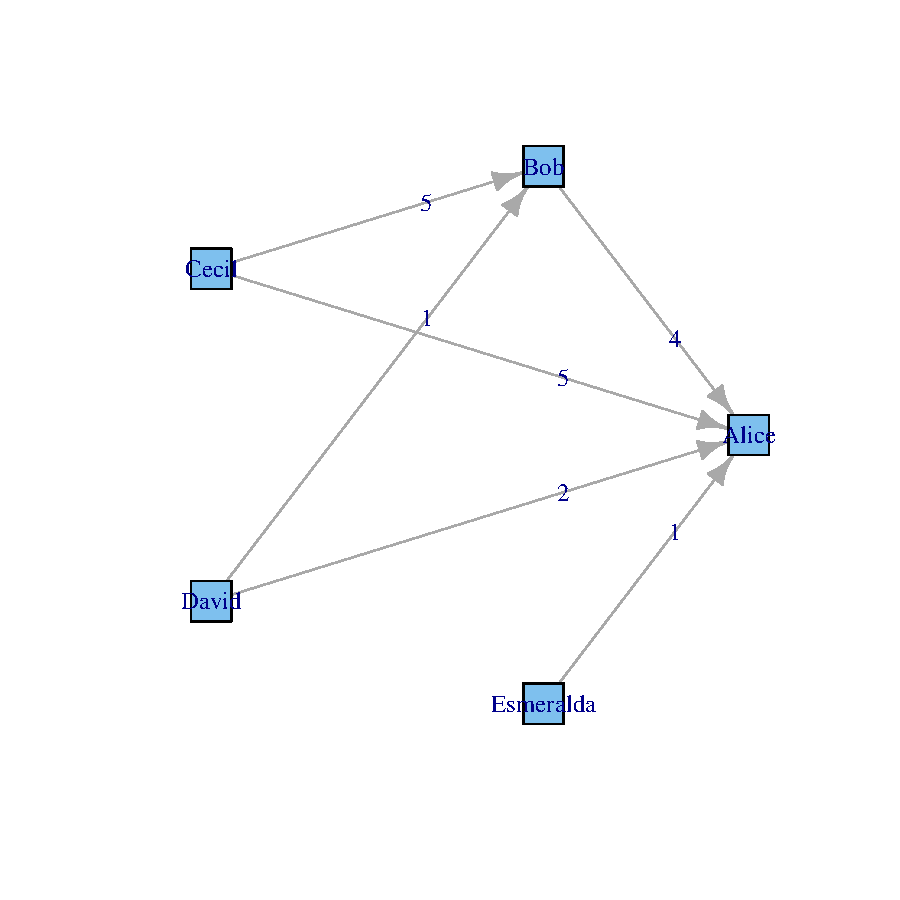
\includegraphics{r3-045}

\section{Transport Problem on Graph}
\label{sec:Transport}


For solution of classic transportation problem, with the use of graph theory, a bipartite graph may be considered, where production points are set in the upper part, while consumption point - in the lower part.  Points of production and consumpton,in pairs, are connected by the edges of the infinite bandwidth and the prices for the unit od the stream Cij.
The upper part artificially is connected  with source vertex. Capacity of the edges from the source vertex to each production point is equal to the store of the commodities in this point. The price for the unit of the flow equals to 0. 
Simillary, the lower part is connected with sink. Capacity of the each of the edge of the consumption point to te sink are equal to necessity of commodity at the point. The price for the unit of production also is equal to one. 
Then, the problem of mincost maxflow should be solved. This solution is analogious with searching for the maxflow in the Ford-Falkerson algorithm. However, despite the use of the shotest complementary flow, the cheapest is used.  Accordingly, ??? (For solution of classic transportation problem, with the use of graph theory, a bipartite graph may be considered, where production points are set in the upper part, while consumption point - in the lower part.  Points of production and consumpton,in pairs, are connected by the edges of the infinite bandwidth and the prices for the unit od the stream Cij.
The upper part artificially is connected  with source vertex. Capacity of the edges from the source vertex to each production point is equal to the store of the commodities in this point. The price for the unit of the flow equals to 0. 
\begin{Schunk}
\begin{Sinput}
> rm(list = ls())
\end{Sinput}
\begin{Soutput}
NULL
\end{Soutput}
\begin{Sinput}
> price_data = c(5, 4, 3, 4, 3, 2, 5, 5, 1, 6, 3, 2)
\end{Sinput}
\begin{Soutput}
 [1] 5 4 3 4 3 2 5 5 1 6 3 2
\end{Soutput}
\begin{Sinput}
> goods_in_stores = data.frame(name = c("s1", "s2", "s3"), flow_in = c(160, 
+     140, 160))
\end{Sinput}
\begin{Soutput}
  name flow_in
1   s1     160
2   s2     140
3   s3     160
\end{Soutput}
\begin{Sinput}
> goods_requr = data.frame(name = c("r1", "r2", "r3", "r4", "r5"), 
+     flow_out = c(80, 80, 60, 80, 80))
\end{Sinput}
\begin{Soutput}
  name flow_out
1   r1       80
2   r2       80
3   r3       60
4   r4       80
5   r5       80
\end{Soutput}
\begin{Sinput}
> ver = data.frame(name = c("S", as.character(goods_in_stores$name), 
+     as.character(goods_requr$name), "D"))
\end{Sinput}
\begin{Soutput}
   name
1     S
2    s1
3    s2
4    s3
5    r1
6    r2
7    r3
8    r4
9    r5
10    D
\end{Soutput}
\begin{Sinput}
> partm_to = NULL
\end{Sinput}
\begin{Soutput}
NULL
\end{Soutput}
\begin{Sinput}
> partm_from = NULL
\end{Sinput}
\begin{Soutput}
NULL
\end{Soutput}
\begin{Sinput}
> flow_m = NULL
\end{Sinput}
\begin{Soutput}
NULL
\end{Soutput}
\begin{Sinput}
> for (v1 in as.character(goods_in_stores$name)) for (v2 in as.character(goods_requr$name)) {
+     if (v1 != v2) {
+         partm_to = c(partm_to, v2)
+         partm_from = c(partm_from, v1)
+         flow_m = c(flow_m, sum(goods_in_stores$flow_in))
+     }
+ }
\end{Sinput}
\begin{Soutput}
NULL
\end{Soutput}
\begin{Sinput}
> partd_to = NULL
\end{Sinput}
\begin{Soutput}
NULL
\end{Soutput}
\begin{Sinput}
> partd_from = NULL
\end{Sinput}
\begin{Soutput}
NULL
\end{Soutput}
\begin{Sinput}
> for (v2 in as.character(goods_requr$name)) {
+     partd_to = c(partd_to, "D")
+     partd_from = c(partd_from, v2)
+ }
\end{Sinput}
\begin{Soutput}
NULL
\end{Soutput}
\begin{Sinput}
> parts_to = NULL
\end{Sinput}
\begin{Soutput}
NULL
\end{Soutput}
\begin{Sinput}
> parts_from = NULL
\end{Sinput}
\begin{Soutput}
NULL
\end{Soutput}
\begin{Sinput}
> for (v2 in as.character(goods_in_stores$name)) {
+     parts_from = c(parts_from, "S")
+     parts_to = c(parts_to, v2)
+ }
\end{Sinput}
\begin{Soutput}
NULL
\end{Soutput}
\begin{Sinput}
> relations <- data.frame(from = c(parts_from, partm_from, partd_from), 
+     to = c(parts_to, partm_to, partd_to), capacity = c(goods_in_stores$flow_in, 
+         flow_m, goods_requr$flow_out))
\end{Sinput}
\begin{Soutput}
   from to capacity
1     S s1      160
2     S s2      140
3     S s3      160
4    s1 r1      460
5    s1 r2      460
6    s1 r3      460
7    s1 r4      460
8    s1 r5      460
9    s2 r1      460
10   s2 r2      460
11   s2 r3      460
12   s2 r4      460
13   s2 r5      460
14   s3 r1      460
15   s3 r2      460
16   s3 r3      460
17   s3 r4      460
18   s3 r5      460
19   r1  D       80
20   r2  D       80
21   r3  D       60
22   r4  D       80
23   r5  D       80
\end{Soutput}
\begin{Sinput}
> g <- graph.data.frame(relations, directed = TRUE, vertices = ver)
\end{Sinput}
\begin{Soutput}
Vertices: 10 
Edges: 23 
Directed: TRUE 
Edges:
                 
[0]  'S'  -> 's1'
[1]  'S'  -> 's2'
[2]  'S'  -> 's3'
[3]  's1' -> 'r1'
[4]  's1' -> 'r2'
[5]  's1' -> 'r3'
[6]  's1' -> 'r4'
[7]  's1' -> 'r5'
[8]  's2' -> 'r1'
[9]  's2' -> 'r2'
[10] 's2' -> 'r3'
[11] 's2' -> 'r4'
[12] 's2' -> 'r5'
[13] 's3' -> 'r1'
[14] 's3' -> 'r2'
[15] 's3' -> 'r3'
[16] 's3' -> 'r4'
[17] 's3' -> 'r5'
[18] 'r1' -> 'D' 
[19] 'r2' -> 'D' 
[20] 'r3' -> 'D' 
[21] 'r4' -> 'D' 
[22] 'r5' -> 'D' 
\end{Soutput}
\begin{Sinput}
> print(g, e = TRUE, v = TRUE)
\end{Sinput}
\begin{Soutput}
Vertices: 10 
Edges: 23 
Directed: TRUE 
Vertex attributes:
    name
[0]    S
[1]   s1
[2]   s2
[3]   s3
[4]   r1
[5]   r2
[6]   r3
[7]   r4
[8]   r5
[9]    D
Edges and their attributes:
                  capacity
[0]  'S'  -> 's1'      160
[1]  'S'  -> 's2'      140
[2]  'S'  -> 's3'      160
[3]  's1' -> 'r1'      460
[4]  's1' -> 'r2'      460
[5]  's1' -> 'r3'      460
[6]  's1' -> 'r4'      460
[7]  's1' -> 'r5'      460
[8]  's2' -> 'r1'      460
[9]  's2' -> 'r2'      460
[10] 's2' -> 'r3'      460
[11] 's2' -> 'r4'      460
[12] 's2' -> 'r5'      460
[13] 's3' -> 'r1'      460
[14] 's3' -> 'r2'      460
[15] 's3' -> 'r3'      460
[16] 's3' -> 'r4'      460
[17] 's3' -> 'r5'      460
[18] 'r1' -> 'D'        80
[19] 'r2' -> 'D'        80
[20] 'r3' -> 'D'        60
[21] 'r4' -> 'D'        80
[22] 'r5' -> 'D'        80
Vertices: 10 
Edges: 23 
Directed: TRUE 
Edges:
                 
[0]  'S'  -> 's1'
[1]  'S'  -> 's2'
[2]  'S'  -> 's3'
[3]  's1' -> 'r1'
[4]  's1' -> 'r2'
[5]  's1' -> 'r3'
[6]  's1' -> 'r4'
[7]  's1' -> 'r5'
[8]  's2' -> 'r1'
[9]  's2' -> 'r2'
[10] 's2' -> 'r3'
[11] 's2' -> 'r4'
[12] 's2' -> 'r5'
[13] 's3' -> 'r1'
[14] 's3' -> 'r2'
[15] 's3' -> 'r3'
[16] 's3' -> 'r4'
[17] 's3' -> 'r5'
[18] 'r1' -> 'D' 
[19] 'r2' -> 'D' 
[20] 'r3' -> 'D' 
[21] 'r4' -> 'D' 
[22] 'r5' -> 'D' 
\end{Soutput}
\begin{Sinput}
> plot(g, vertex.shape = "crectangle", vertex.label = ver$name, 
+     edge.label = relations$capacity, layout = layout.kamada.kawai(g))
\end{Sinput}
\begin{Soutput}
NULL
\end{Soutput}
\begin{Sinput}
> s = graph.maxflow(g, "S", "D", capacity = relations$capacity)
\end{Sinput}
\begin{Soutput}
[1] 380
\end{Soutput}
\begin{Sinput}
> cat("maxflow =", s, "\n")
\end{Sinput}
\begin{Soutput}
maxflow = 380 
NULL
\end{Soutput}
\end{Schunk}
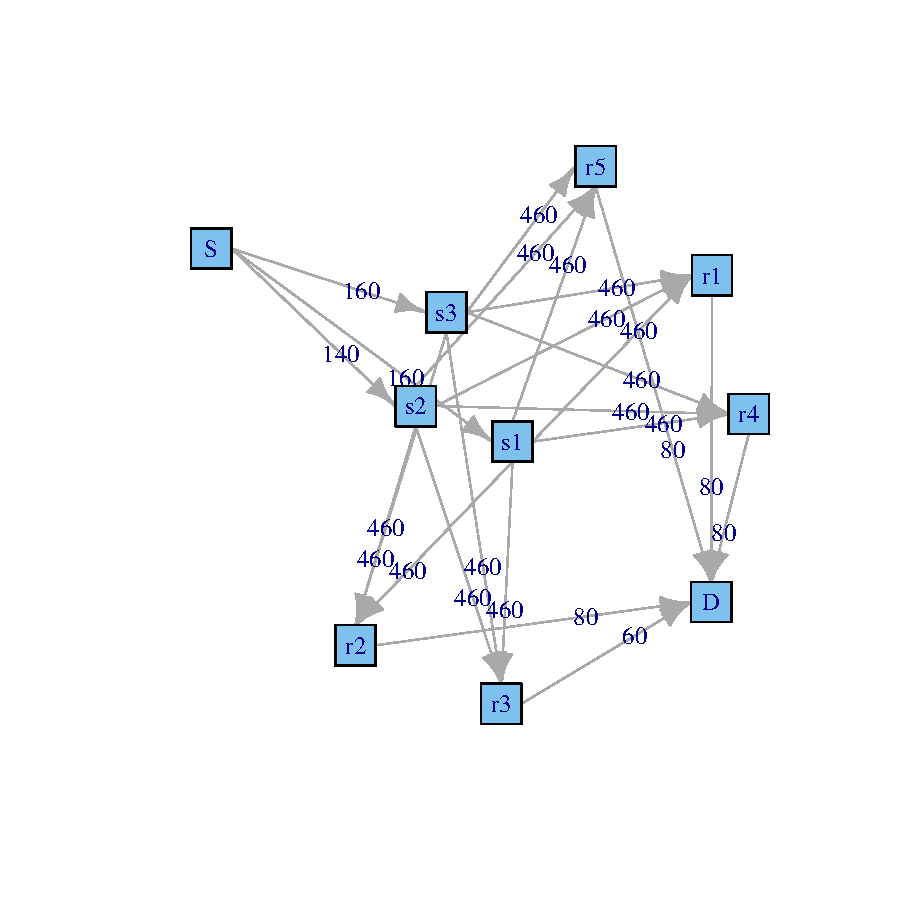
\includegraphics{r3-046}


\section{Text mining}
\label{sec:textmining}

\begin{Schunk}
\begin{Sinput}
> library("tm")
\end{Sinput}
\begin{Soutput}
 [1] "tm"        "igraph"    "lpSolve"   "stats"     "graphics"  "grDevices"
 [7] "utils"     "datasets"  "methods"   "base"     
\end{Soutput}
\begin{Sinput}
> docs1 <- data.frame(docs = c("Для большинства экземпляров вид бабоч также характерна своеобразная червеобразная личинка с недоразвитыми брюшными ногами, называемая гусеницей. ", 
+     "ископаемые останки этого вид которых известны начиная с юрского периода, ", 
+     "в настоящее время вид  бабоч — один из наиболее богатых вид отряд насекомых, ", 
+     "представители вид которого распространены на всех континентах, за исключением Антарктиды."))
\end{Sinput}
\begin{Soutput}
                                                                                                                                               docs
1 Для большинства экземпляров вид бабоч также характерна своеобразная червеобразная личинка с недоразвитыми брюшными ногами, называемая гусеницей. 
2                                                                         ископаемые останки этого вид которых известны начиная с юрского периода, 
3                                                                     в настоящее время вид  бабоч — один из наиболее богатых вид отряд насекомых, 
4                                                         представители вид которого распространены на всех континентах, за исключением Антарктиды.
\end{Soutput}
\begin{Sinput}
> docs2 <- data.frame(docs = c("Теорем о бабоч является классической теорем планиметрии.", 
+     "теорем Опубликована в 1815 году в англ мужском журнале «Gentleman's Diary» (англ.). ", 
+     " авторство теорем приписывают англ математику Уильяму Джорджу Горнеру. ", 
+     "Сформулировать теорем можно следующим образом:"))
\end{Sinput}
\begin{Soutput}
                                                                                  docs
1                             Теорем о бабоч является классической теорем планиметрии.
2 теорем Опубликована в 1815 году в англ мужском журнале «Gentleman's Diary» (англ.). 
3               авторство теорем приписывают англ математику Уильяму Джорджу Горнеру. 
4                                       Сформулировать теорем можно следующим образом:
\end{Soutput}
\begin{Sinput}
> ds1 <- DataframeSource(docs1)
\end{Sinput}
\begin{Soutput}
$DefaultReader
function (...) 
{
    function(elem, language, id) PlainTextDocument(elem$content, 
        id = id, language = language)
}
<environment: namespace:tm>
attr(,"class")
[1] "FunctionGenerator" "function"         

$Encoding
[1] "UTF-8"

$Length
[1] 4

$LoDSupport
[1] FALSE

$Names
[1] "1" "2" "3" "4"

$Position
[1] 0

$Vectorized
[1] TRUE

$Content
                                                                                                                                               docs
1 Для большинства экземпляров вид бабоч также характерна своеобразная червеобразная личинка с недоразвитыми брюшными ногами, называемая гусеницей. 
2                                                                         ископаемые останки этого вид которых известны начиная с юрского периода, 
3                                                                     в настоящее время вид  бабоч — один из наиболее богатых вид отряд насекомых, 
4                                                         представители вид которого распространены на всех континентах, за исключением Антарктиды.

attr(,"class")
[1] "DataframeSource" "Source"         
\end{Soutput}
\begin{Sinput}
> ds2 <- DataframeSource(docs2)
\end{Sinput}
\begin{Soutput}
$DefaultReader
function (...) 
{
    function(elem, language, id) PlainTextDocument(elem$content, 
        id = id, language = language)
}
<environment: namespace:tm>
attr(,"class")
[1] "FunctionGenerator" "function"         

$Encoding
[1] "UTF-8"

$Length
[1] 4

$LoDSupport
[1] FALSE

$Names
[1] "1" "2" "3" "4"

$Position
[1] 0

$Vectorized
[1] TRUE

$Content
                                                                                  docs
1                             Теорем о бабоч является классической теорем планиметрии.
2 теорем Опубликована в 1815 году в англ мужском журнале «Gentleman's Diary» (англ.). 
3               авторство теорем приписывают англ математику Уильяму Джорджу Горнеру. 
4                                       Сформулировать теорем можно следующим образом:

attr(,"class")
[1] "DataframeSource" "Source"         
\end{Soutput}
\begin{Sinput}
> r1 = Corpus(ds1)
\end{Sinput}
\begin{Soutput}
A corpus with 4 text documents
\end{Soutput}
\begin{Sinput}
> r2 = Corpus(ds2)
\end{Sinput}
\begin{Soutput}
A corpus with 4 text documents
\end{Soutput}
\begin{Sinput}
> r = c(r1, r2)
\end{Sinput}
\begin{Soutput}
A corpus with 8 text documents
\end{Soutput}
\begin{Sinput}
> sw1 = c("kterou", "tomu", "které", "tohoto", "tzv")
\end{Sinput}
\begin{Soutput}
[1] "kterou" "tomu"   "které"  "tohoto" "tzv"   
\end{Soutput}
\begin{Sinput}
> sw1 = c("следующим", "можно", "образом", 
+     "tzv")
\end{Sinput}
\begin{Soutput}
[1] "следующим" "можно"     "образом"   "tzv"      
\end{Soutput}
\begin{Sinput}
> sw2 = c("этого", "также", "которых", "которого", 
+     "для", "всех")
\end{Sinput}
\begin{Soutput}
[1] "этого"    "также"    "которых"  "которого" "для"      "всех"    
\end{Soutput}
\begin{Sinput}
> sw = c(sw1, sw2)
\end{Sinput}
\begin{Soutput}
 [1] "следующим" "можно"     "образом"   "tzv"       "этого"     "также"    
 [7] "которых"   "которого"  "для"       "всех"     
\end{Soutput}
\begin{Sinput}
> tdm1 = TermDocumentMatrix(r1, control = list(removePunctuation = TRUE, 
+     stopwords = sw, minWordLength = 3))
\end{Sinput}
\begin{Soutput}
A term-document matrix (31 terms, 4 documents)

Non-/sparse entries: 35/89
Sparsity           : 72%
Maximal term length: 14 
Weighting          : term frequency (tf)
\end{Soutput}
\begin{Sinput}
> tdm2 = TermDocumentMatrix(r2, control = list(removePunctuation = TRUE, 
+     stopwords = sw, minWordLength = 3))
\end{Sinput}
\begin{Soutput}
A term-document matrix (20 terms, 4 documents)

Non-/sparse entries: 24/56
Sparsity           : 70%
Maximal term length: 14 
Weighting          : term frequency (tf)
\end{Soutput}
\begin{Sinput}
> tdm3 = TermDocumentMatrix(r, control = list(removePunctuation = TRUE, 
+     stopwords = sw, minWordLength = 3))
\end{Sinput}
\begin{Soutput}
A term-document matrix (50 terms, 8 documents)

Non-/sparse entries: 59/341
Sparsity           : 85%
Maximal term length: 14 
Weighting          : term frequency (tf)
\end{Soutput}
\begin{Sinput}
> dtm3 = TermDocumentMatrix(r, control = list(removePunctuation = TRUE, 
+     stopwords = sw, minWordLength = 3))
\end{Sinput}
\begin{Soutput}
A term-document matrix (50 terms, 8 documents)

Non-/sparse entries: 59/341
Sparsity           : 85%
Maximal term length: 14 
Weighting          : term frequency (tf)
\end{Soutput}
\begin{Sinput}
> t11 = NULL
\end{Sinput}
\begin{Soutput}
NULL
\end{Soutput}
\begin{Sinput}
> i = 0
\end{Sinput}
\begin{Soutput}
[1] 0
\end{Soutput}
\begin{Sinput}
> keyterms = findFreqTerms(tdm3, 2, 5)
\end{Sinput}
\begin{Soutput}
[1] "англ"   "бабоч"  "вид"    "теорем"
\end{Soutput}
\begin{Sinput}
> for (term in keyterms) {
+     i = i + 1
+     t11 = c(t11, data.frame(findAssocs(tdm3, keyterms[i], 0.2), 
+         row.names = NULL))
+ }
\end{Sinput}
\begin{Soutput}
NULL
\end{Soutput}
\begin{Sinput}
> print(t11)
\end{Sinput}
\begin{Soutput}
$findAssocs.tdm3..keyterms.i...0.2.
 [1] 1.00 0.88 0.88 0.88 0.88 0.88 0.88 0.88 0.34 0.34 0.34 0.34 0.34 0.34 0.29

$findAssocs.tdm3..keyterms.i...0.2.
 [1] 1.00 0.49 0.49 0.49 0.49 0.49 0.49 0.49 0.49 0.49 0.49 0.49 0.49 0.49 0.49
[16] 0.49 0.49 0.49 0.49 0.49 0.49 0.49 0.42

$findAssocs.tdm3..keyterms.i...0.2.
 [1] 1.00 0.75 0.75 0.75 0.75 0.75 0.75 0.75 0.42 0.20 0.20 0.20 0.20 0.20 0.20
[16] 0.20 0.20 0.20 0.20 0.20 0.20 0.20 0.20 0.20 0.20 0.20 0.20 0.20 0.20 0.20
[31] 0.20

$findAssocs.tdm3..keyterms.i...0.2.
 [1] 1.00 0.75 0.75 0.75 0.29 0.20 0.20 0.20 0.20 0.20 0.20 0.20 0.20 0.20 0.20
[16] 0.20 0.20 0.20 0.20

$findAssocs.tdm3..keyterms.i...0.2.
 [1] 1.00 0.88 0.88 0.88 0.88 0.88 0.88 0.88 0.34 0.34 0.34 0.34 0.34 0.34 0.29

$findAssocs.tdm3..keyterms.i...0.2.
 [1] 1.00 0.49 0.49 0.49 0.49 0.49 0.49 0.49 0.49 0.49 0.49 0.49 0.49 0.49 0.49
[16] 0.49 0.49 0.49 0.49 0.49 0.49 0.49 0.42

$findAssocs.tdm3..keyterms.i...0.2.
 [1] 1.00 0.75 0.75 0.75 0.75 0.75 0.75 0.75 0.42 0.20 0.20 0.20 0.20 0.20 0.20
[16] 0.20 0.20 0.20 0.20 0.20 0.20 0.20 0.20 0.20 0.20 0.20 0.20 0.20 0.20 0.20
[31] 0.20

$findAssocs.tdm3..keyterms.i...0.2.
 [1] 1.00 0.75 0.75 0.75 0.29 0.20 0.20 0.20 0.20 0.20 0.20 0.20 0.20 0.20 0.20
[16] 0.20 0.20 0.20 0.20
\end{Soutput}
\end{Schunk}
\includegraphics{r3-047}


\end{document}
